% !TEX root = main.tex
% !TeX program = xelatex
\documentclass[UTF8,a4paper,12pt,fontset=fandol]{ctexart}
\usepackage[left=2.5cm,right=2.5cm,top=2.4cm,bottom=2.4cm]{geometry}
\usepackage{amsmath,amssymb,bm}
\usepackage{booktabs,longtable,tabularx,array,multirow}
\usepackage{graphicx,float,subcaption}
\usepackage{xcolor}
\usepackage{enumitem}
\usepackage{setspace}
\usepackage{fancyhdr}
\usepackage{hyperref}
\usepackage{bookmark}
\usepackage{listings}
\usepackage{caption}
\usepackage{chngcntr}

\hypersetup{colorlinks=true,linkcolor=black,citecolor=black,urlcolor=blue}
% 论文图像统一放在 paper/figures 中，使本目录可独立编译与提交。
\graphicspath{{figures/}}
\captionsetup{font=small,labelsep=quad}
\captionsetup[table]{position=top}
\renewcommand{\figurename}{图}
\captionsetup[figure]{
    name=图,
    labelsep=space,
    labelfont=bf,
    textfont=bf
}
\captionsetup[figure]{labelfont=bf,textfont=bf}
% 适度收紧正文行距，保持可读性并减少分页碎片
\setstretch{1.12}
\raggedbottom
\setlength{\parindent}{2em}
\setlength{\parskip}{0pt}
\setlist{nosep,leftmargin=2em}
\pagestyle{fancy}
\fancyhf{}
\cfoot{\thepage}
\renewcommand{\headrulewidth}{0pt}
\renewcommand{\arraystretch}{1.05}
\setlength{\textfloatsep}{6pt plus 2pt minus 2pt}
\setlength{\intextsep}{6pt plus 2pt minus 2pt}
\setlength{\floatsep}{5pt plus 2pt minus 2pt}
\ctexset{section={beforeskip=1.2ex plus .2ex minus .1ex, afterskip=.7ex plus .1ex minus .1ex},
  subsection={beforeskip=.9ex plus .1ex minus .1ex, afterskip=.4ex plus .1ex minus .1ex}}
\newcolumntype{Y}{>{\centering\arraybackslash}X}
\newcolumntype{L}{>{\raggedright\arraybackslash}X}
\newcommand{\dif}{\mathop{}\!\mathrm{d}}
\newcommand{\VaR}{\operatorname{VaR}}
\newcommand{\CVaR}{\operatorname{CVaR}}
\newcommand{\logit}{\operatorname{logit}}
\numberwithin{equation}{section}
\counterwithin{table}{section}
\renewcommand{\thefigure}{\arabic{figure}}
\renewcommand{\thetable}{\thesection-\arabic{table}}

\lstset{
  language=Python,
  basicstyle=\ttfamily\scriptsize,
  keywordstyle=\color{blue!70!black},
  commentstyle=\color{green!45!black},
  stringstyle=\color{orange!70!black},
  numbers=left,
  numberstyle=\tiny\color{gray},
  frame=single,
  breaklines=true,
  showstringspaces=false,
  tabsize=4,
  columns=fullflexible
}

\title{\heiti\bfseries 微网与外部电网电力调控策略优化的研究}
\author{}
\date{}

\begin{document}
\vspace{-5.5em}
\maketitle
\vspace{-2.2em}

\begin{abstract}
\normalsize
针对光伏出力、居民负荷及电价变化共同作用下微网购电与储能调度问题，本文基于负荷预测、光伏预测和分时电价数据，在满足供需平衡、储能容量及充放电功率等运行约束的条件下，以微网运行总成本最小为目标，分别研究日前计划、日内调整及波动电价下的优化调度策略。

\textbf{针对问题一，}将一天划分为144个十分钟时段，以购电量、充放电量、弃光量和储能电量为决策变量，建立\textbf{光伏—储能联合优化调度模型}，并采用\textbf{混合整数线性规划}进行求解。在允许弃光且不向外部电网售电的条件下，模型得到的最优购电费用约为\textbf{35126.95元}，较无储能方案降低\textbf{26.90\%}，且各时段用电需求均得到满足，储能运行状态始终处于安全范围内。

\textbf{针对问题二，}考虑预测误差对日前计划和紧急购电的影响，采用\textbf{严格因果的动态净负荷分位数预测方法}，并结合日前\textbf{混合整数规划模型}制定购电与储能计划。在固定电价条件下，通过在0.50--0.95分位数候选集中依据历史运行成本进行滚动选择，得到全年总成本为\textbf{16413518.08元}，紧急购电量为\textbf{622766.43千瓦时}。

\textbf{针对问题三，}采用\textbf{滚动时域优化方法}，利用0时、6时、12时和18时发布的最新预测信息，动态更新尚未执行的调度计划。在固定电价条件下，全年总成本为\textbf{16130891.40元}，较问题二降低\textbf{1.72\%}。进一步增加3时、9时、15时和21时的预测更新后，计算得到毛信息价值为\textbf{-71161.01元}，表明在当前运行机制下增加预测更新时间点并不能带来经济收益。

\textbf{针对问题四，}将附件4中的波动电价引入\textbf{日前计划与滚动调整双策略模型}，分别制定日前调度方案和实时滚动修正方案。结果表明，日前策略总成本为17148794.62元，滚动调整策略总成本为\textbf{16864403.38元}，较日前策略降低\textbf{1.66\%}；两种策略均满足供需平衡及储能运行约束，说明滚动调整策略能够更有效地利用最新预测信息和动态电价降低微网运行成本。

\par\medskip
\noindent\textbf{关键词：}光伏—储能联合优化调度；混合整数线性规划；动态净负荷分位数预测；滚动时域优化；波动电价\par
\end{abstract}
\clearpage



\section{问题重述}

\subsection{问题的背景}

随着光伏等分布式电源广泛接入居民用电系统，能够在一定区域内组织发电与用电的微网逐渐得到应用，既有助于新能源就地利用，也可减轻集中并网带来的压力。对于仍与外网相连的微网，运行时需结合小区负载、光伏发电量和电池余量安排购电量及充放电量，在保障基本供电要求的同时控制成本。一方面，光伏发电量具有明显的日内变化，其发电高峰未必与居民用电高峰重合，局部时段可能出现光伏电能富余，而其他时段仍需依赖从外部电网购电。另一方面，微网储能虽然能够协调转移电能的使用时刻，却受到容量、充放电功率和能量转换损耗的限制。因此，仅依据“低价充电、高价放电”的经验规则，难以协调光伏消纳、购电支出和后续时段的供电需求。

当调度由基于确定性数据的单日计划扩展至多日连续运行时，问题进一步表现为预测与决策之间的相互影响。计划购电偏少会增加高价紧急购电的需求；计划购电偏多则可能导致部分已购电量无法充分利用、但仍需支付费用。即使日内能够更新光伏预报，调整计划也伴随着额外交易费用，因此，预测更新能否带来实际费用降低，需要通过计算完整的调度成本衡量。

近年来的相关研究为上述问题提供了方法依据。2022年发表于《可再生能源》的研究将实际负荷、可再生能源数据及预测误差纳入经济模型预测控制框架，强调利用滚动决策适应实际运行状态[1]。2023年的风险感知微网能源管理研究指出，应系统考虑发电与用电预测的不确定性，同时控制随机优化的计算负担[2]。据此，本题需要围绕“物理约束下的经济调度---预测误差下的补救决策---信息更新下的动态调整”建立统一研究框架。

\begin{figure}[htbp]
    \centering
    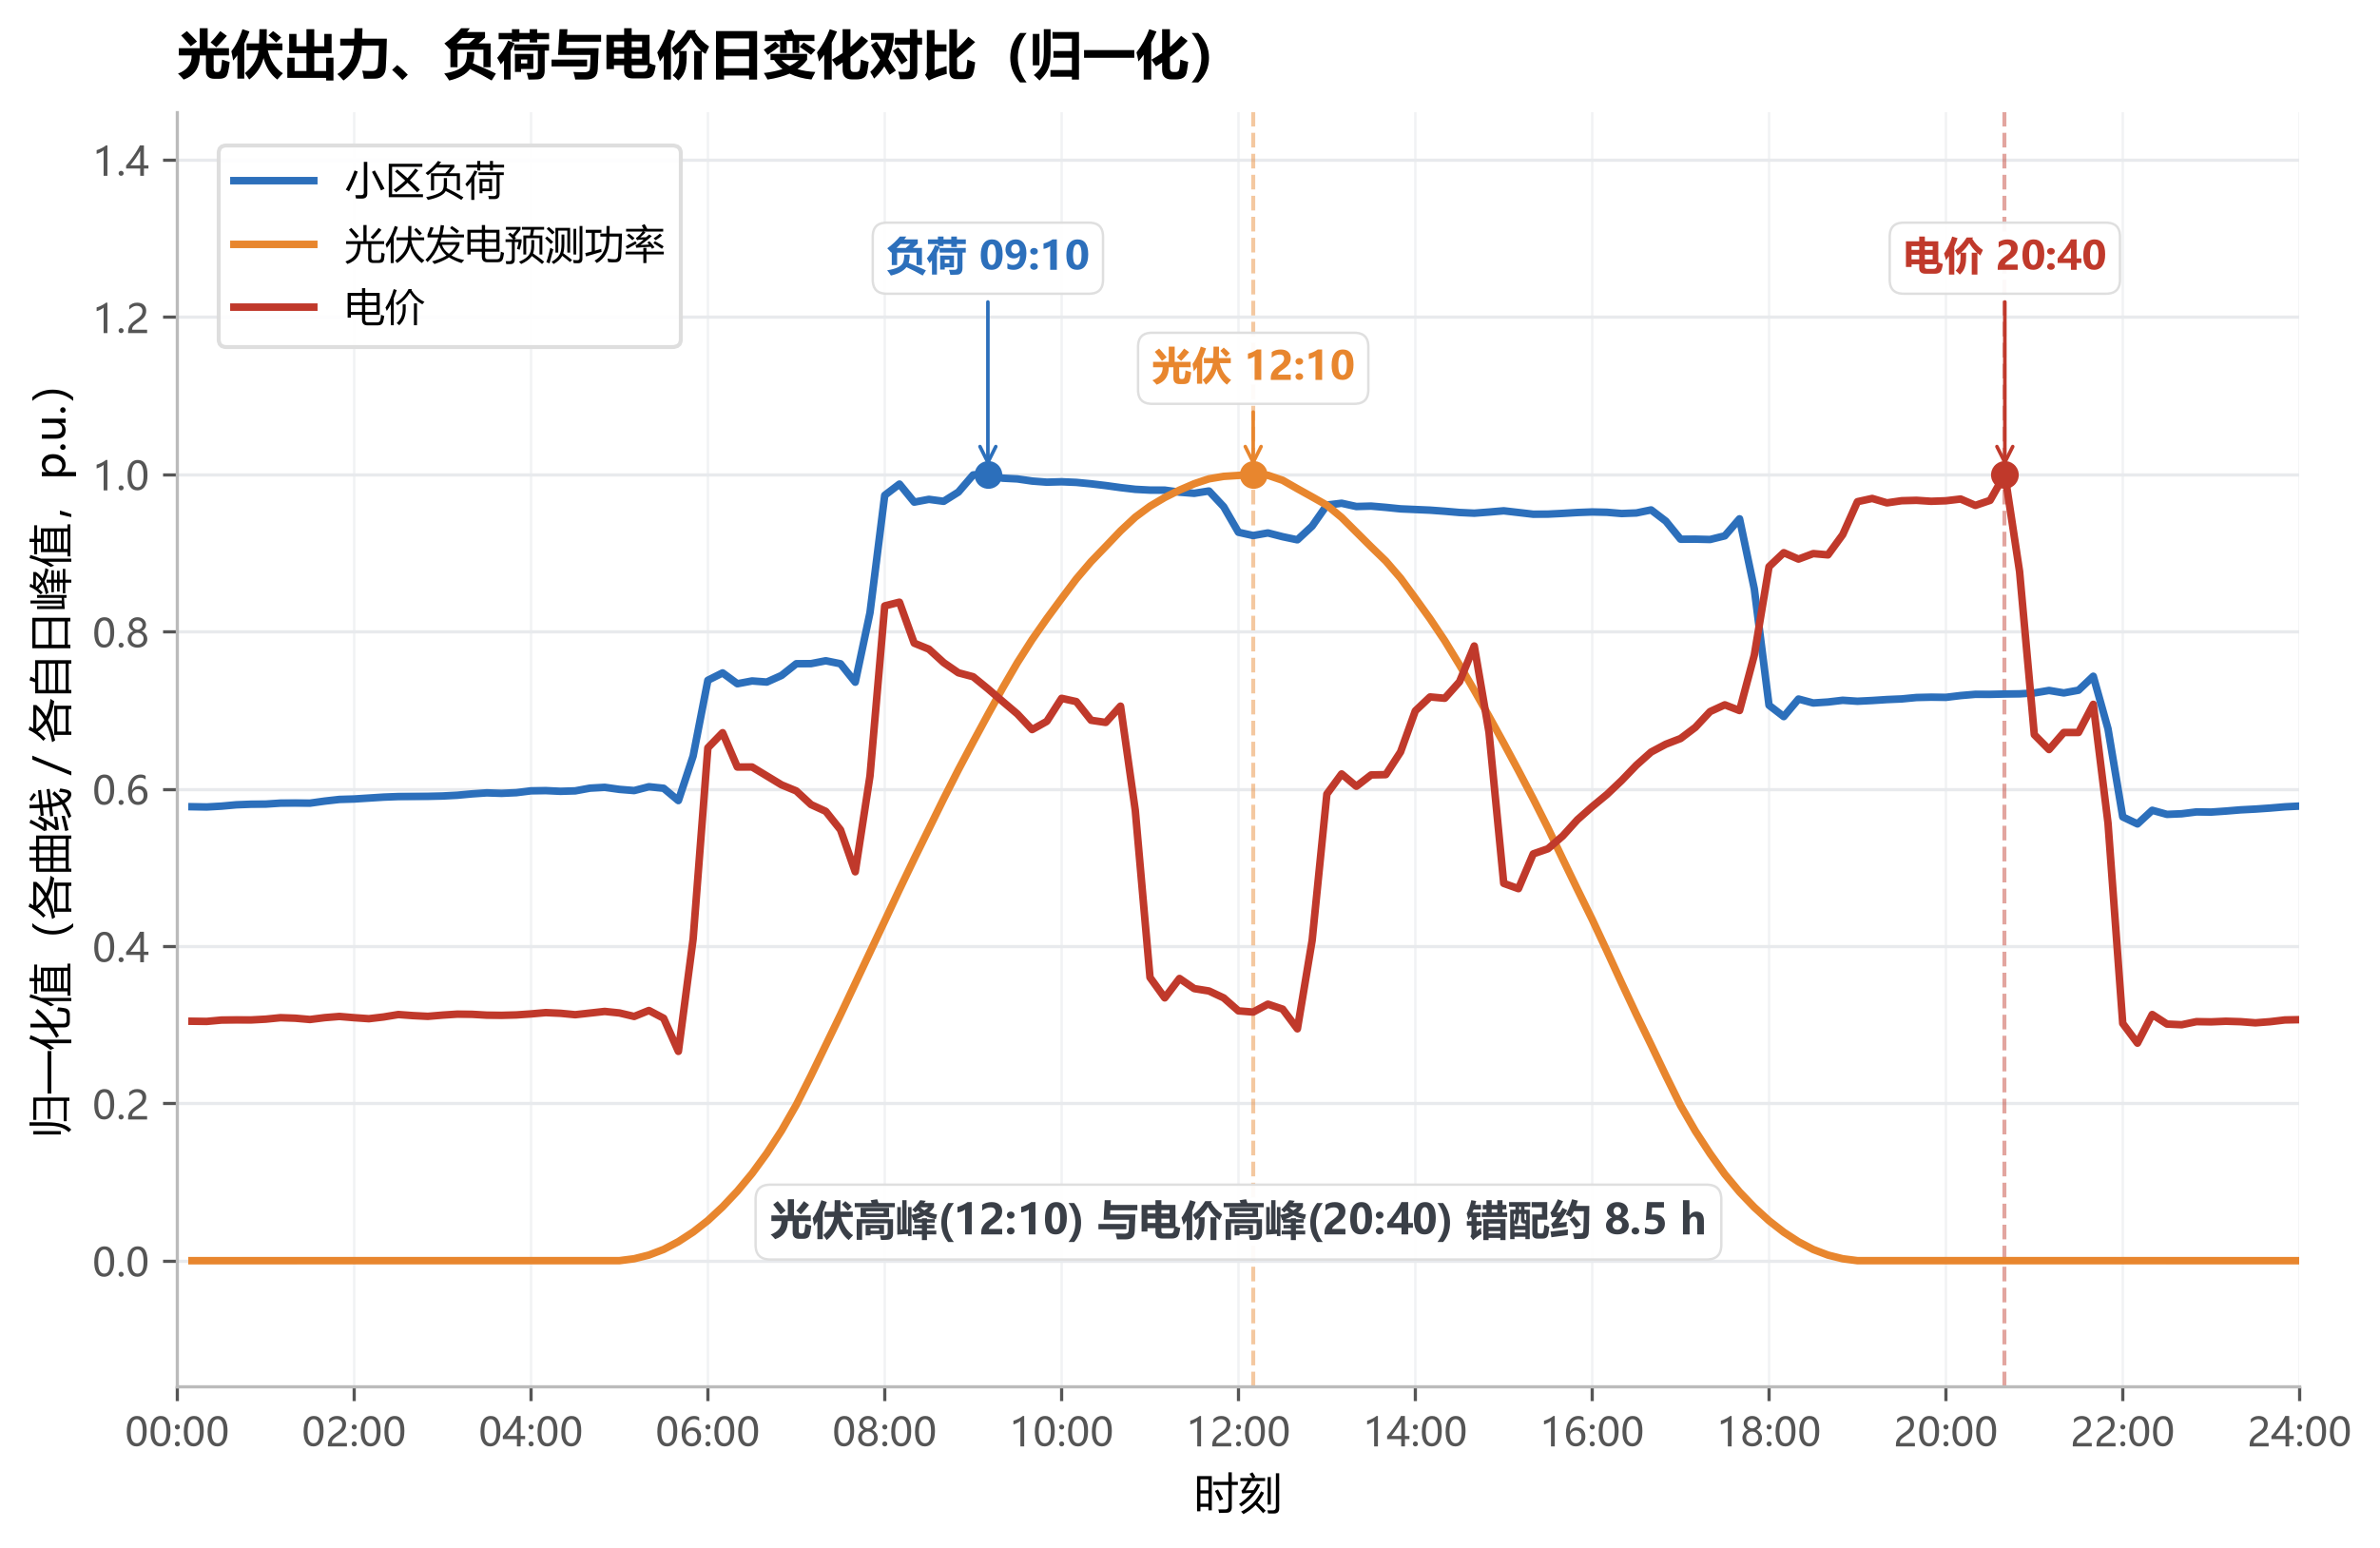
\includegraphics[width=0.9\textwidth]{图1_光伏出力、负荷与电价日变化对比.png}
    \caption{光伏出力、负荷与电价日变化对比}
    \label{fig:pv-load-daily}
\end{figure}

\subsection{问题的重新表述}



\textbf{问题1：}（1）依据附件1给出的固定电价、小区负载和光伏预测数据，建立购电量与储能充放电量的联合优化模型；（2）在微网供量不低于负载、储能容量和功率受限的条件下，使全天购电费用最小；（3）给出指定时段及全天的购电量和购电费、充放电量、0点和24点储电量，并将完整策略写入结果文件。\par

\textbf{问题2：}（1）依据附件1的固定电价和附件2的全年实际负荷、光伏数据，仅利用决策日前可获得的历史信息预测次日供需；（2）在每天0:00制定全天计划，以五倍电价的紧急购电弥补实际执行中的供电缺口；（3）给出指定日期的购电量和购电费、充放电量与紧急购电结果，并形成2025年2月1日至12月31日的完整策略。\par

\textbf{问题3：}（1）依据附件3在每天四个时间节点发布的光伏发电功率预报，对尚未执行购电的时段滚动更新调整购电量；（2）综合计划购电费、上调费用、下调违约费用和紧急购电费，建立固定已执行决策的滚动调整模型；（3）给出指定日期及全年策略，并通过新增预报时点的成本变化判断是否有必要增加预报节点。\par

\textbf{问题4：}（1）将附件4的波动电价分别代入问题2的日前计划机制和问题3的滚动调整机制；（2）在相同供需条件下重新求解两类策略；（3）比较固定电价与波动电价下的成本、紧急购电及稳定性，并说明电价信息可得范围对结论的影响。\par

\subsection{我们的工作}

\begin{figure}[H]
    \centering
    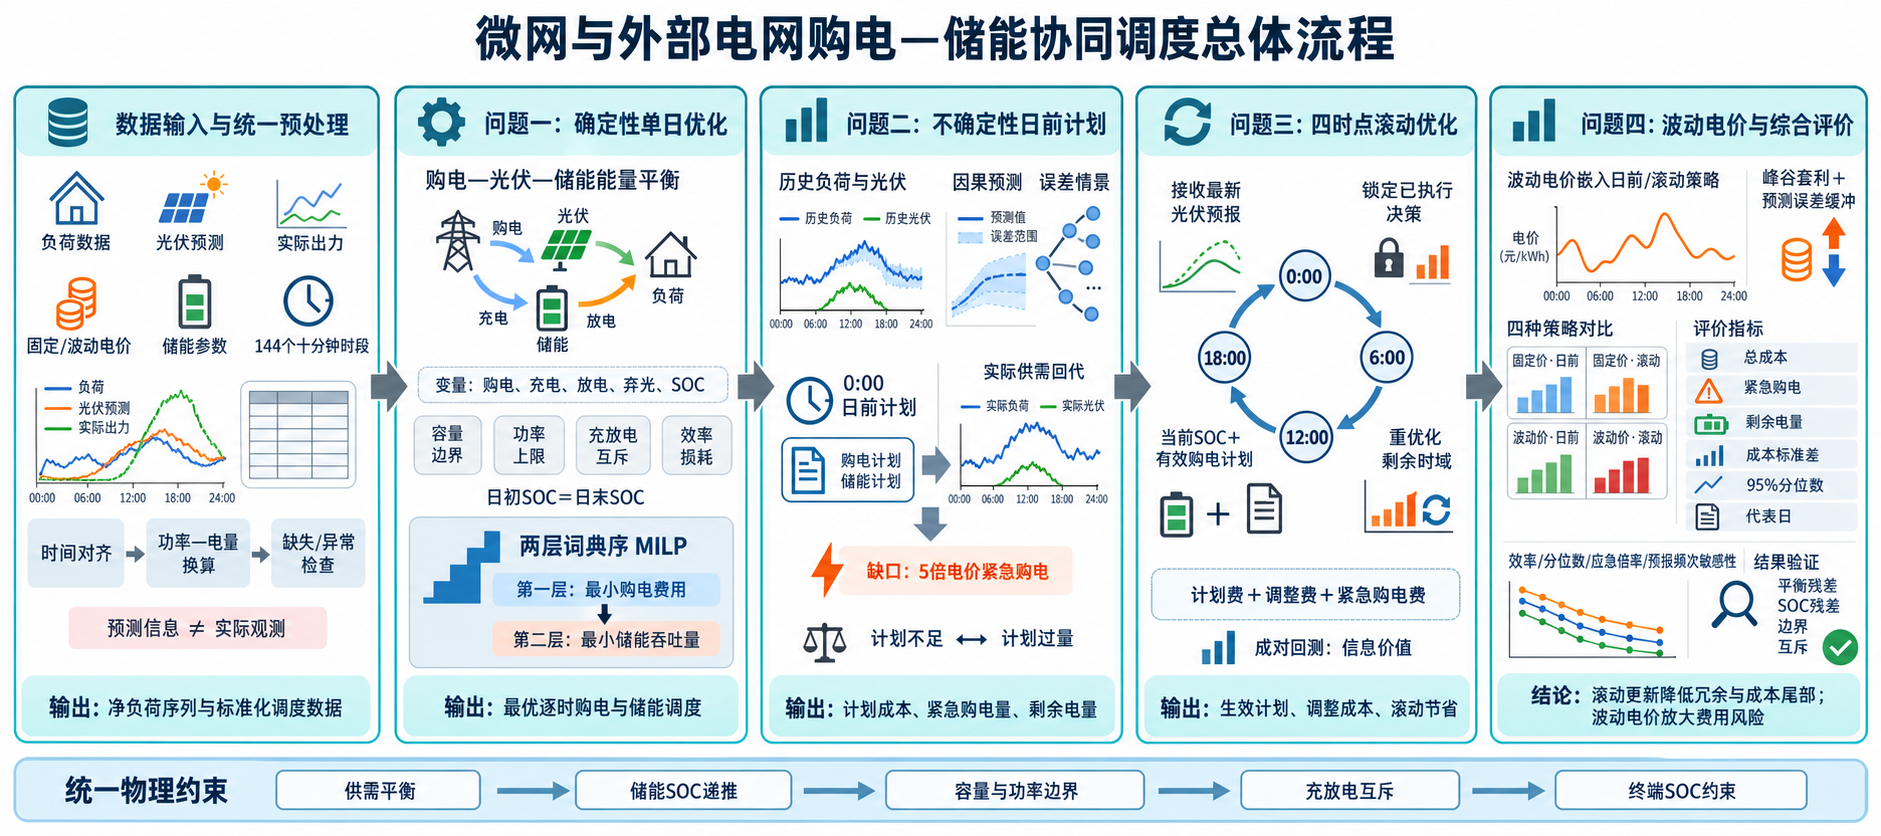
\includegraphics[width=\textwidth]{图2_微网与外部电网购电储能协同调度总体流程.png}
    \caption{微网与外部电网购电—储能协同调度总体流程}
    \label{fig:overall-workflow}
\end{figure}

\section{问题分析}

\subsection{总体思路}

本题整体采用“数据处理与因果预测---约束优化---滚动执行---对照检验”的思路。以供需平衡和储能状态递推构成统一物理模型，逐步增加紧急购电、计划调整和电价不确定性。购电、调整与补救费用共同构成总成本，属于具有多个成本分项的单目标优化；问题一再以两层词典序方式处理等价方案选择。

\subsection{问题一分析}

关键矛盾是：降低当前购电费用与保留后续可用储能之间的跨时段权衡。首先统一功率、电量与时间索引，计算并识别出净负荷及光伏富余区间；其次建立购电、充放电和储能状态变量，以二元变量保证充放电状态互斥，并施加容量、功率及单日内首末储能相等的约束；最后先最小化购电费，再在购电费不变的情况下最小化充放电次数，通过约束回代和线性松弛下界检验方案。

\subsection{问题二分析}

关键矛盾是：当计划购电量不足引发高价补购，而过度采购仍需承担冗余计划费用。先按时间顺序利用历史数据预测未来单日负荷和光伏，再根据预测残差构造保留时间相关性的情景；随后建立日前计划与实时补救相衔接的两阶段模型。执行时仅依据当时可用信息调整储能和紧急购电，保持跨日状态连续，避免利用未来实际值获得不可实现的策略优势。

\subsection{问题三分析}

关键矛盾是：新预报可能降低供需偏差，但修改计划需要支付费用。先将整点预报统一至十分钟网格，再于各发布时间更新剩余时域的预测，固定已执行决策，以当前储能和有效购电计划为起点进行滚动优化。结算时区分原始计划、增减调整量和紧急购电。新增预报时点通过成对回测比较净成本变化，其收益须覆盖信息获取及调整成本。

\section{模型假设}
\begin{enumerate}
\item \textbf{各时段数据以平均水平代表，调度决策不使用未来信息。}
将运行过程按十分钟划分。每个时段内，负荷、光伏发电量及电价均视为稳定不变。对于问题二至问题四，仅使用决策时间点之前已观测或已发布的信息，并按照统一方法将整点预报信息延用至后十分钟区间，以保证预测与滚动优化方案具有可执行性。

\item \textbf{微网储能效率与可用容量在研究期间保持稳定。}
将题目中的90\%分别作为充电效率和放电效率，不考虑自放电，以及温度、充放电功率和循环老化对储能性能的影响。在此基础上，采用线性的储能状态递推模型描述电量变化。

\item \textbf{微网按单节点处理，允许弃电但不考虑对外售电。}
忽略微网内部线路损耗、电压约束，同时假设外部电网能够正常供电。光伏发电出现富余时可直接弃用；已购电量若未被负荷或储能消纳，则不予退款，也不产生售电收益，从而保证各时段的电量平衡。

\item \textbf{滚动调整仅作用于尚未执行的时段。}
每次更新预报时，已执行时段的购电、充放电及储能状态均保持不变；仅对当前时刻之后的剩余时段重新优化，且调整费用按最终生效计划相对原始计划费用的净变化计入。

\item \textbf{储能状态在相邻日期之间连续。}
在问题一中，按照题意要求当日0点与24点储电量相等。对于问题二至问题四，次日初始储能状态取前一日的实际末状态，同时不再要求当日0点和24点的储电量一致。
\end{enumerate}

\section{符号说明}

为避免功率、电量和信息时点混用，本文统一以每个十分钟时段的交流侧电量建立供需平衡，以电池内部电量描述SOC。表\ref{tab:symbols}仅列出后文实际使用的符号；上标“act”“for”分别表示实际值和预测值，上标“0”表示日前原计划。

\begingroup
\small
\setlength{\tabcolsep}{4pt}
\begin{longtable}{>{\centering\arraybackslash}p{0.20\textwidth}>{\raggedright\arraybackslash}p{0.59\textwidth}>{\centering\arraybackslash}p{0.14\textwidth}}
\caption{主要符号及其含义}\label{tab:symbols}\\
\toprule
符号 & 含义 & 单位\\
\midrule
\endfirsthead
\multicolumn{3}{c}{表\thetable\quad 主要符号及其含义（续）}\\
\toprule
符号 & 含义 & 单位\\
\midrule
\endhead
\midrule
\multicolumn{3}{r}{续下页}\\
\endfoot
\bottomrule
\endlastfoot
\multicolumn{3}{l}{\textbf{索引与时间参数}}\\
$d$ & 日期索引，按自然日递增 & 天\\
$t$ & 日内十分钟时段索引，$t=1,\ldots,144$ & --\\
$r$ & 日内预测发布时间索引，问题三取0、6、12、18时 & 时\\
$\Delta t$ & 时段长度，$\Delta t=1/6$ & h\\
\midrule
\multicolumn{3}{l}{\textbf{实际量、预测量与价格参数}}\\
$L^{P,\mathrm{act}}_{d,t}$ & 实际负荷功率 & kW\\
$P^{P,\mathrm{act}}_{d,t}$ & 实际光伏功率 & kW\\
$l^{\mathrm{act}}_{d,t}$ & 实际负荷电量，$L^{P,\mathrm{act}}_{d,t}\Delta t$ & kWh\\
$p^{\mathrm{act}}_{d,t}$ & 实际光伏电量，$P^{P,\mathrm{act}}_{d,t}\Delta t$ & kWh\\
$n^{\mathrm{act}}_{d,t}$ & 实际净负荷电量，$l^{\mathrm{act}}_{d,t}-p^{\mathrm{act}}_{d,t}$ & kWh\\
$\widehat n_{d,t\mid r}$ & 在发布时间$r$可得的时段$t$净负荷预测 & kWh\\
$\widehat l_{d,t\mid r},\widehat p_{d,t\mid r}$ & 在发布时间$r$可得的负荷、光伏预测电量 & kWh\\
$\pi_{d,t}$ & 时段购电单价；固定价情形省略日期下标 & 元/kWh\\
$\alpha_d$ & 日期$d$采用的动态净负荷分位数 & --\\
\midrule
\multicolumn{3}{l}{\textbf{决策变量与状态变量}}\\
$g^0_{d,t}$ & 日前计划购电量 & kWh\\
$g_{d,t}$ & 调整后实际生效的计划购电量 & kWh\\
$u_{d,t},v_{d,t}$ & 相对日前计划的上调量、下调量 & kWh\\
$e_{d,t}$ & 紧急购电量 & kWh\\
$c_{d,t}$ & 交流侧进入储能的充电电量 & kWh\\
$b_{d,t}$ & 储能向交流侧输出的放电电量 & kWh\\
$s_{d,t}$ & 时段末电池内部储电量 & kWh\\
$w_{d,t}$ & 未被负荷或储能吸收的剩余电量（含弃光） & kWh\\
$z^{c}_{d,t},z^{b}_{d,t}$ & 充电、放电状态二元变量 & --\\
\midrule
\multicolumn{3}{l}{\textbf{储能参数与结果指标}}\\
$E^{\min},E^{\max}$ & 储能内部电量下限、上限，分别为1200、10800 & kWh\\
$P^{\max}$ & 储能最大充放电功率，取5000 & kW\\
$\eta_c,\eta_b$ & 充电效率、放电效率，基准值均为0.90 & --\\
$C^{\mathrm{plan}}$ & 日前计划购电费用 & 元\\
$C^{\mathrm{adj}}$ & 上下调形成的净调整费用 & 元\\
$C^{\mathrm{eme}}$ & 紧急购电费用 & 元\\
$C^{\mathrm{tot}}$ & 计划、调整与紧急购电费用之和 & 元\\
$\varepsilon_C$ & 词典序第二层允许的第一层费用容差 & 元\\
\end{longtable}
\endgroup

购电量、充电量、放电量、上下调量和紧急购电量均指交流侧时段电量；只有$s_{d,t}$是电池内部电量。因此，效率只进入SOC递推，不在交流侧供需平衡中重复计算。本文所称“SOC范围”也均以电池内部电量表示，而非百分比。

\section{数据预处理与特征构建}

\subsection{数据来源与字段说明}

四个题目所给的附件承担不同的信息角色。附件1给出问题一使用的单日固定分时电价、负载和光伏发电功率预测；附件2给出2025年每天逐十分钟的实际负荷与实际光伏；附件3每天在0、6、12、18时发布未来24个整点光伏预测值；附件4给出逐十分钟波动电价。附件5仅为结果写入模板，不参与参数估计。表\ref{tab:data-fields}给出审计后的时间范围、规模和用途。

\begin{table}[htbp]
\centering
\small
\caption{数据字段、规模与建模用途}\label{tab:data-fields}
\begin{tabularx}{\textwidth}{cLLc}
\toprule
数据源 & 时间范围与规模 & 主要字段及用途 & 粒度\\
\midrule
附件1 & 单日144条记录 & 固定电价、负荷、光伏预测；用于问题一及固定价曲线 & 10 min\\
附件2 & 2025-01-01至2025-12-31，365天$\times$144时段 & 实际负荷、实际光伏；用于历史训练、回测和执行 & 10 min\\
附件3 & 365天$\times$4次发布$\times$24小时，共35040个预测值 & 四个发布时间的光伏预测；用于问题三和问题四滚动分支 & 1 h发布值\\
附件4 & 2025全年365天$\times$144时段 & 波动电价；用于问题四 & 10 min\\
附件5 & 四类结果模板 & 保存指定日期和全年调度结果，不进入优化输入 & --\\
\bottomrule
\end{tabularx}
\end{table}

附件2和附件4以“日期+时刻”作为唯一时间键；附件3则使用“日期+发布时间+预测目标小时”作为唯一键。十分钟标签按$00{:}10,00{:}20,\ldots,24{:}00$排序，并在内部统一映射为$t=1,\ldots,144$。由此可同时保证跨表连接唯一、日内顺序稳定和滚动发布时间不发生一格偏移。

\subsection{数据完整性与异常值检查}

首先逐列强制转为数值，再检查日期、时刻、重复键、非数值记录、负值和每天时段数。附件3原表因日期单元格合并形成1095个结构性空白，按发布块向下填充后可唯一恢复日期；另有36个年末“预测目标落在次年”的比较配对无法获得2026年实际值，这些记录只从误差对账中排除，不影响2025年调度。质量检查结果见表\ref{tab:data-quality}。

\begin{table}[htbp]
\centering
\small
\caption{数据质量与候选异常审计结果}\label{tab:data-quality}
\begin{tabular}{lrrrr}
\toprule
字段 & 有效记录数 & 关键缺失数 & 重复键数 & 候选异常数（占比）\\
\midrule
实际负荷 & 52560 & 0 & 0 & 8（0.0152\%）\\
实际光伏 & 52560 & 0 & 0 & 564（1.0731\%）\\
波动电价 & 52560 & 0 & 0 & 236（0.4490\%）\\
四时点光伏预测 & 35040 & 0 & 0 & 253（0.7220\%）\\
\bottomrule
\end{tabular}
\end{table}

候选异常采用“月份内、同一时刻”的四分位距规则识别，即在季节和日内位置相同的样本中，以$[Q_1-1.5\mathrm{IQR},Q_3+1.5\mathrm{IQR}]$为参考区间。全部候选点均非负，且与前后时刻连续，没有发现录入格式错误。光伏尖峰、负荷峰值和电价突变本身正是调度风险的来源，若简单删除会系统性低估应急购电需求。因此本文保留原值，只将异常标记用于稳健性检查，不以插值替换真实波动。

\subsection{时间尺度与量纲统一}

附件中的负荷和光伏为平均功率，优化中的购电、充放电和SOC为电量。对任一功率序列$X^P_{d,t}$，转换关系为
\begin{equation}
x_{d,t}=X^P_{d,t}\Delta t,\qquad \Delta t=\frac{1}{6}\ \mathrm{h}.
\label{eq:energy-conversion}
\end{equation}
式\ref{eq:energy-conversion}把kW转为每十分钟kWh。价格保持元/kWh，因此$\pi_{d,t}g_{d,t}$直接得到该时段费用。所有供需平衡式均以kWh建立，储能功率上限则先乘$\Delta t$转为每时段最多833.3333 kWh，避免把功率上限直接当作电量上限。

\subsection{负荷、光伏和电价的统计特征}

正式评价期为2月1日至12月31日，共334天、48096个十分钟时段；1月仅用于初始化和形成最早期历史信息。主要变量的描述统计见表\ref{tab:data-stats}。负荷均值为4616.78 kW，光伏中位数仅85.57 kW但上四分位数明显升高，说明夜间大量零出力与白天集中出力并存；净负荷最小值为$-6601.99$ kW，表明部分午间时段存在可储存或需舍弃的富余电能。

\begin{table}[htbp]
\centering
\small
\caption{正式评价期主要变量描述统计}\label{tab:data-stats}
\begin{tabular}{lrrrrr}
\toprule
变量 & 均值 & 标准差 & 最小值 & 中位数 & 最大值\\
\midrule
负荷功率/kW & 4616.78 & 1407.74 & 1995.72 & 4267.80 & 7978.88\\
光伏功率/kW & 2378.85 & 2996.67 & 0.00 & 85.57 & 10216.20\\
净负荷功率/kW & 2237.92 & 2471.75 & $-6601.99$ & 3064.22 & 6687.75\\
固定电价/(元/kWh) & 0.7662 & 0.3133 & 0.3713 & 0.8074 & 1.3952\\
波动电价/(元/kWh) & 0.7575 & 0.3361 & 0.0076 & 0.7267 & 1.7936\\
\bottomrule
\end{tabular}
\end{table}

前文图\ref{fig:pv-load-daily}显示了单日光伏、负荷与电价的错峰关系。全年统计进一步表明，平均负荷在9:10附近达到5914.68 kW，平均光伏在12:10达到7759.62 kW，平均净负荷则在17:40达到4918.77 kW；波动电价平均日内峰值出现在20:40。工作日日均负荷为114.77 MWh，非工作日为100.96 MWh，而两类日期的日均光伏均约57.1 MWh。图\ref{fig:data-netload-workday}以分布和原始日样本说明：工作日差异主要来自负荷而非光伏，日期类型应进入相似日筛选。

\begin{figure}[htbp]
    \centering
    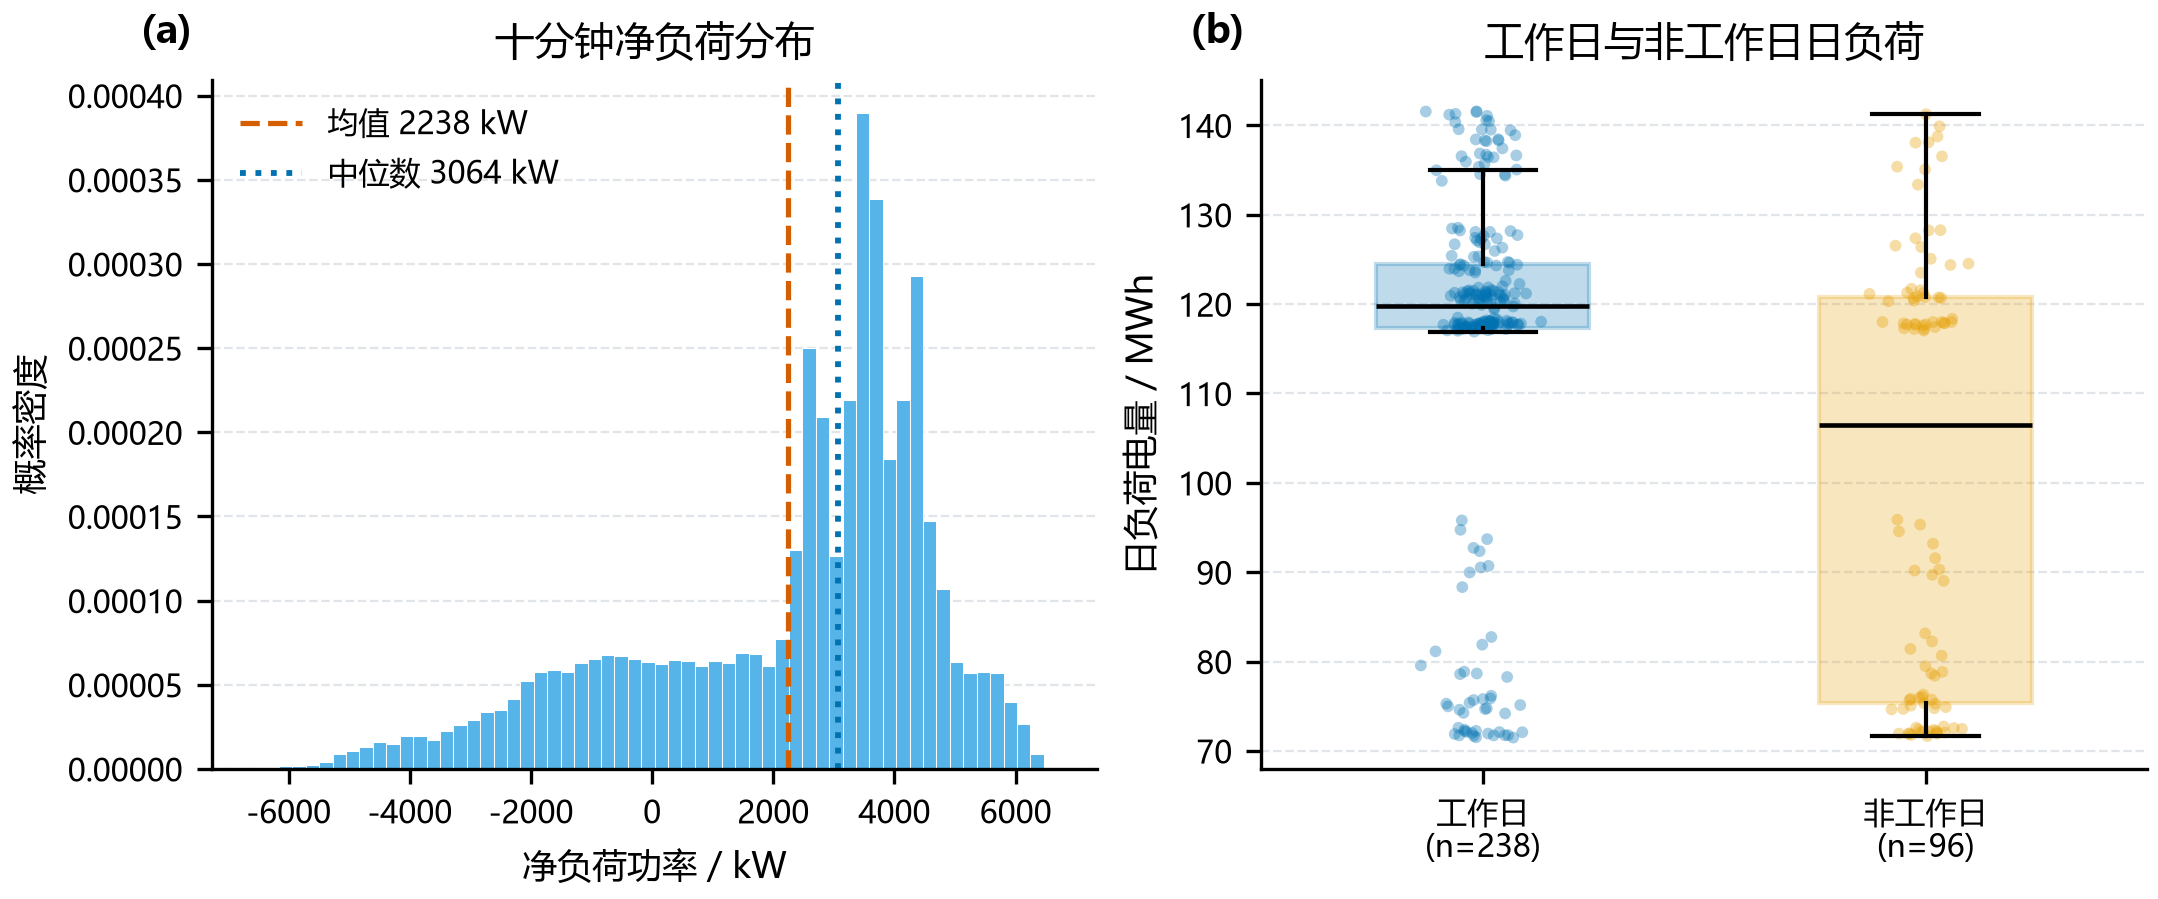
\includegraphics[width=0.94\textwidth]{图3_净负荷分布与工作日差异.png}
    \caption{净负荷分布与工作日差异}
    \label{fig:data-netload-workday}
\end{figure}

月度日均净负荷在5月约38.28 MWh，而12月升至76.26 MWh，反映夏季光伏和冬季供需结构的共同变化。逐时相关系数中，光伏与净负荷为$-0.885$，波动电价与净负荷为0.262，负荷与电价为0.506。图\ref{fig:data-month-corr}说明仅使用全局均值会掩盖季节和日内关系，因此预测器必须在时间顺序内动态更新。

\begin{figure}[htbp]
    \centering
    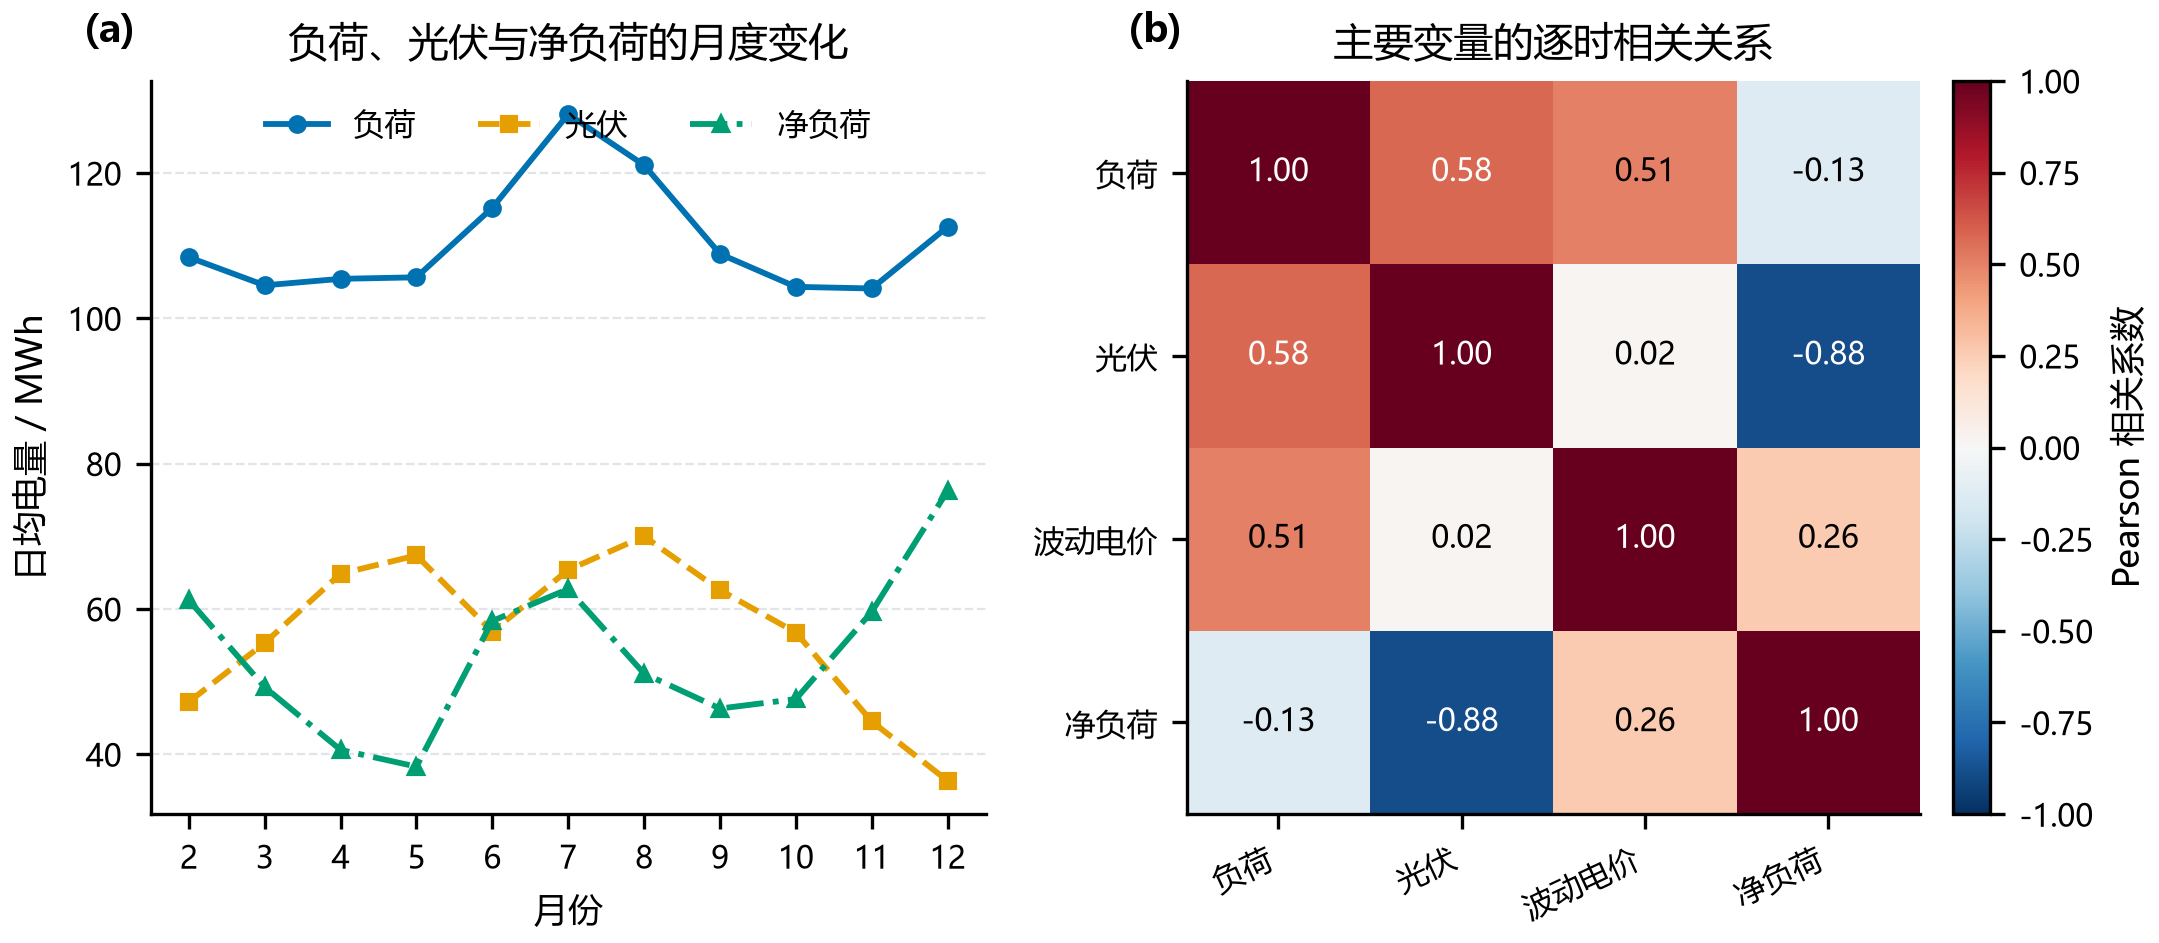
\includegraphics[width=0.94\textwidth]{图4_主要变量月度变化与相关关系.png}
    \caption{主要变量月度变化与相关关系}
    \label{fig:data-month-corr}
\end{figure}

\subsection{净负荷及时序特征}

定义交流侧净负荷电量为
\begin{equation}
n^{\mathrm{act}}_{d,t}=l^{\mathrm{act}}_{d,t}-p^{\mathrm{act}}_{d,t}.
\label{eq:netload}
\end{equation}
当$n^{\mathrm{act}}_{d,t}>0$时，负荷超过光伏，需要由外网或储能放电补足；当其小于0时，存在充电或弃光空间。直接对式\ref{eq:netload}预测能够保留同一历史日中负荷与光伏的配对关系，避免把两个边际分位数拼接成并未共同出现过的极端净负荷。

预处理阶段构造日内和周内周期变量
\begin{equation}
\sin\frac{2\pi t}{144},\quad \cos\frac{2\pi t}{144},\quad
\sin\frac{2\pi \omega_d}{7},\quad \cos\frac{2\pi \omega_d}{7},
\label{eq:time-features}
\end{equation}
其中$\omega_d$为星期序号；同时保留同一时刻的1日、7日滞后及近7日滚动均值作为审计特征。正式预测并未把这些变量全部塞入黑箱回归：问题二明确使用近7日净负荷形状、星期类型和时间衰减选择相似日；问题三的负荷基线使用近56日同星期中位数，并用最近12个已观测时段的偏差作指数衰减校正。这样既利用周期性，也能清楚追溯每项信息的可用时刻。

距离计算中的标准化参数仅用1月1日至31日的4464条记录估计：负荷均值4725.77 kW、标准差1450.45 kW，光伏均值1589.18 kW、标准差2247.01 kW，价格均值0.8596元/kWh、标准差0.3745元/kWh。标准化只用于距离比较，优化目标和物理约束仍使用原始单位。

\subsection{相似日与动态净负荷分位数构建}

对待预测日$d$，只在其前60天中选择候选日；若同星期样本足够，优先保留同星期日期，否则退化为全部历史日期。以过去7日配对净负荷的均值曲线$\bar n^{(7)}_{d,t}$为参考，历史日$j$的距离为
\begin{equation}
D_{d,j}=\sqrt{\frac{1}{144}\sum_{t=1}^{144}
\left(\frac{n^{\mathrm{act}}_{j,t}-\bar n^{(7)}_{d,t}}{\sigma_n}\right)^2}
+0.15\frac{d-j}{60},
\label{eq:similar-score}
\end{equation}
其中$\sigma_n=\max\{\mathrm{std}(n),1\}$。选取距离最小的20天，对同一时段的配对净负荷取条件分位数：
\begin{equation}
\widehat n_{d,t\mid0}(\alpha)=Q_{\alpha}\!\left(
\left\{n^{\mathrm{act}}_{j,t}:j\in\mathcal S_d\right\}\right),
\quad \alpha\in\{0.50,0.55,\ldots,0.95\}.
\label{eq:net-quantile}
\end{equation}

分位数不是固定指定，而是用最近14个已执行历史日的运行费用滚动选择。候选分位数的得分为
\begin{equation}
J_d(\alpha)=\overline C_d(\alpha)+0.2\,\mathrm{CVaR}_{0.95,d}(\alpha)
+0.02\,\overline C_d(\alpha)\frac{|\alpha-\alpha_{d-1}|}{0.05}.
\label{eq:quantile-score}
\end{equation}
第一项衡量平均运行费用，第二项抑制尾部高成本，第三项避免分位数无意义频繁跳变。当有效验证日不足14天时使用默认0.80；当天执行结束后才把该日所有候选分位数的反事实费用加入历史。因而式\ref{eq:quantile-score}的选择严格因果，也与后续调度的经济目标保持一致。

2021年发表于《电力系统保护与控制》的研究利用条件风险价值量化微电网不确定性风险，为按照尾部运行成本选择预测分位数提供了方法参考\cite{chen2021cvar}。

\subsection{因果性控制与预处理小结}

全部预测均遵守“先发布、后决策、再观测”的顺序：相似日集合不含当天及未来日期；分位数验证只用已执行日；四时点光伏预测只使用最近一次正式发布值；日内偏差校正只读取当前时点之前的实际观测；标准化参数固定在正式评价期以前。预处理最终形成了无重复时间键、量纲一致、保留真实峰值且可按信息时点回放的数据集，为四个问题共用的MILP物理层和严格因果回测提供基础。

\section{问题一：确定性单日储能调度}

\subsection{信息条件与决策变量}

问题一在一天开始时已知附件1中的144个负荷、光伏预测和固定分时电价。模型分别设置购电量$g_t$、交流侧充电量$c_t$、交流侧放电量$b_t$、弃光量$w_t$和电池内部状态$s_t$。购电、充电和放电不能合并为一个带符号变量：购电承担外部费用，充电改变未来可用能量，放电受既有SOC限制；若混为一项，将无法分别施加非负、效率和互斥约束。

图\ref{fig:q1-solution-flow}概括问题一从目标与约束识别、数据预处理、模型建立与两阶段求解，到结果检验和结论输出的完整解题思路。

\begin{figure}[H]
    \centering
    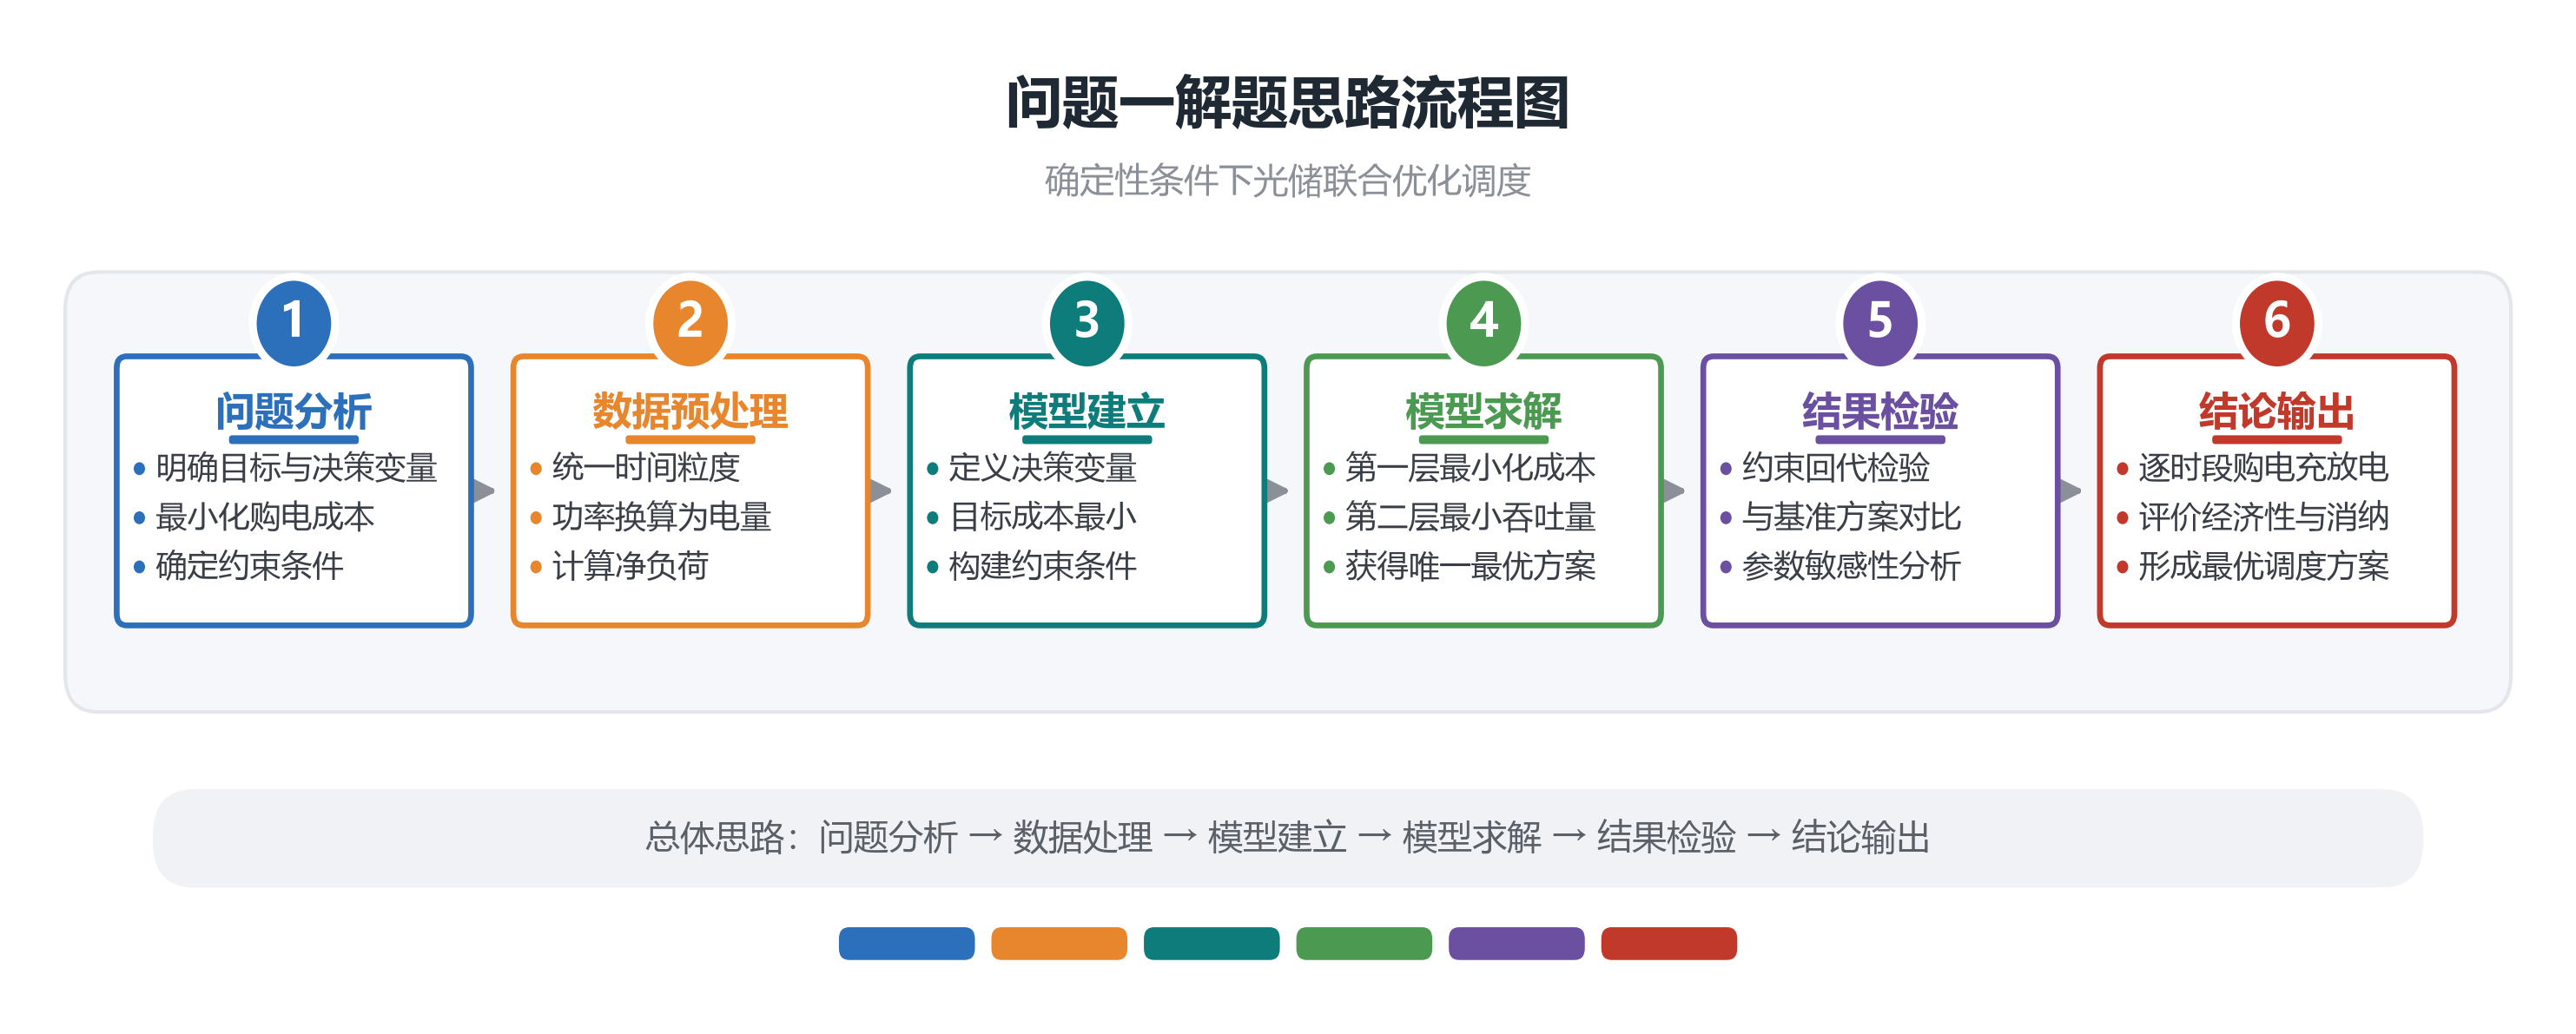
\includegraphics[width=0.98\textwidth]{图5_问题一解题思路流程图.png}
    \caption{问题一解题思路流程图}
    \label{fig:q1-solution-flow}
\end{figure}

\subsection{供需平衡与储能物理约束}

交流侧每个时段满足
\begin{equation}
g_t+p^{\mathrm{for}}_t+b_t=l^{\mathrm{for}}_t+c_t+w_t.
\label{eq:q1-balance}
\end{equation}
式\ref{eq:q1-balance}把购电、光伏和储能放电作为供给，把负荷、充电和剩余电量作为去向。由于$c_t$和$b_t$已经是交流侧电量，平衡式中不再乘效率；若在此再次折算，会重复计算损耗。电池内部状态递推为
\begin{equation}
s_t=s_{t-1}+\eta_c c_t-\frac{b_t}{\eta_b},
\qquad E^{\min}\le s_t\le E^{\max}.
\label{eq:soc-transition}
\end{equation}
充入$c_t$后只有$\eta_c c_t$留在电池内部；向交流侧输出$b_t$则需从电池内部取出$b_t/\eta_b$。因此总充电量大于总放电量是效率损耗和终端闭合共同作用的正常结果，并非能量不守恒。

有限功率和充放电互斥约束为
\begin{equation}
\begin{aligned}
0\le c_t&\le P^{\max}\Delta t\,z^c_t,\\
0\le b_t&\le P^{\max}\Delta t\,z^b_t,\\
z^c_t+z^b_t&\le1,\qquad z^c_t,z^b_t\in\{0,1\}.
\end{aligned}
\label{eq:binary-operation}
\end{equation}
二元变量使模型成为混合整数线性规划，并从物理上排除同一时段的无效同时充放电。所有变量非负且不设置售电变量；$w_t$保留了光伏富余或已购电未消纳的可行出口。问题一按题意取$s_0=s_{144}=6000$ kWh，防止模型通过耗尽电池虚减当日成本。

2020年发表于《浙江电力》的研究通过分段线性化将源--车--储微电网调度模型转化为混合整数线性规划，为含连续能量变量和离散运行状态的统一求解提供了参考\cite{chen2020milp}。

\subsection{两阶段词典序目标与求解}

第一层严格最小化题目规定的购电费用：
\begin{equation}
C_1^*=\min\sum_{t=1}^{144}\pi_t g_t.
\label{eq:q1-primary}
\end{equation}
获得$C_1^*$后，在$\sum_t\pi_tg_t\le C_1^*+\varepsilon_C$约束下求解第二层
\begin{equation}
\min\sum_{t=1}^{144}(c_t+b_t),\qquad
\varepsilon_C=\max\{10^{-5},10^{-9}|C_1^*|\}.
\label{eq:q1-secondary}
\end{equation}
式\ref{eq:q1-secondary}只在同成本或数值容差内近同成本的方案中减少吞吐量，消除无效循环；它不是将0.005元/kWh惩罚混入经济目标的普通加权法。两层均调用SciPy的\texttt{milp}接口，由HiGHS求解器求解，MIP相对间隙设为$10^{-9}$。问题一的完整建模、求解与检验步骤已由图\ref{fig:q1-solution-flow}统一概括。

\subsection{调度结果与典型时段}

表\ref{tab:q1-main-results}给出单日总体结果。储能使购电费用由48052.05元降至35126.95元，节约12925.10元、降幅26.90\%。购电量反而只减少2307.24 kWh，而充电量比放电量多3940.73 kWh，说明收益主要来自把低价购电和午间富余光伏转移到高价时段，而不是无损地凭空减少能量。弃光为0表明储能容量与调度时点在该日足以吸收可利用的光伏富余。

\begin{table}[htbp]
\centering
\small
\caption{问题一有无储能的总体结果}\label{tab:q1-main-results}
\begin{tabular}{lrr}
\toprule
指标 & 有储能 & 无储能\\
\midrule
全天购电量/kWh & 59482.6990 & 61789.9354\\
全天购电费用/元 & 35126.9486 & 48052.0466\\
相对无储能节约/元 & 12925.0980 & --\\
相对无储能降幅 & 26.8981\% & --\\
总充电量/kWh & 20740.6660 & --\\
总放电量/kWh & 16799.9395 & --\\
弃光量/kWh & 0.0000 & 0.0000\\
SOC范围/kWh & $[1200,10800]$ & --\\
\bottomrule
\end{tabular}
\end{table}

指定时刻的购电量见表\ref{tab:q1-specified-times}，与结果工作簿逐项一致。10:00和14:00购电量为0，说明光伏及储能能够覆盖负荷；18:00购电量升至636.9826 kWh，反映傍晚光伏下降后净负荷重新上升。

\begin{table}[htbp]
\centering
\small
\caption{问题一指定时刻的最优购电量}\label{tab:q1-specified-times}
\begin{tabular}{crcrcr}
\toprule
时刻 & 购电量/kWh & 时刻 & 购电量/kWh & 时刻 & 购电量/kWh\\
\midrule
10:00 & 0.0000 & 12:00 & 486.4029 & 14:00 & 0.0000\\
16:00 & 394.9315 & 18:00 & 636.9826 & 20:00 & 0.0000\\
\bottomrule
\end{tabular}
\end{table}

按四小时汇总的储能动作见表\ref{tab:q1-fourhour}。0--4时以低价购电充电，4--8时进入集中放电；8--16时同时经历光伏增强和储能补充；16--20时完全不充电并放出5068.69 kWh；20时后利用价格回落恢复终端SOC。

\begin{table}[htbp]
\centering
\small
\caption{问题一各四小时区间的充放电量}\label{tab:q1-fourhour}
\begin{tabular}{crrcrr}
\toprule
区间/h & 充电/kWh & 放电/kWh & 区间/h & 充电/kWh & 放电/kWh\\
\midrule
0--4 & 4500.0000 & 0.0000 & 12--16 & 6119.3685 & 91.1014\\
4--8 & 833.3333 & 5947.4196 & 16--20 & 0.0000 & 5068.6869\\
8--12 & 3954.6308 & 2121.4184 & 20--24 & 5333.3333 & 3571.3132\\
\bottomrule
\end{tabular}
\end{table}

图\ref{fig:q1-soc-actions}给出充放电与SOC的同步变化。SOC始终位于1200--10800 kWh，且24:00回到6000 kWh；没有任何同时充放电时段。图\ref{fig:q1-storage-compare}进一步显示，有储能方案并非在所有时段都减少购电：低价阶段主动多购，高价阶段显著少购，费用节约来自跨时段价差、光伏消纳和储能效率三者的平衡。

\begin{figure}[htbp]
    \centering
    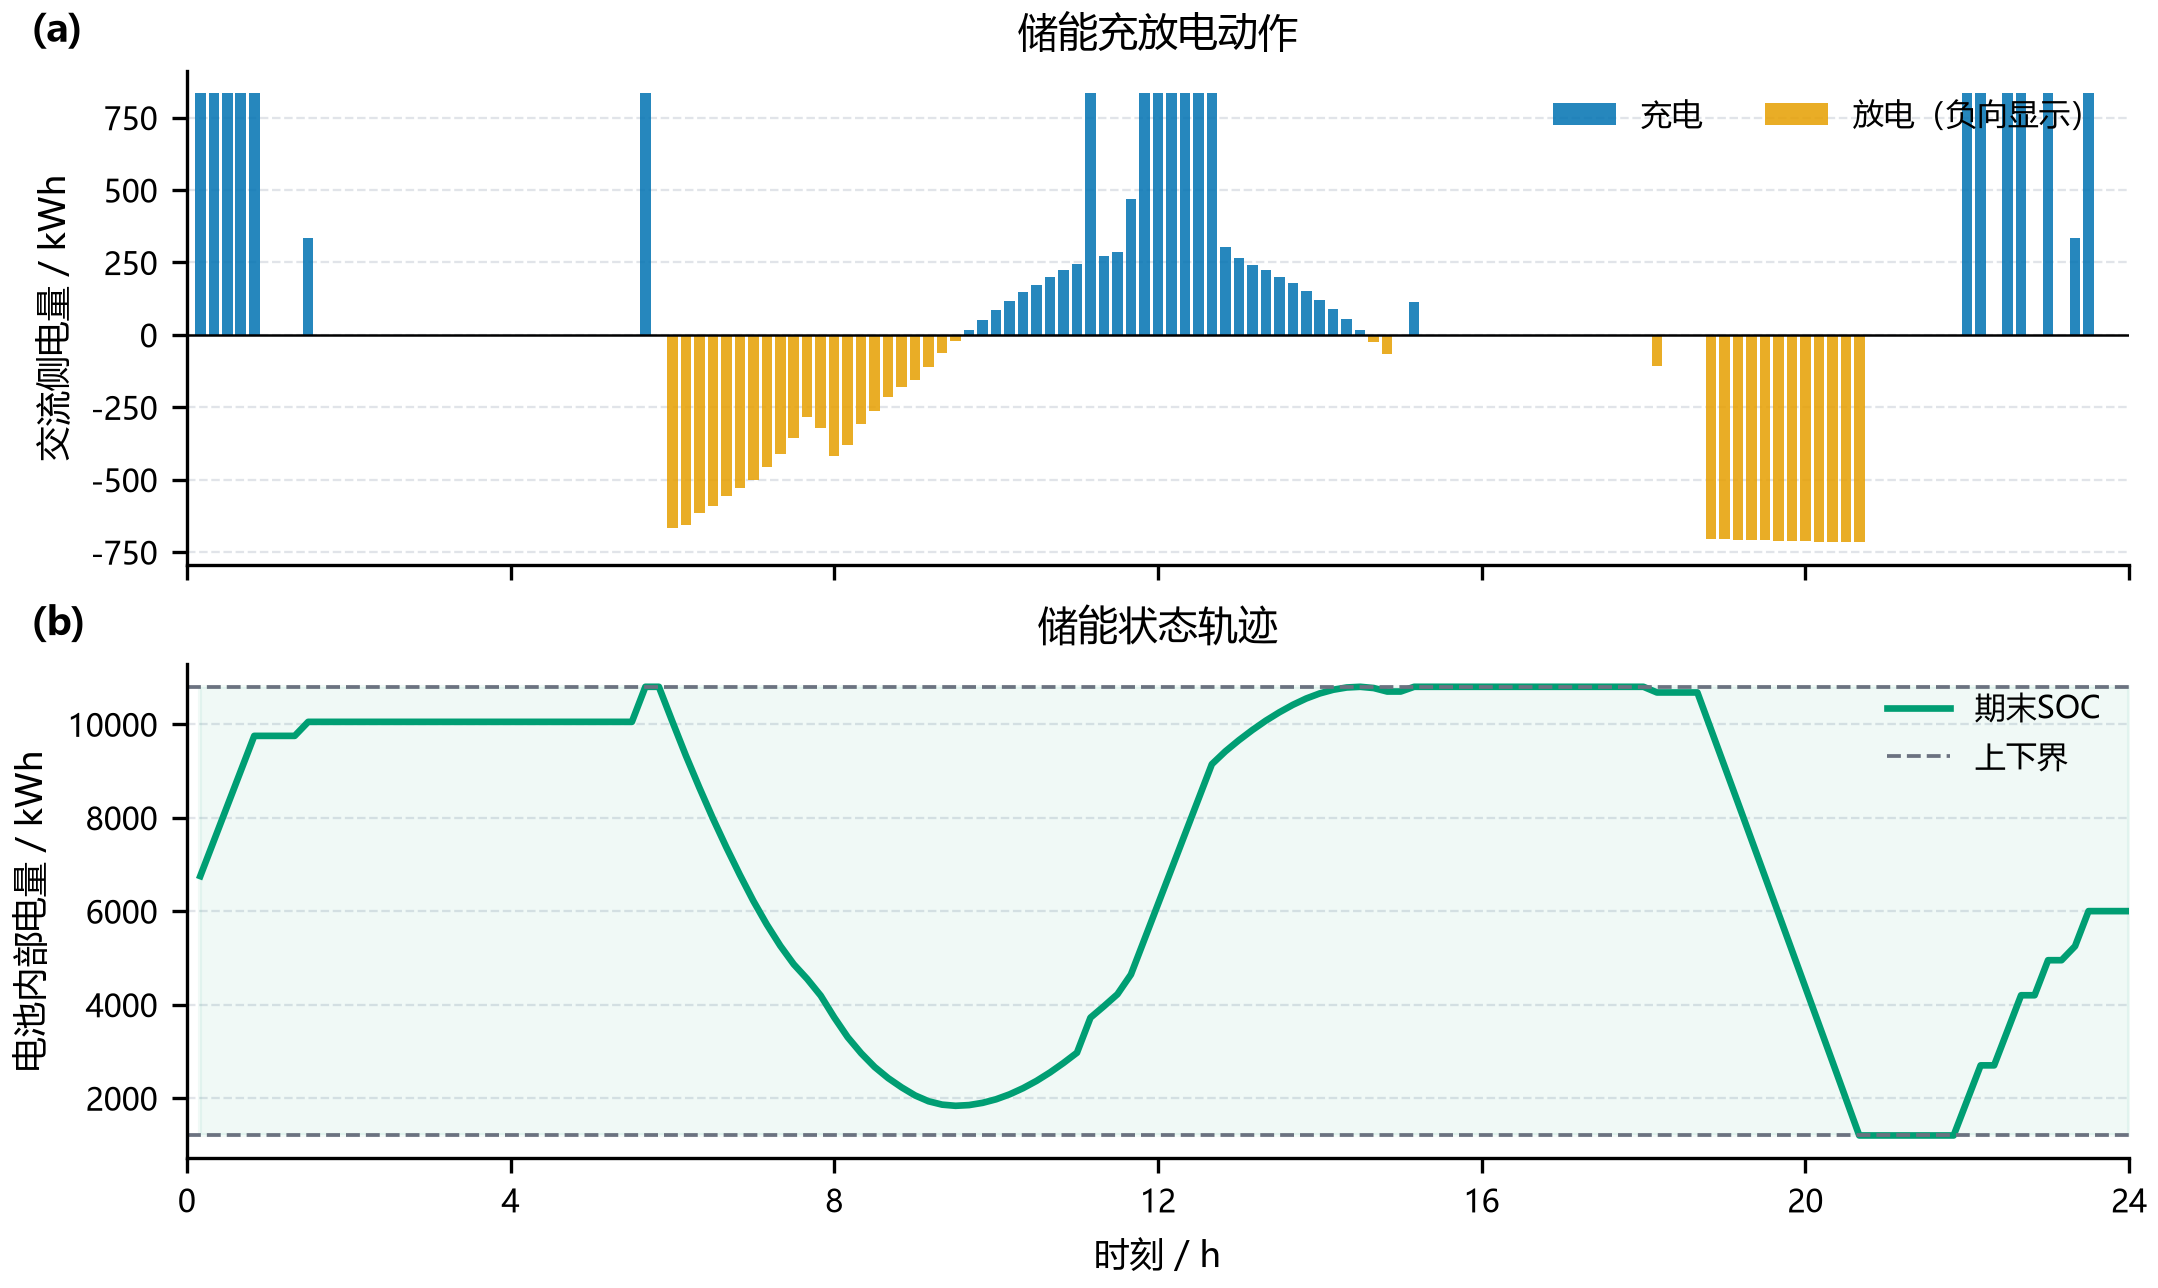
\includegraphics[width=0.92\textwidth]{图6_问题一储能状态与充放电行为.png}
    \caption{问题一储能状态与充放电行为}
    \label{fig:q1-soc-actions}
\end{figure}

\begin{figure}[htbp]
    \centering
    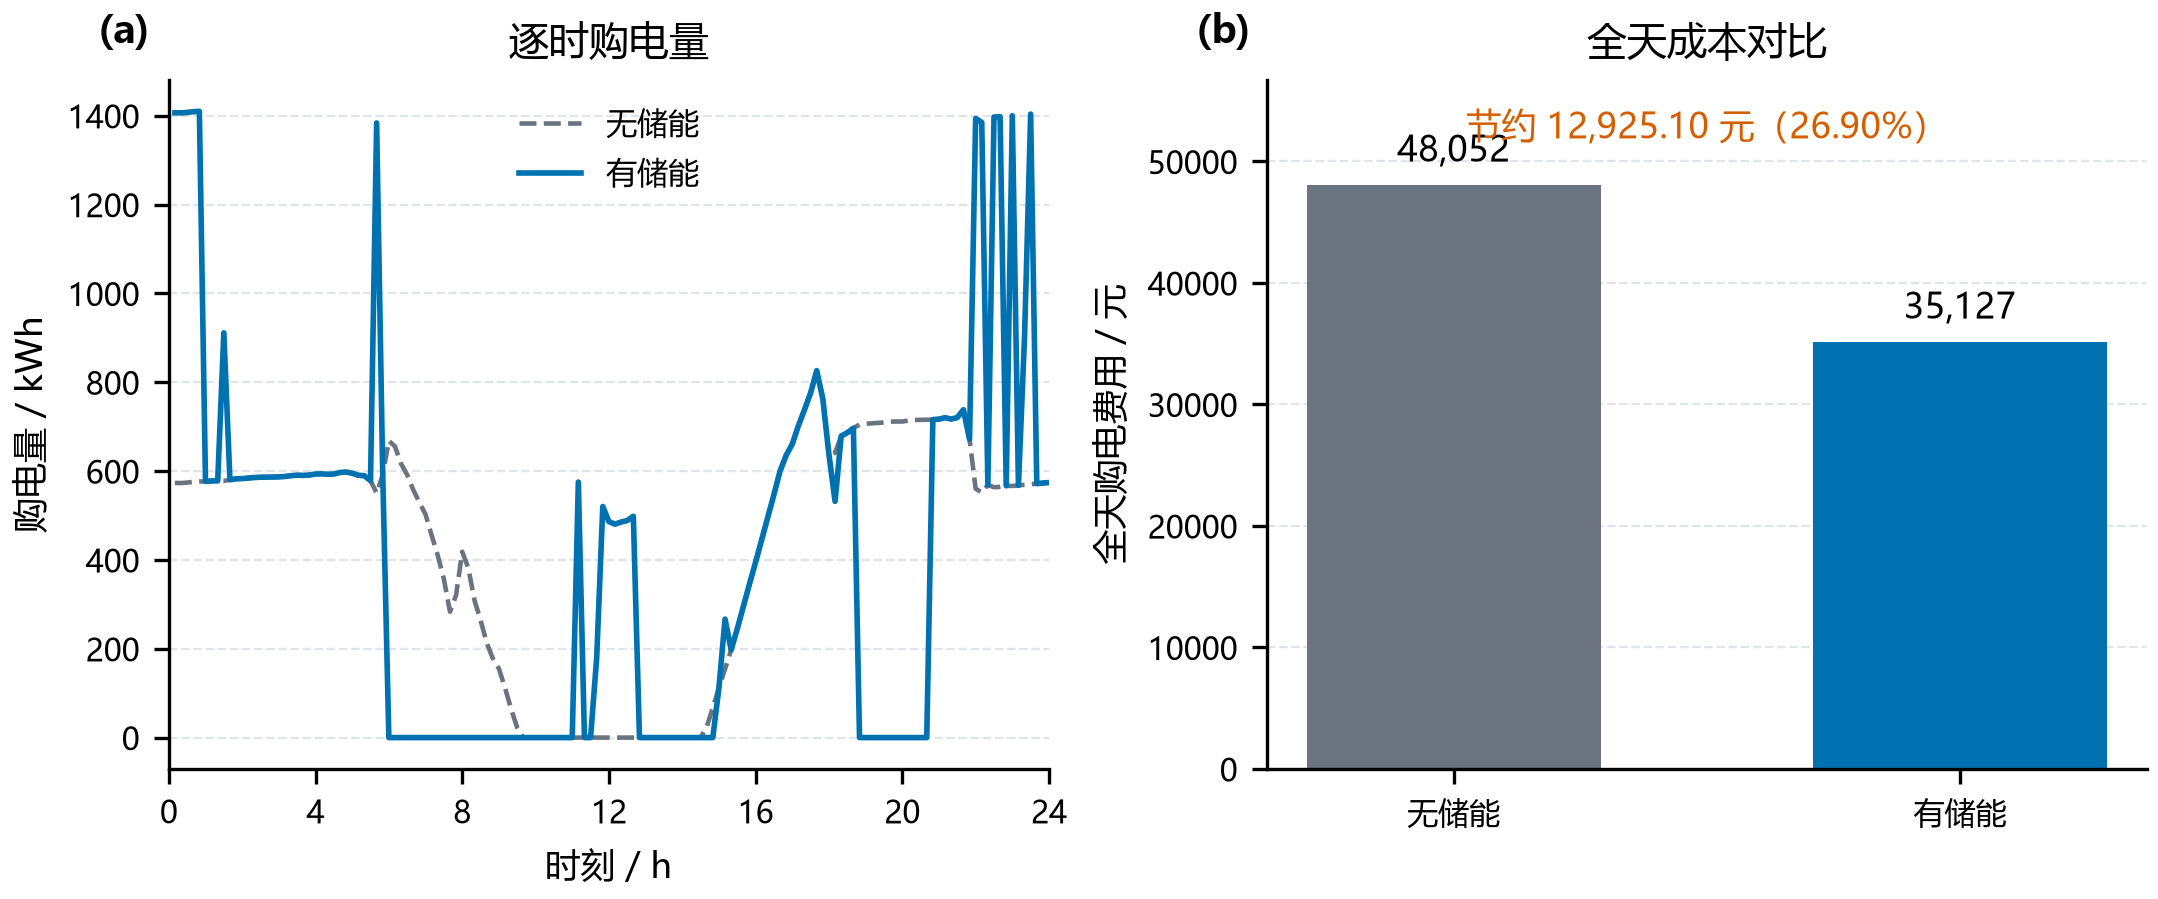
\includegraphics[width=0.92\textwidth]{图7_问题一有无储能购电策略对比.png}
    \caption{问题一有无储能购电策略对比}
    \label{fig:q1-storage-compare}
\end{figure}

\subsection{效率敏感性与本问小结}

图\ref{fig:q1-efficiency}将单程效率从0.80提高到1.00。往返效率由64\%升至100\%时，最优购电费用由38223.65元降至32377.09元；基准往返效率81\%对应35126.95元。曲线单调下降，说明结论符合损耗机理，但节费幅度依赖电池效率，不能把基准收益直接外推到性能较差的储能设备。

\begin{figure}[htbp]
    \centering
    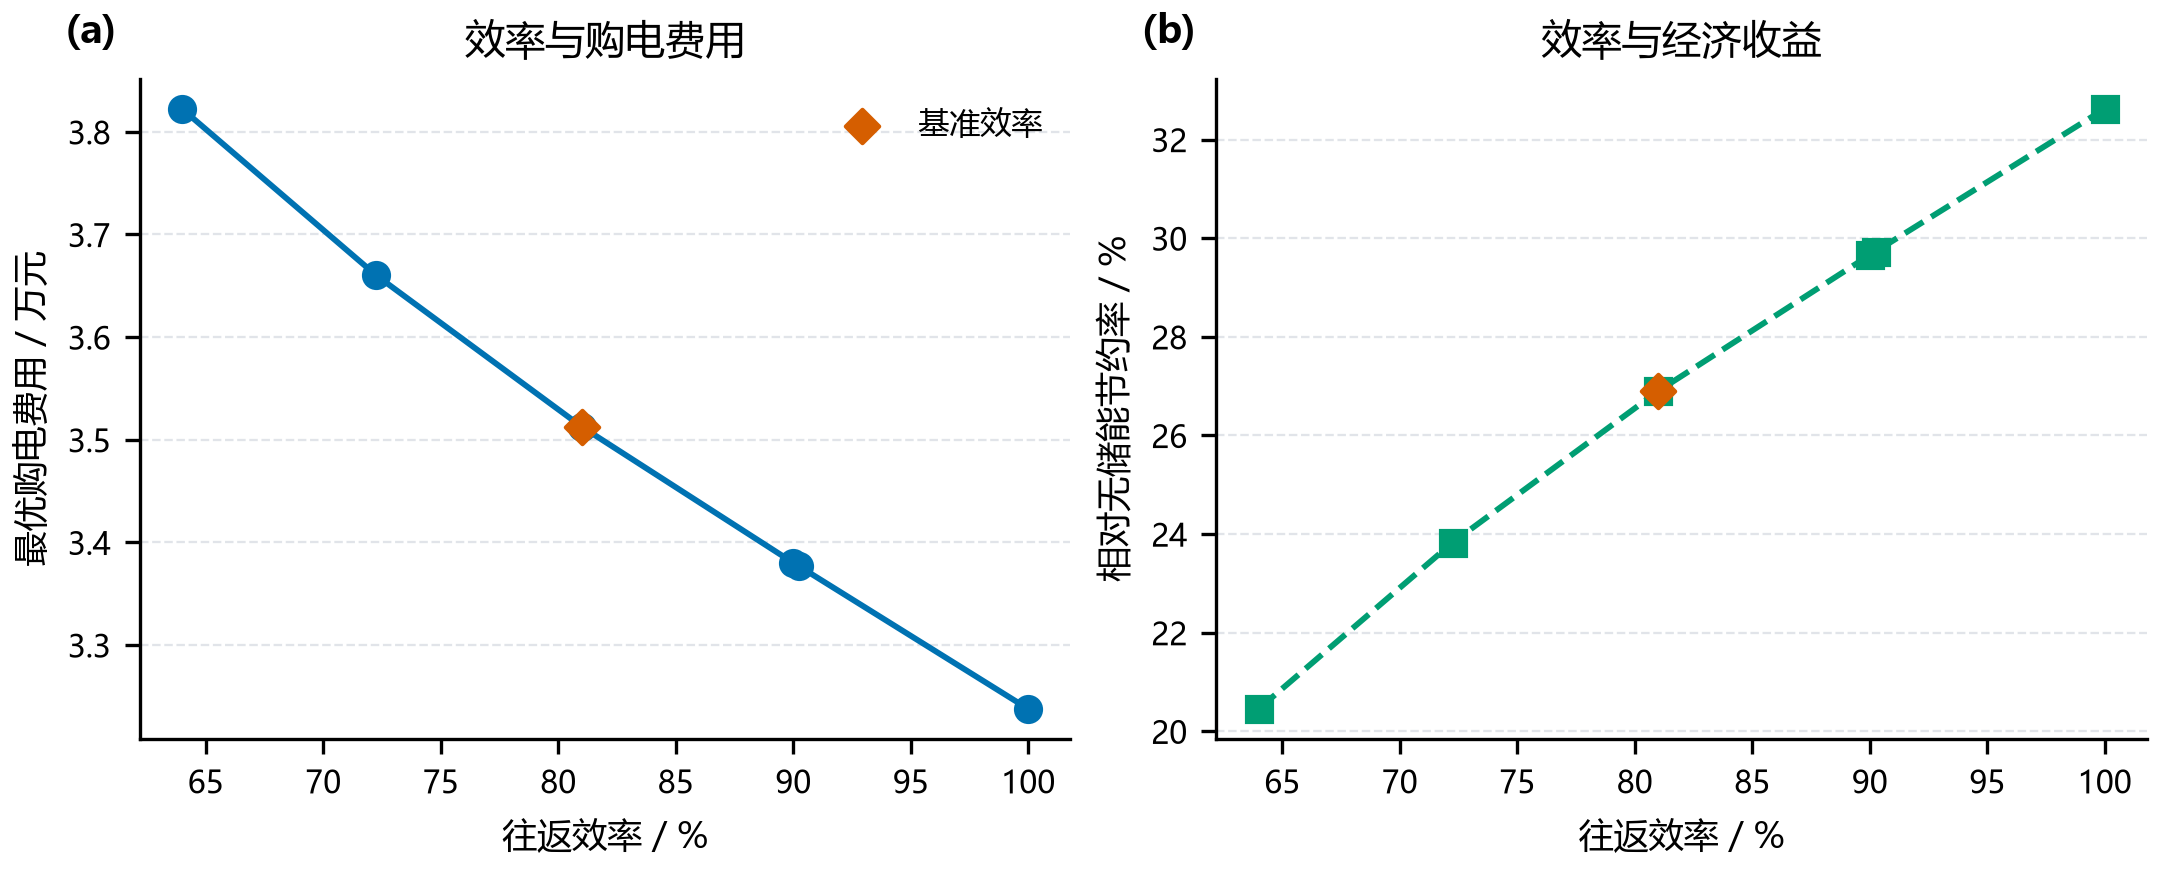
\includegraphics[width=0.91\textwidth]{图8_问题一储能效率敏感性.png}
    \caption{问题一储能效率敏感性}
    \label{fig:q1-efficiency}
\end{figure}

综上，问题一的确定性MILP在单日终端SOC闭合条件下实现了低价充电、光伏富余吸收和高价放电，成本较无储能下降26.90\%。二元互斥和第二层吞吐量最小化共同保证了结果既满足物理可行性，又不依赖同成本循环。

\section{问题二：预测偏差下的日前计划}

\subsection{预测误差的经济机制与信息条件}

问题二每天0:00制定次日144个时段的购电与储能计划，此时只能使用此前已观测的负荷、光伏和历史运行费用。计划净负荷偏低会造成实际供电缺口，并按当时电价的5倍紧急购电；计划偏高则已购电无法退款，只能用于负荷、充电或记为剩余电量。因此，统计意义上最接近均值的点预测未必带来最低运行成本，预测器需要在计划冗余和高价缺口之间作经济权衡。

图\ref{fig:q2-solution-flow}展示问题二围绕因果预测、分位数选参、日前计划、实时补救、执行结算及逐日回代检验展开的两阶段求解流程。

\begin{figure}[H]
    \centering
    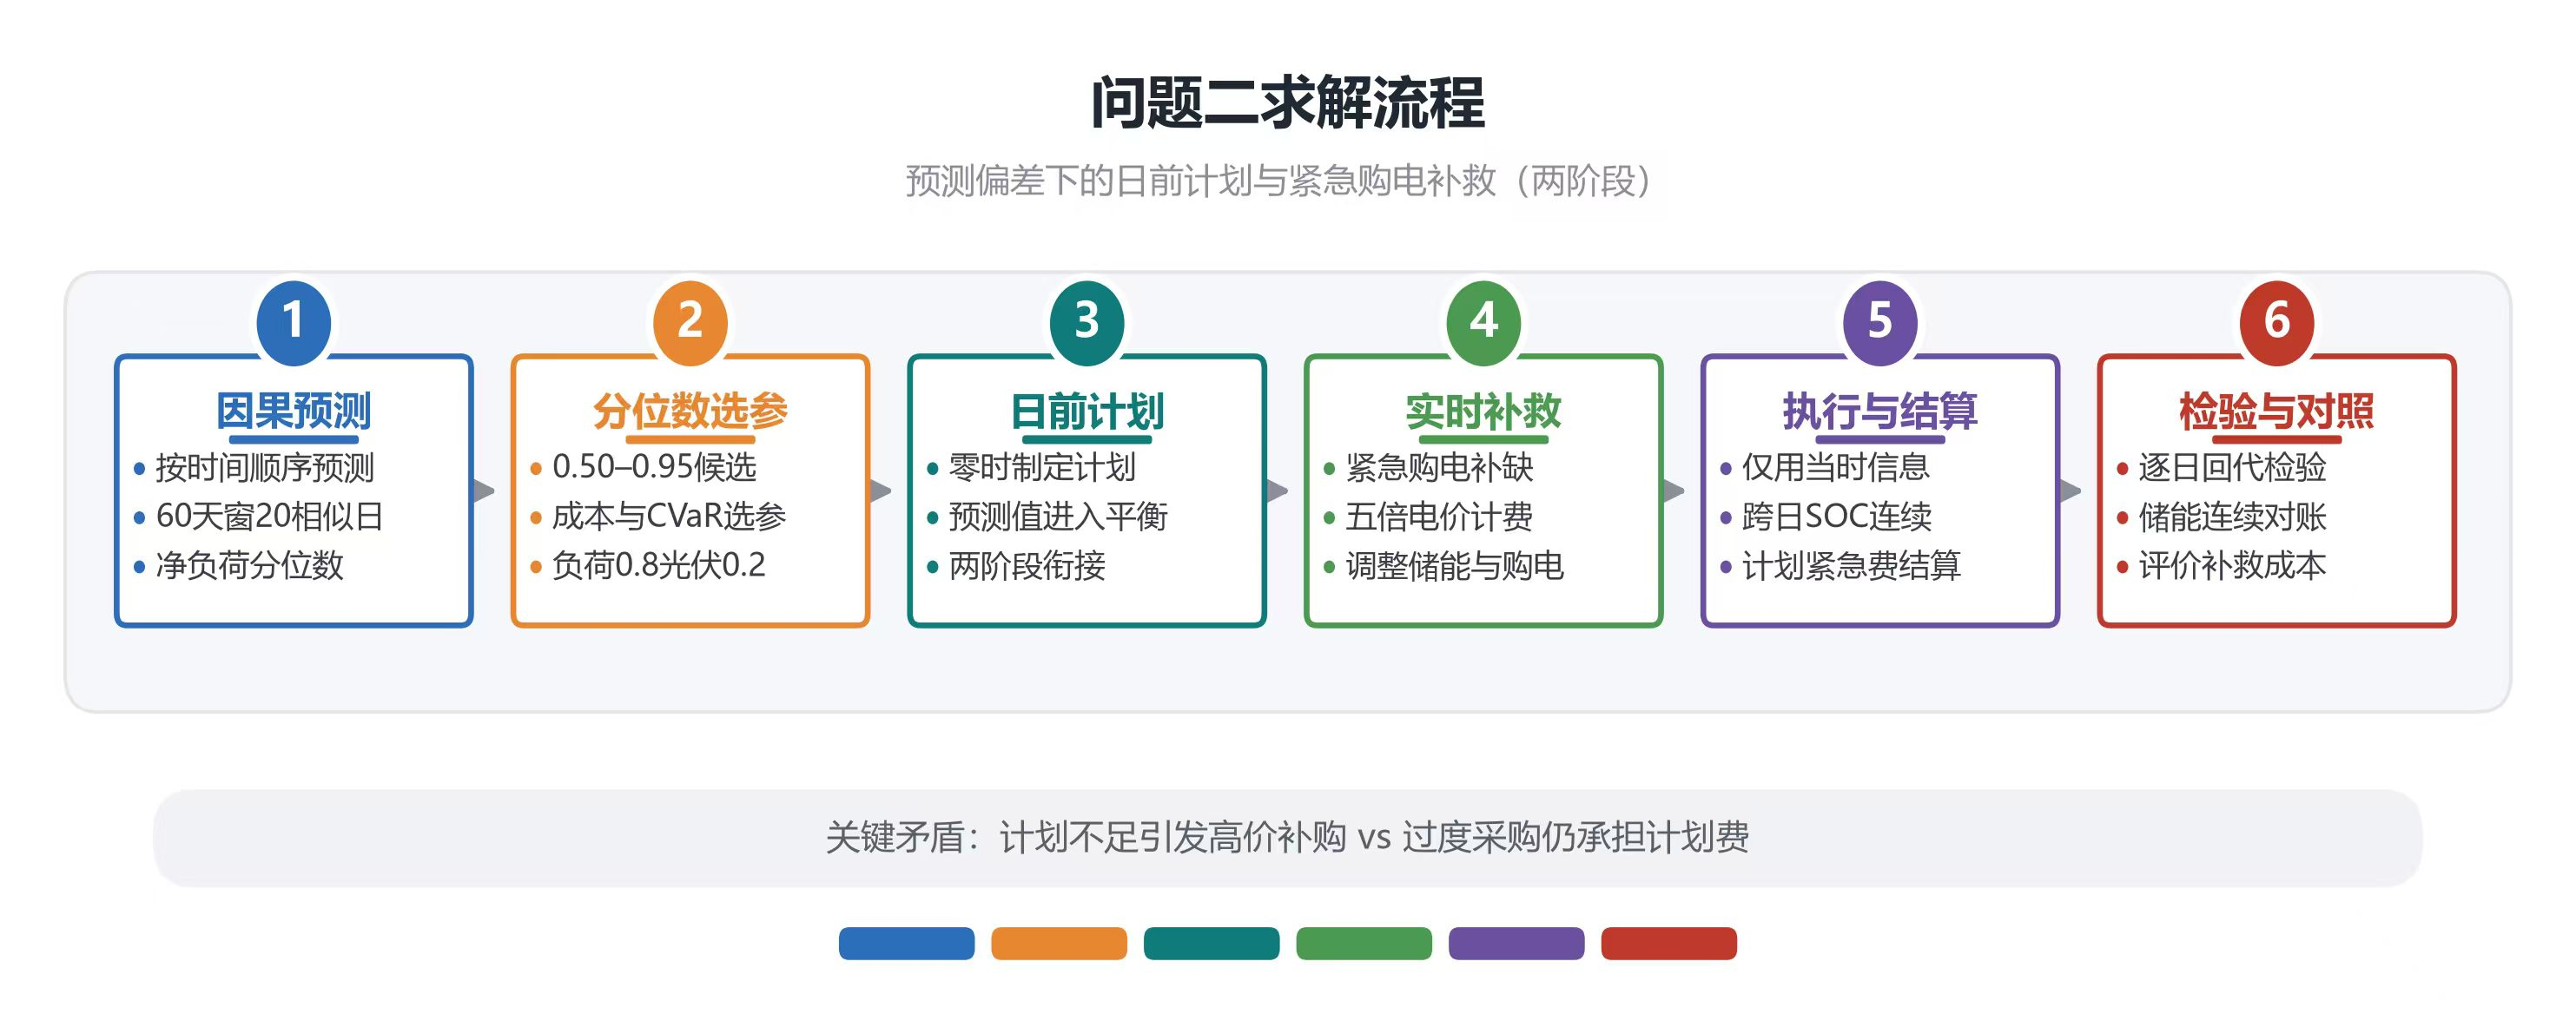
\includegraphics[width=0.98\textwidth]{图9_问题二求解流程图.jpg}
    \caption{问题二求解流程图}
    \label{fig:q2-solution-flow}
\end{figure}

\subsection{动态净负荷分位数预测}

问题二采用第5节式\ref{eq:net-quantile}和式\ref{eq:quantile-score}，直接对同一历史日的“负荷减光伏”序列取动态条件分位数。训练窗口60天、相似日20天、验证窗口14天，候选分位数为0.50--0.95、步长0.05。该方法与“负荷固定0.80分位数减光伏固定0.20分位数”不同：后者把两个可能来自不同日期的边际尾部拼接，既破坏负荷和光伏的相关结构，也无法随价格和历史缺口成本调整风险水平。

2025年发表于《中国电力》的研究利用共形分位数回归构造光伏功率预测区间，说明分位数方法能够在不预设固定概率分布的情况下刻画光伏预测不确定性\cite{gui2025quantile}。

图\ref{fig:q2-forecast-error}给出按结果文件中的当日分位数重新构造的代表日预测和正式评价期误差分布。误差定义为实际净负荷减日前预测，正误差意味着潜在缺口。分布存在双侧尾部，说明单一固定裕度无法覆盖全年季节变化。

\begin{figure}[htbp]
    \centering
    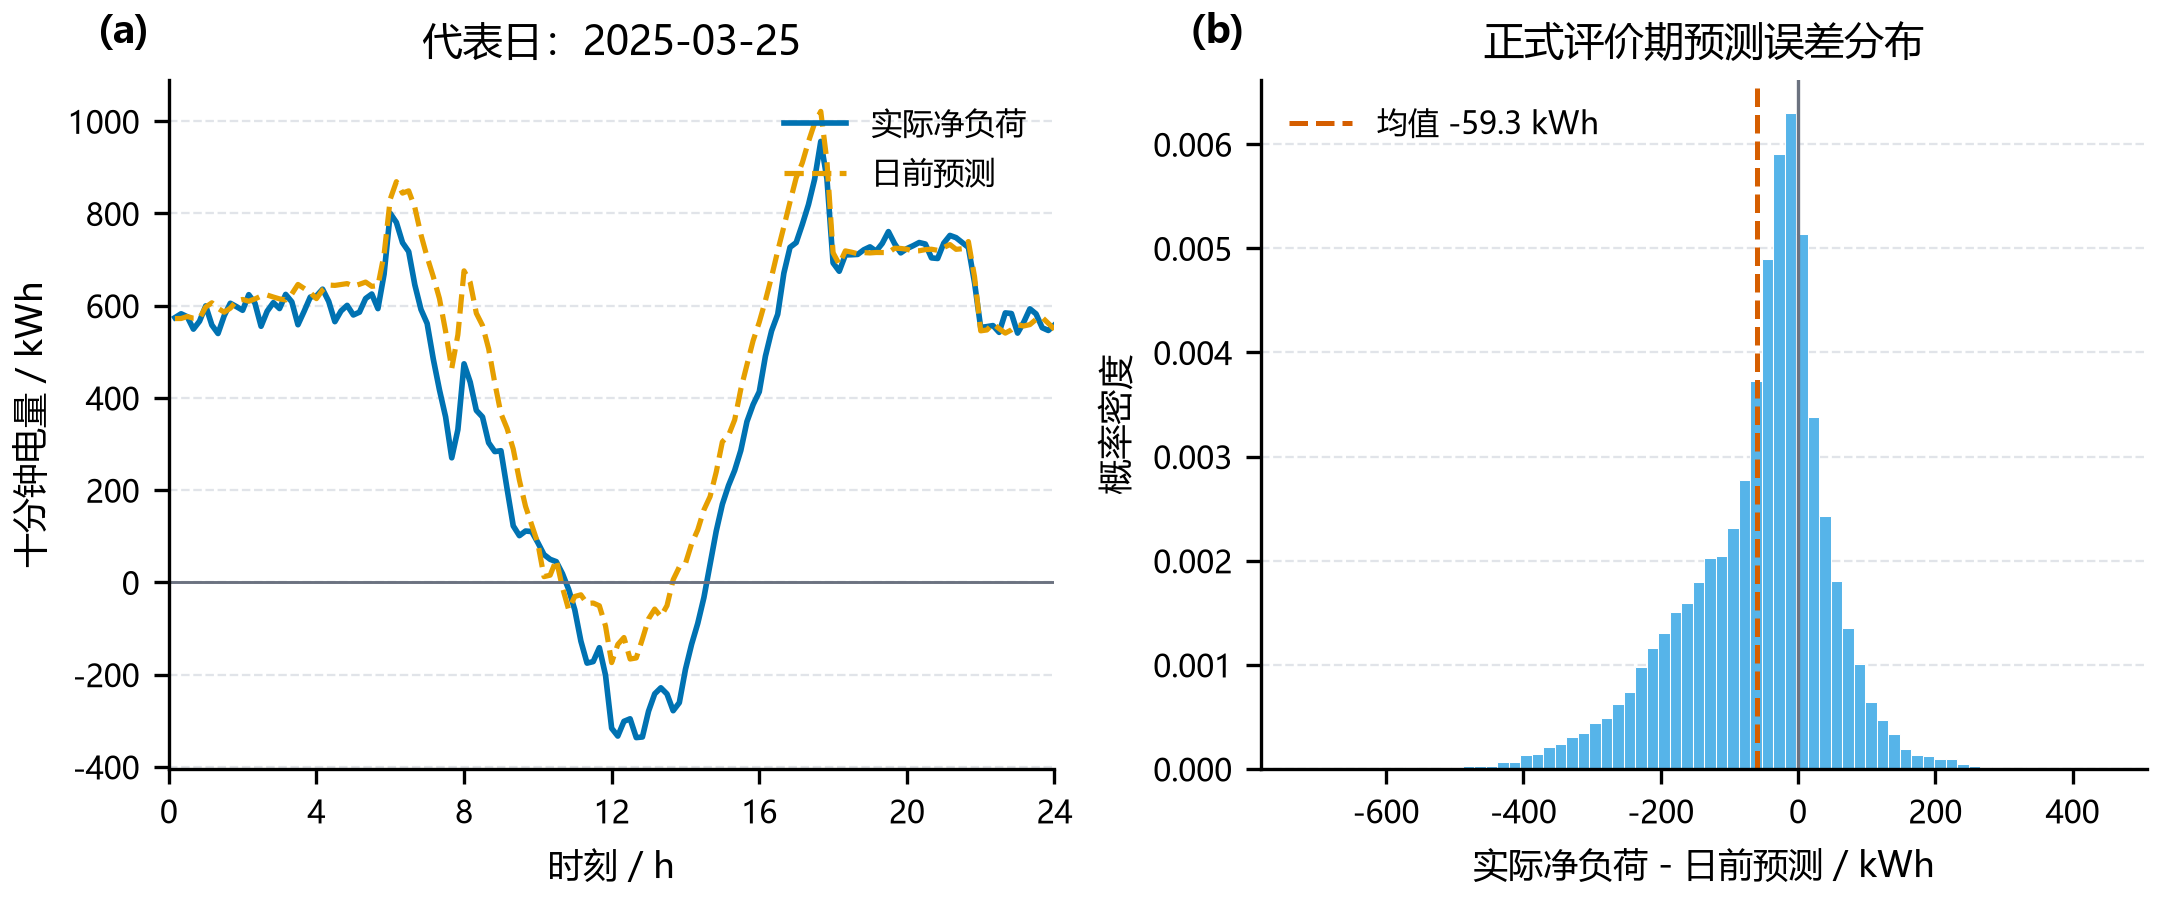
\includegraphics[width=0.93\textwidth]{图10_实际净负荷与日前预测误差.png}
    \caption{实际净负荷与日前预测误差}
    \label{fig:q2-forecast-error}
\end{figure}

\subsection{日前MILP与实际执行机制}

把预测净负荷分解为$\widehat l_{d,t\mid0}=\max(\widehat n_{d,t\mid0},0)$与$\widehat p_{d,t\mid0}=\max(-\widehat n_{d,t\mid0},0)$，日前计划仍使用与问题一相同的混合整数物理层。等价的净负荷平衡为
\begin{equation}
g^0_{d,t}+b^0_{d,t}=\widehat n_{d,t\mid0}+c^0_{d,t}+w^0_{d,t}.
\label{eq:q2-plan-balance}
\end{equation}
模型保留有限功率、充放电二元互斥和式\ref{eq:soc-transition}。不同于问题一，问题二不要求每天日末SOC回到当天日初；前一日实际期末状态直接作为下一日初值，只在整个365日计算区间末端回到6000 kWh。这允许电量跨日传递，也避免把人为的每日闭合误写为现实运行规则。

执行时冻结日前的$g^0,c^0,b^0$，用实际负荷和光伏计算
\begin{equation}
e_{d,t}=\max\{l^{\mathrm{act}}_{d,t}+c^0_{d,t}-g^0_{d,t}-p^{\mathrm{act}}_{d,t}-b^0_{d,t},0\},
\label{eq:q2-emergency}
\end{equation}
剩余电量则取同一平衡差的正向部分。正式成本为
\begin{equation}
C^{\mathrm{tot}}_2=\sum_{d,t}\left(\pi_tg^0_{d,t}+5\pi_t e_{d,t}\right).
\label{eq:q2-total-cost}
\end{equation}
由于第二层仍仅在第一层最优费用容差内最小化$\sum(c+b)$，式\ref{eq:q2-total-cost}没有混入人为吞吐惩罚。

\subsection{全年滚动求解流程}

算法从1月1日$s=6000$ kWh开始：每天先根据截至前一天的历史费用选择$\alpha_d$，再生成净负荷预测并求解两阶段MILP；随后以实际负荷、实际光伏执行整日计划，计算紧急购电和剩余电量，写回实际期末SOC；最后才更新每个候选分位数的历史反事实费用。1月结果用于状态和选择历史的连续初始化，正式评价只统计2月1日至12月31日。该顺序保证任何一天的分位数、购电计划和SOC都不含未来实际值。

\subsection{成本、风险与分位数结果}

问题二正式评价期结果见表\ref{tab:q2-results}。计划购电2270.23万kWh，紧急购电62.28万kWh；紧急购电量只占实际外部购电量的2.67\%，但因价格为5倍，费用占总成本15.16\%。这说明少量正向预测误差即可产生显著经济损失，分位数选择不能只追求对称误差最小。

\begin{table}[htbp]
\centering
\small
\caption{问题二正式评价期的购电、储能与成本结果}\label{tab:q2-results}
\begin{tabular}{lr@{\qquad}lr}
\toprule
指标 & 数值 & 指标 & 数值\\
\midrule
计划购电量/kWh & 22702253.66 & 计划购电费/元 & 13924597.96\\
紧急购电量/kWh & 622766.43 & 紧急购电费/元 & 2488920.11\\
剩余电量/kWh & 4058140.12 & 总成本/元 & 16413518.08\\
充电量/kWh & 6965107.81 & 放电量/kWh & 5637417.33\\
SOC范围/kWh & $[1200,10800]$ & 正式评价天数 & 334\\
\bottomrule
\end{tabular}
\end{table}

表\ref{tab:q2-alpha}显示动态分位数并非长期停留在单一高位：平均值为0.8076，中位数为0.85，全年发生11次切换；0.50和0.95分别使用61天和125天。较高分位数增加计划裕度但也可能扩大剩余电量，较低分位数减少计划采购却暴露于高价应急风险，最优方向取决于近期负荷、光伏、价格和尾部成本的联合表现。

\begin{table}[htbp]
\centering
\small
\caption{问题二动态净负荷分位数的使用天数}\label{tab:q2-alpha}
\begin{tabular}{crrrrrrrr}
\toprule
分位数 & 0.50 & 0.55 & 0.60 & 0.65 & 0.80 & 0.85 & 0.90 & 0.95\\
\midrule
天数 & 61 & 7 & 3 & 3 & 47 & 78 & 10 & 125\\
\bottomrule
\end{tabular}
\end{table}

图\ref{fig:q2-alpha-emergency}把每日选择与月度紧急购电并列展示。6月和12月的紧急购电较高，但分位数变化并非与单月缺口机械同向，因为选择得分使用过去14天的平均成本、尾部成本和切换惩罚，而非事后读取当月结果。

\begin{figure}[htbp]
    \centering
    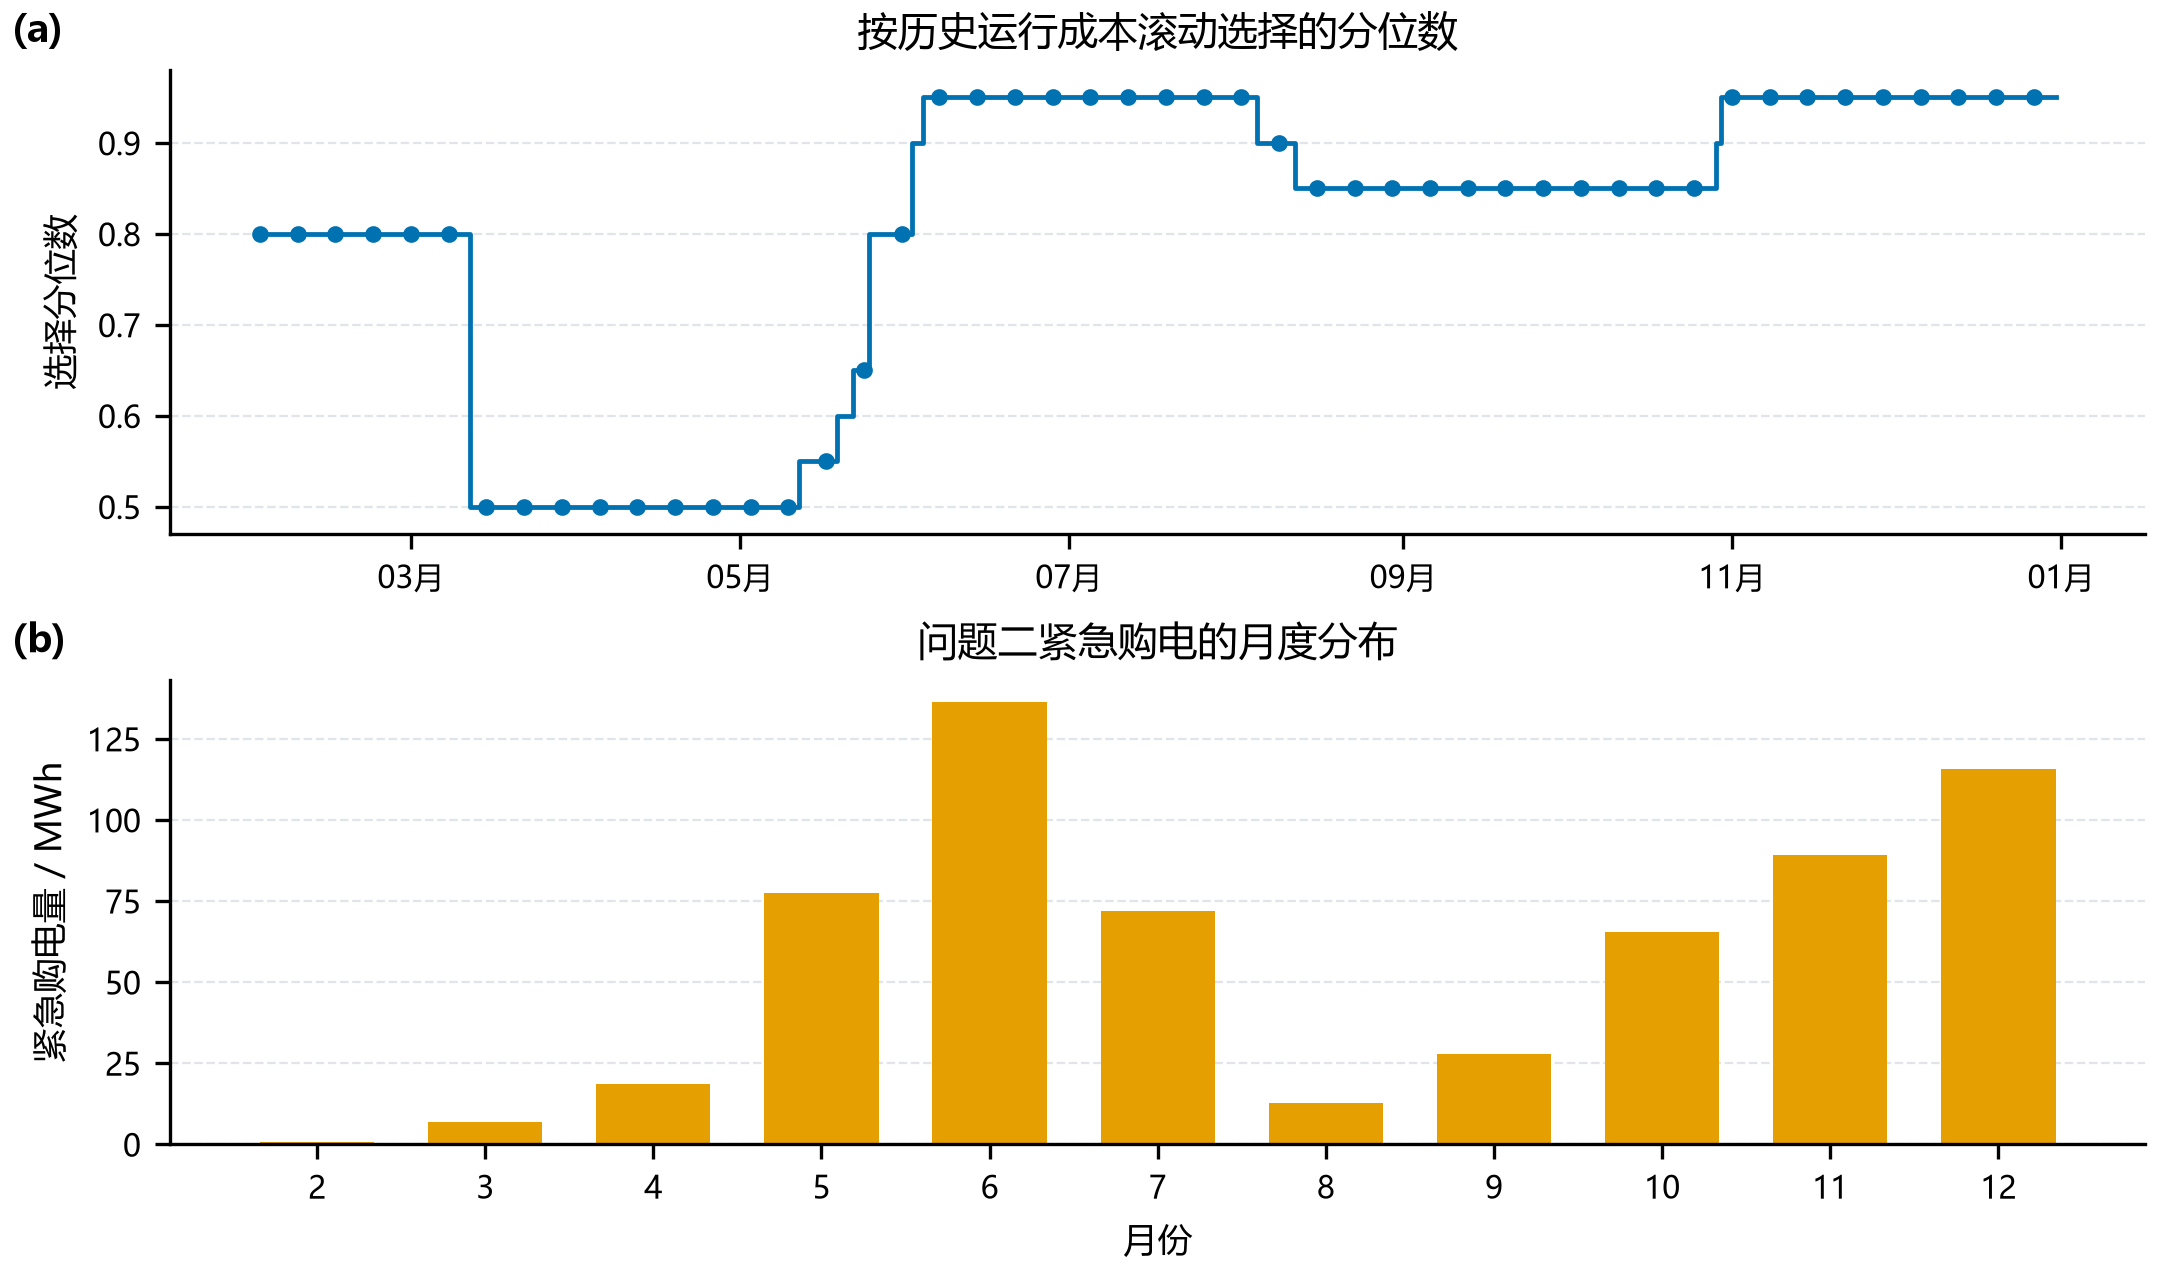
\includegraphics[width=0.93\textwidth]{图11_动态分位数与应急购电月度分布.png}
    \caption{动态分位数与应急购电月度分布}
    \label{fig:q2-alpha-emergency}
\end{figure}

\subsection{预测有效性与适用边界}

严格时间顺序的五折回测结果见表\ref{tab:forecast-validation}和图\ref{fig:forecast-validation}。问题二净负荷预测的五折平均RMSE为117.4102 kWh，高于周滞后基线79.9083 kWh，相对改善为$-48.78\%$。这不否定按运行成本选择分位数的逻辑：RMSE惩罚正负误差对称，而式\ref{eq:q2-total-cost}对正向缺口施加5倍电价，对过量计划则承担计划费，两者损失函数不同。本文因此不声称预测器在点预测精度上优于基线，只说明它把风险水平直接对齐到经济目标。

\begin{table}[htbp]
\centering
\scriptsize
\setlength{\tabcolsep}{3.5pt}
\caption{五折时间顺序样本外预测检验}\label{tab:forecast-validation}
\begin{tabular}{lrrrr}
\toprule
预测对象 & 本文RMSE & 基线RMSE & 相对改善 & 本文MAE\\
\midrule
问题二/四日前净负荷 & 117.4102 & 79.9083 & $-48.7843\%$ & 86.5700\\
问题三/四滚动负荷 & 42.1321 & 39.9246 & $-4.2738\%$ & 31.7982\\
问题三/四滚动光伏 & 28.4070 & 68.5982 & 58.0999\% & 15.1830\\
\bottomrule
\end{tabular}
\end{table}

\begin{figure}[htbp]
    \centering
    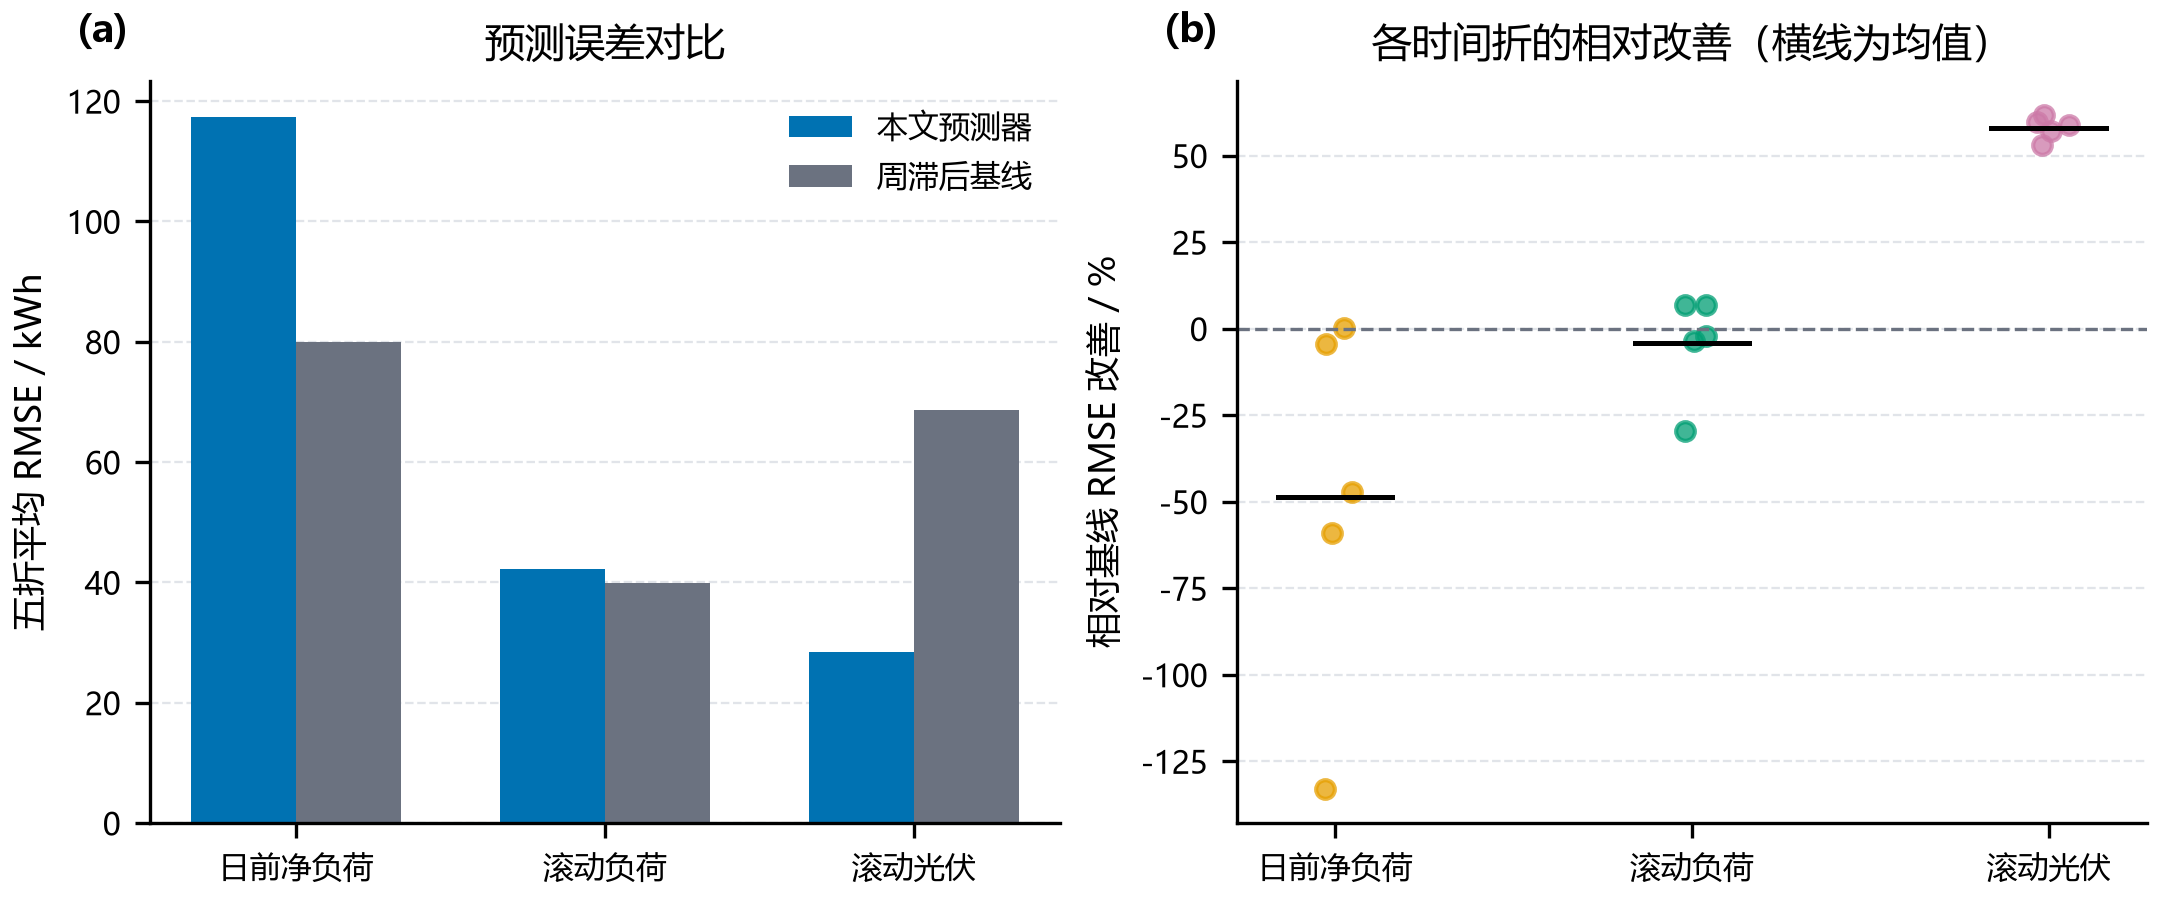
\includegraphics[width=0.92\textwidth]{图12_时间顺序样本外预测检验.png}
    \caption{时间顺序样本外预测检验}
    \label{fig:forecast-validation}
\end{figure}

问题二适用于“每日0时一次性制定计划、当日电价已知、实际偏差只由紧急购电和剩余电量结算”的机制。冻结动作的$\pm10\%$扰动属于压力情景，不等同于实际运行继续重优化；有限历史窗在极端天气或制度变化下仍可能失效。因而本问结论是：动态分位数可以表达非对称运行风险，但当前预测器的统计精度仍有提升空间。

\section{问题三：四时点滚动调整与信息价值}

\subsection{滚动调整的现实背景与信息集}

问题三允许在0:00、6:00、12:00和18:00获得新的光伏预测并修改尚未执行的购电计划。第$r$次更新的信息集包含：此前日期全部实际数据、当天$r$以前已观测负荷与光伏、最新正式发布的光伏预测、原始日前购电计划以及当前实际SOC；不包含$r$以后真实负荷或光伏。该信息边界保证每次调整只依赖决策时点已经获得的数据。

图\ref{fig:q3-solution-flow}给出问题三从预报预处理和四时点更新，到历史决策冻结、剩余时域重优化、分项结算和信息价值评价的总体求解流程。

2016年发表于《电力系统自动化》的研究基于模型预测控制建立微电网多时间尺度协调优化调度方法，为日前计划与日内滚动决策的衔接提供了依据\cite{xiao2016mpc}。

\begin{figure}[H]
    \centering
    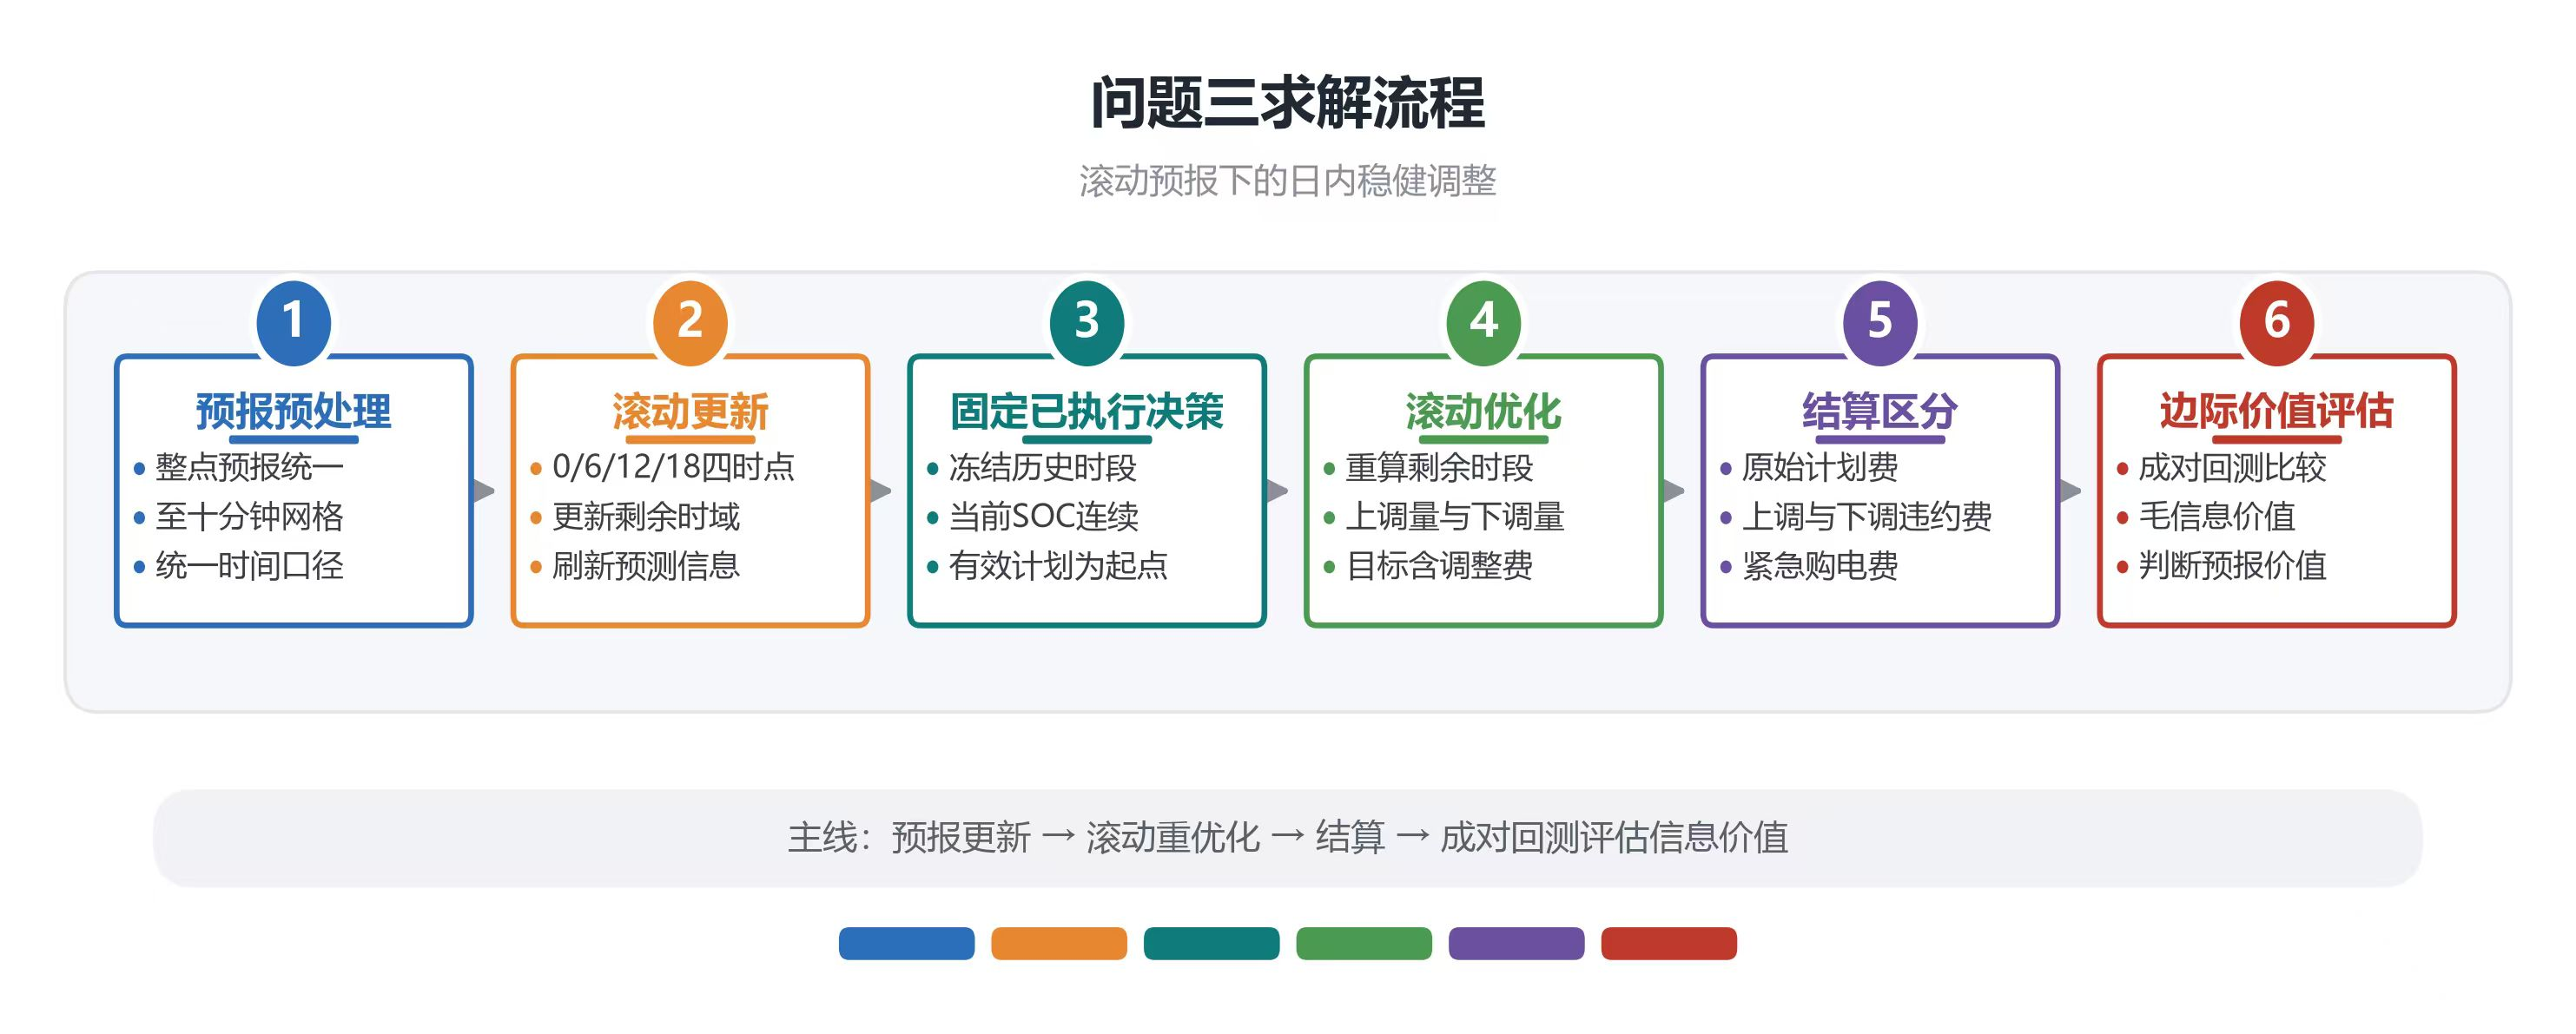
\includegraphics[width=0.98\textwidth]{图13_问题三求解流程图.jpg}
    \caption{问题三求解流程图}
    \label{fig:q3-solution-flow}
\end{figure}

\subsection{负荷与光伏预测更新}

0:00负荷预测取过去56天中同星期历史曲线的中位数，样本不足时使用全部过去日期。6、12、18时更新时，以最近12个已执行十分钟时段的实际负荷偏差修正未来预测，偏差按36个时段的时间尺度指数衰减。光伏预测取附件3最近一次正式发布的24个整点值，线性插值到十分钟网格；若更新发生在发布时间之后，则用当前已观测误差作因果校正，并按24个时段的尺度衰减。上述规则只修正未来区间，已执行历史不重新估计。

\subsection{冻结机制、SOC继承与调整结算}

令$\mathcal F_r$为$r$时刻以前已执行时段集合，滚动模型施加
\begin{equation}
(g_{d,t},c_{d,t},b_{d,t},s_{d,t})=(g^{\mathrm{exe}}_{d,t},c^{\mathrm{exe}}_{d,t},b^{\mathrm{exe}}_{d,t},s^{\mathrm{exe}}_{d,t}),
\quad t\in\mathcal F_r,
\label{eq:q3-freeze}
\end{equation}
并以最近已执行时段的$s^{\mathrm{exe}}$作为剩余时域初值。由此，每个更新节点都沿用已经实现的SOC，只冻结历史动作并重算尚未执行区间；图\ref{fig:q3-rolling-mechanism}直观展示四个执行区间以及“预测更新—重优化—执行—状态回写”的循环关系。

\begin{figure}[H]
    \centering
    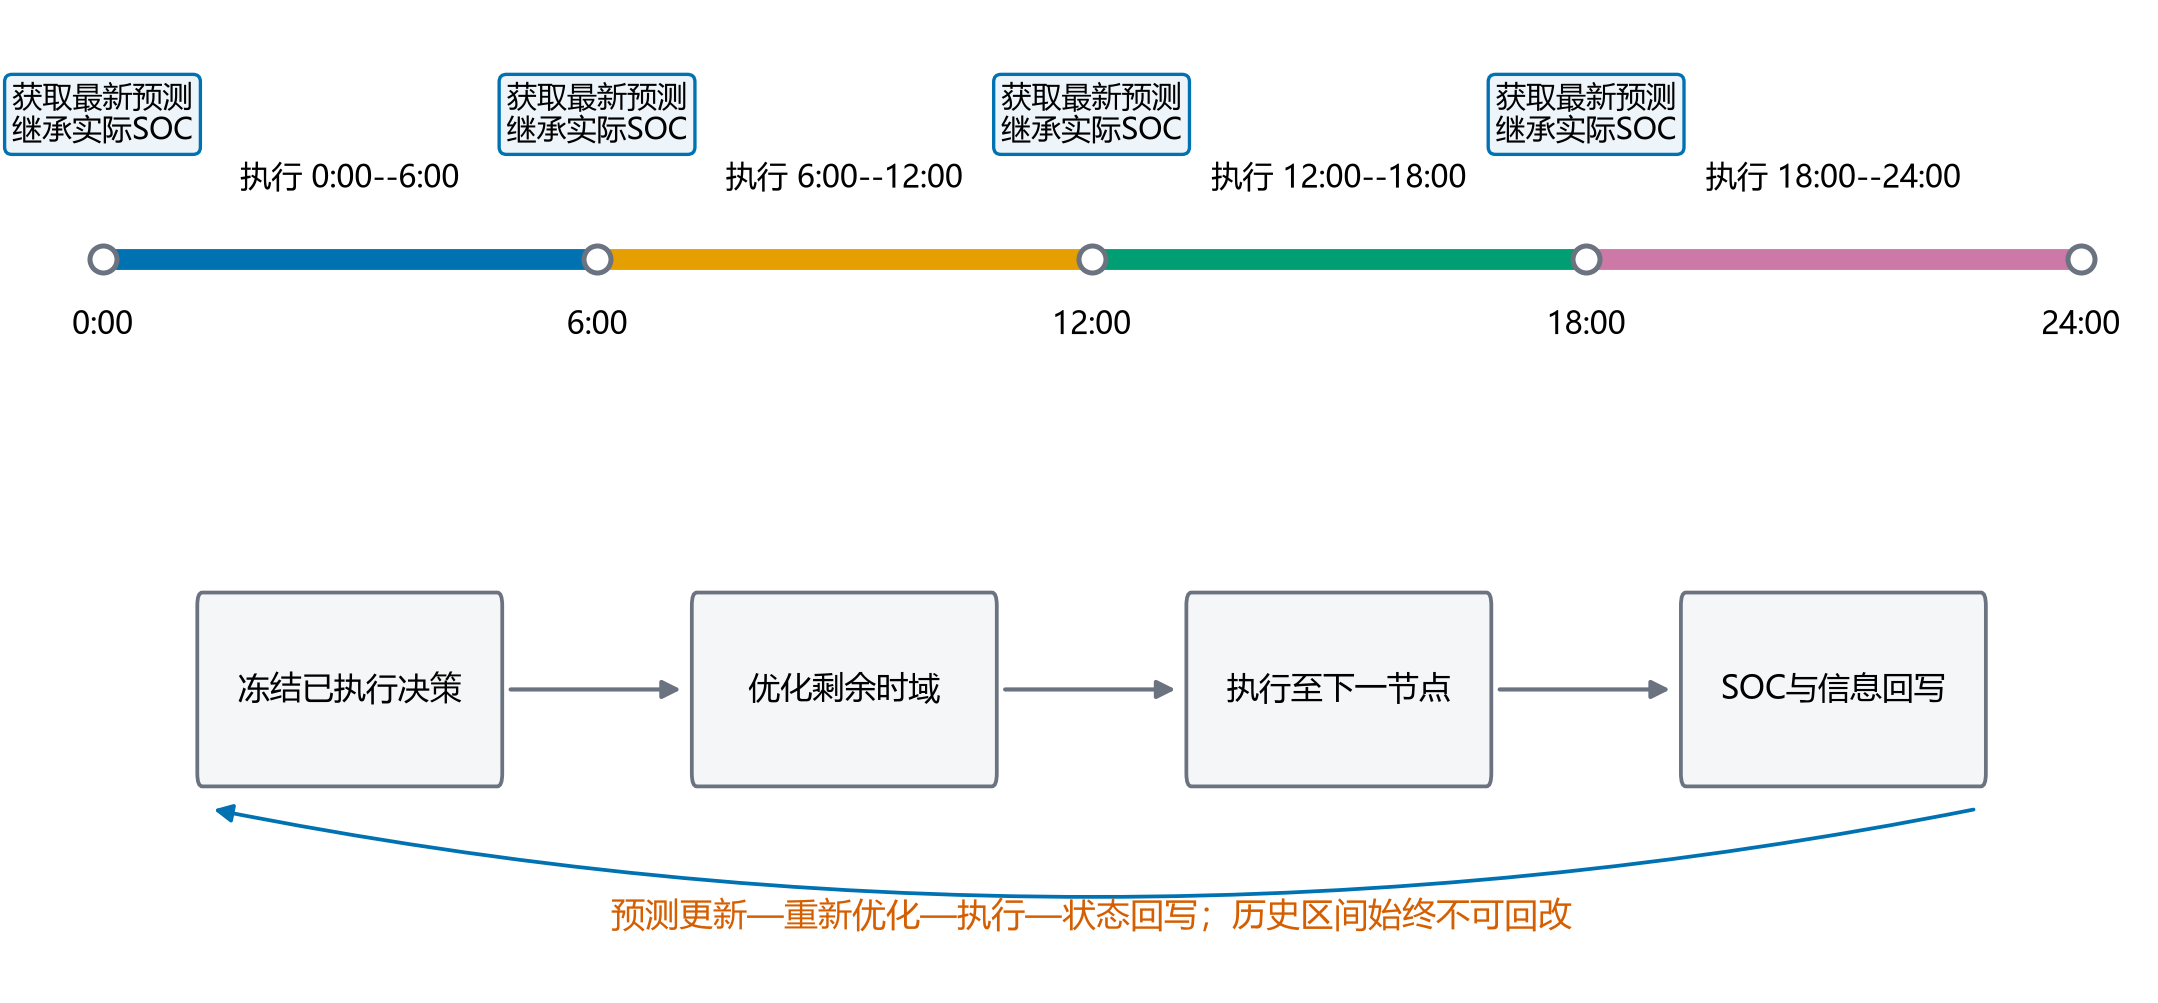
\includegraphics[width=0.96\textwidth]{图14_四时点滚动优化的信息更新机制.png}
    \caption{四时点滚动优化的执行区间与状态回写机制}
    \label{fig:q3-rolling-mechanism}
\end{figure}

对$t\notin\mathcal F_r$定义
\begin{equation}
g_{d,t}=g^0_{d,t}+u_{d,t}-v_{d,t},\qquad u_{d,t},v_{d,t}\ge0.
\label{eq:q3-adjustment}
\end{equation}
第一层滚动目标是最小化尚未执行区间的净调整费用
\begin{equation}
\min\sum_{t\notin\mathcal F_r}\pi_t\left(1.5u_{d,t}-0.5v_{d,t}\right),
\label{eq:q3-primary}
\end{equation}
再在式\ref{eq:q3-primary}最优费用容差内最小化充放电吞吐量。计划购电费在0:00已经确定，正式结算为
\begin{equation}
C^{\mathrm{tot}}_3=\sum_{d,t}\left[\pi_tg^0_{d,t}+\pi_t(1.5u_{d,t}-0.5v_{d,t})+5\pi_t e_{d,t}\right].
\label{eq:q3-total-cost}
\end{equation}
下调项为负，表示取消部分原计划后相对基准减少的净费用；但0.5倍违约成本已经体现在退款不完全中。每次MILP仍含充放电二元互斥、有限功率和跨日SOC连续，不是普通连续线性规划。

\subsection{“预测更新—优化—执行—回写”算法}

每天0:00先生成原计划$g^0$。在每个更新点$r$，读取实际SOC和最新预测，固定式\ref{eq:q3-freeze}所示历史，只对$r$至24:00求解；随后仅执行至下一个更新点，计算该段紧急购电和剩余电量，再把实际SOC写回。到18:00后执行最后6小时，日末状态直接传给次日。只有365日计算区间最后一个时段回到6000 kWh，非末日允许首末SOC不同，独立检查中有169个非末日发生跨日能量传递。

\subsection{滚动策略结果与成本解释}

表\ref{tab:q3-results}将问题三与问题二放在同一口径下比较。滚动策略总成本为16130891.40元，比日前策略减少282626.68元、降幅1.72\%。紧急购电量反而由622766.43 kWh增加到879414.55 kWh；但滚动方案把计划购电费降低1556881.39元，扣除434599.02元调整成本和新增的紧急购电费后，仍实现净节约。因此只比较紧急购电量会得出错误结论，必须同时核算计划、调整和补救费用。

\begin{table}[htbp]
\centering
\small
\caption{固定电价下日前与四时点滚动策略比较}\label{tab:q3-results}
\begin{tabular}{lrr}
\toprule
指标 & 问题二日前策略 & 问题三滚动策略\\
\midrule
计划购电量/kWh & 22702253.66 & 20388233.72\\
调整后购电量/kWh & 22702253.66 & 20257726.16\\
上调量/kWh & 0.00 & 659168.41\\
下调量/kWh & 0.00 & 789675.96\\
紧急购电量/kWh & 622766.43 & 879414.55\\
剩余电量/kWh & 4058140.12 & 1939309.80\\
计划购电费/元 & 13924597.96 & 12367716.57\\
调整费用/元 & 0.00 & 434599.02\\
紧急购电费/元 & 2488920.11 & 3328575.81\\
总成本/元 & 16413518.08 & 16130891.40\\
\bottomrule
\end{tabular}
\end{table}

图\ref{fig:q3-typical-day}展示9月23日的代表性过程。虚线日前计划在每个更新点后被重新塑形，上调和下调集中于预测发生明显变化的时段；SOC轨迹从上一日状态出发，而不是在6、12、18时被重置。图中历史段保持不变，直接验证了“只修改未来”的可执行性。

\begin{figure}[htbp]
    \centering
    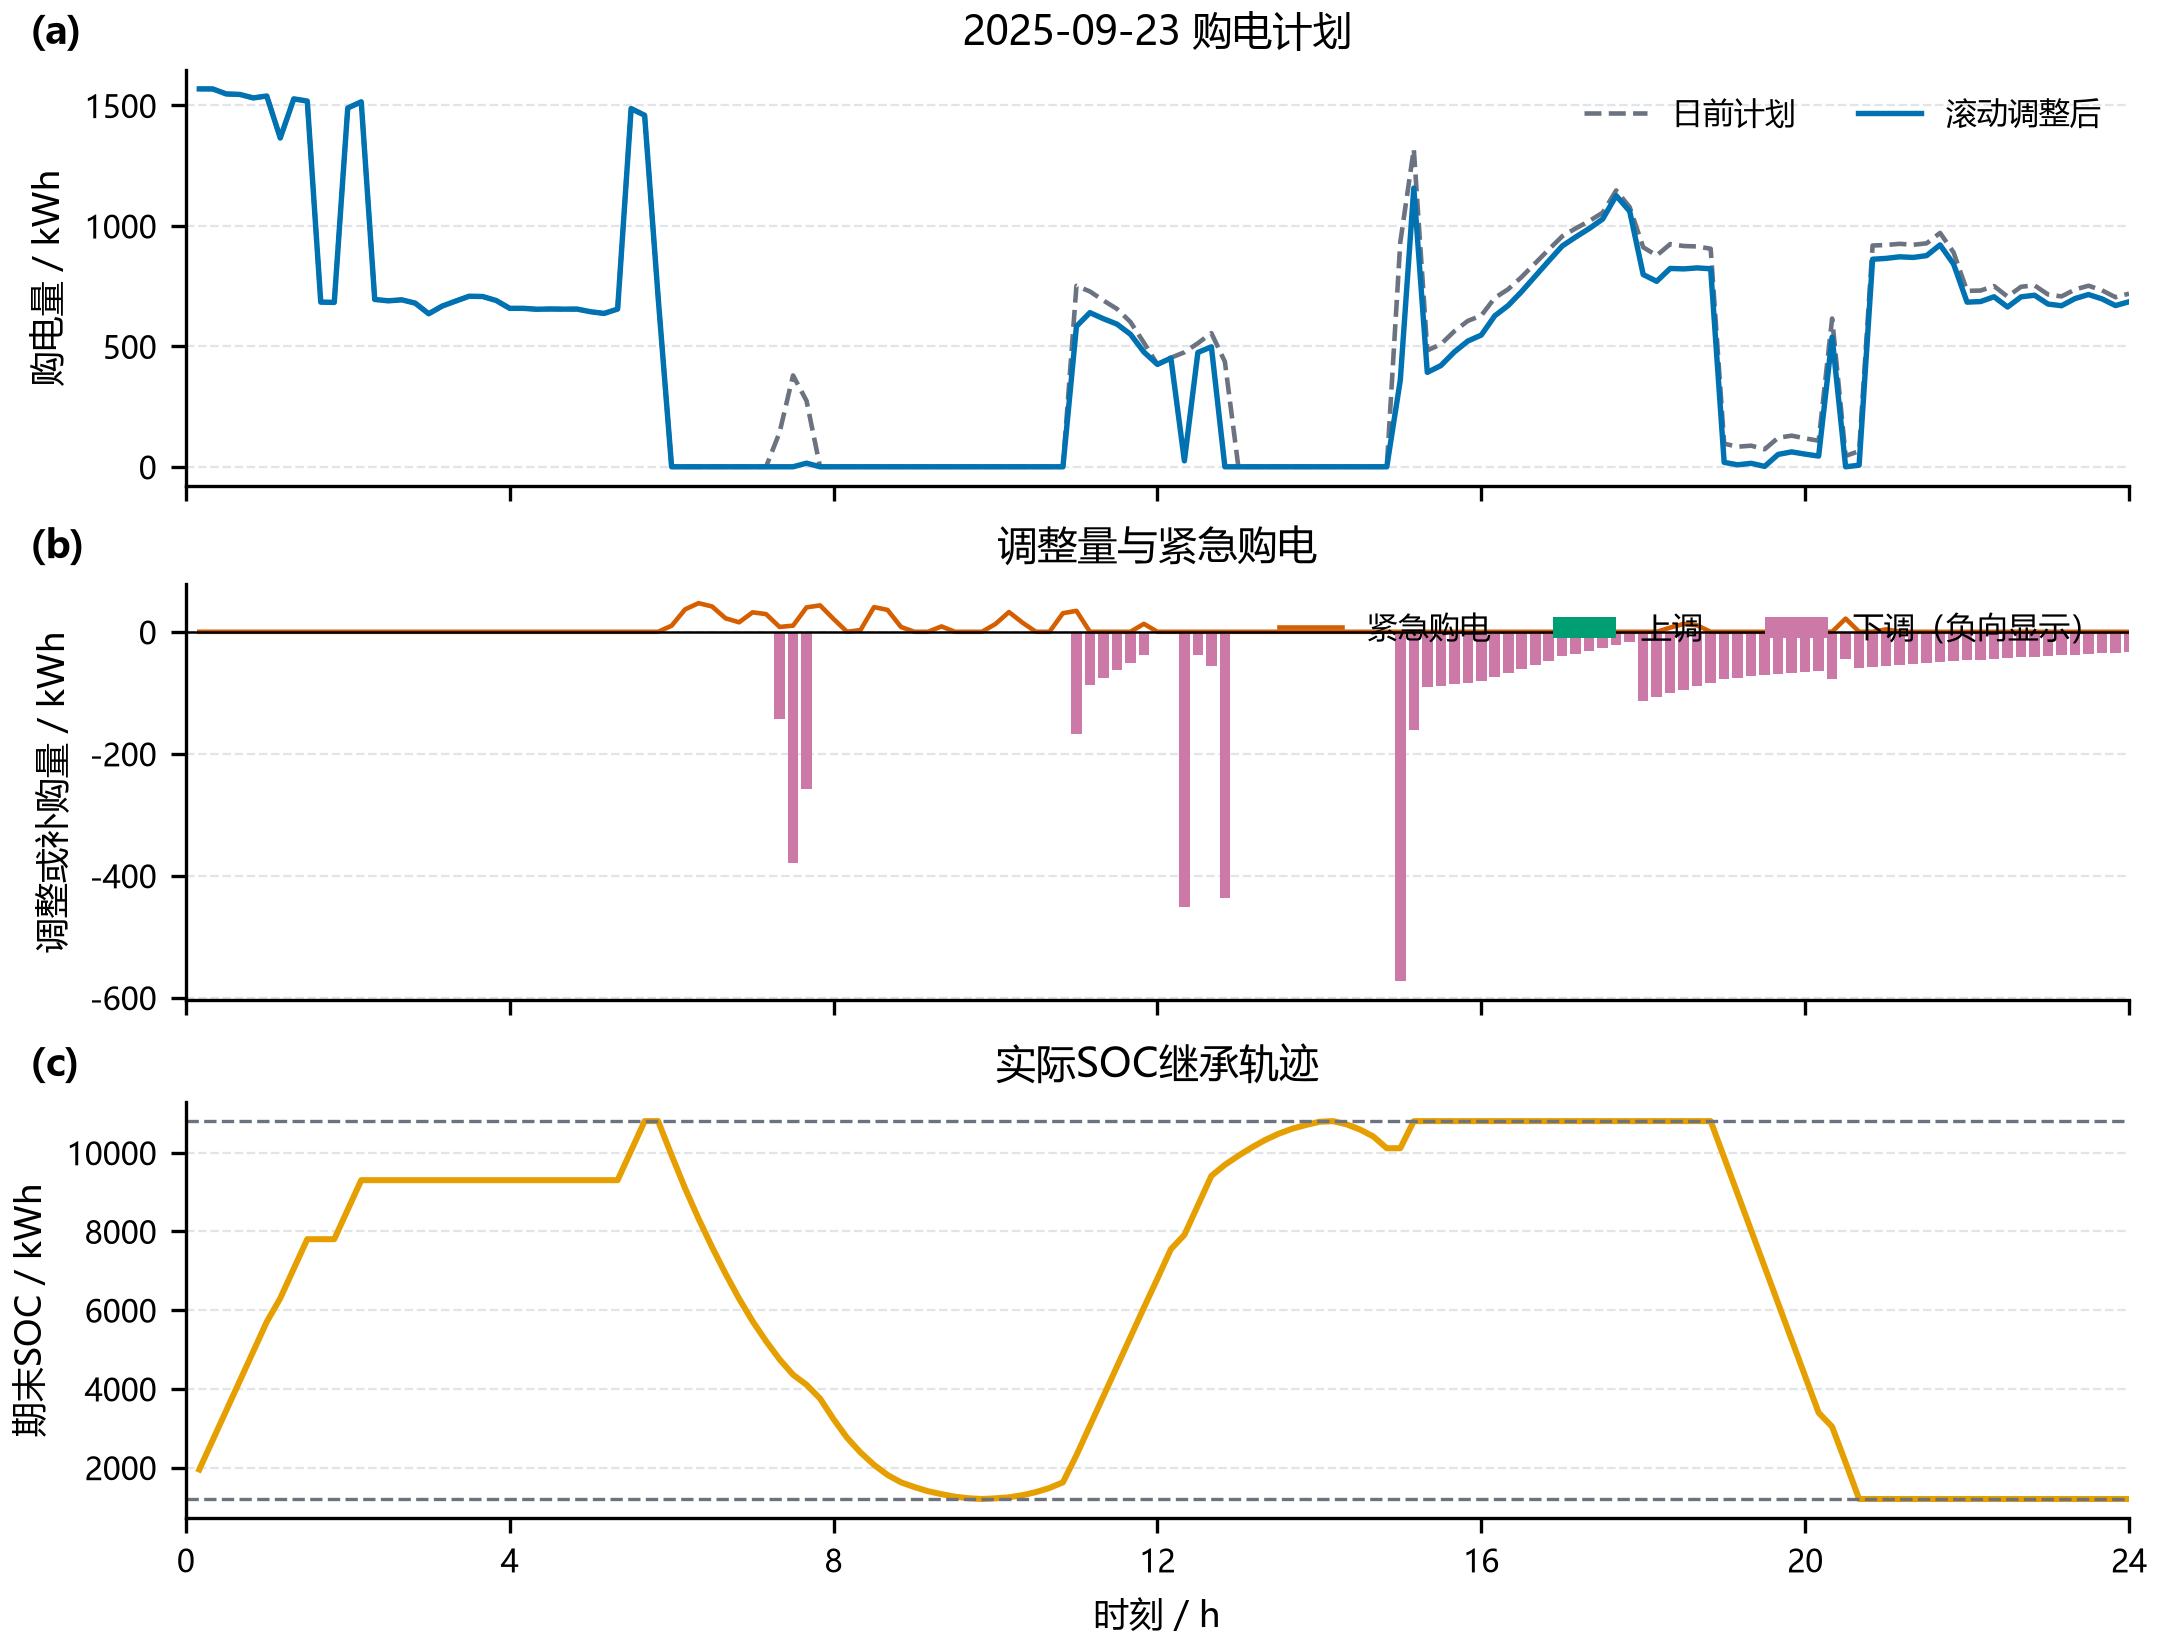
\includegraphics[width=0.91\textwidth]{图15_日前计划与四时点滚动调整的典型日对比.png}
    \caption{日前计划与四时点滚动调整的典型日对比}
    \label{fig:q3-typical-day}
\end{figure}

\subsection{四时点与八时点的信息价值}

在四时点基础上增加3、9、15、21时代理更新，定义毛信息价值为
\begin{equation}
\mathrm{VOI}_{8\mid4}=C^{\mathrm{tot}}_{4\text{点}}-C^{\mathrm{tot}}_{8\text{点}}.
\label{eq:voi}
\end{equation}
表\ref{tab:q3-voi}和图\ref{fig:q3-information-value}显示，八时点代理成本为16202052.41元，比四时点高71161.01元，故毛信息价值为负，比例为$-0.4411\%$。逐日比较中仅125天为正、209天为负。更多更新可能触发额外调整，却未必带来同等质量的增量预测；预测质量、调整费用和调度响应共同决定信息价值，更新次数本身不能保证降本。

\begin{table}[htbp]
\centering
\small
\caption{四时点与八时点代理方案的信息价值}\label{tab:q3-voi}
\begin{tabular}{lrr}
\toprule
指标 & 四时点 & 八时点代理\\
\midrule
正式评价期总成本/元 & 16130891.40 & 16202052.41\\
八时点相对四时点成本差/元 & -- & 71161.01\\
毛信息价值/元 & \multicolumn{2}{c}{$-71161.01$}\\
相对信息价值 & \multicolumn{2}{c}{$-0.4411\%$}\\
逐日正/负信息价值天数 & \multicolumn{2}{c}{125/209}\\
\bottomrule
\end{tabular}
\end{table}

\begin{figure}[htbp]
    \centering
    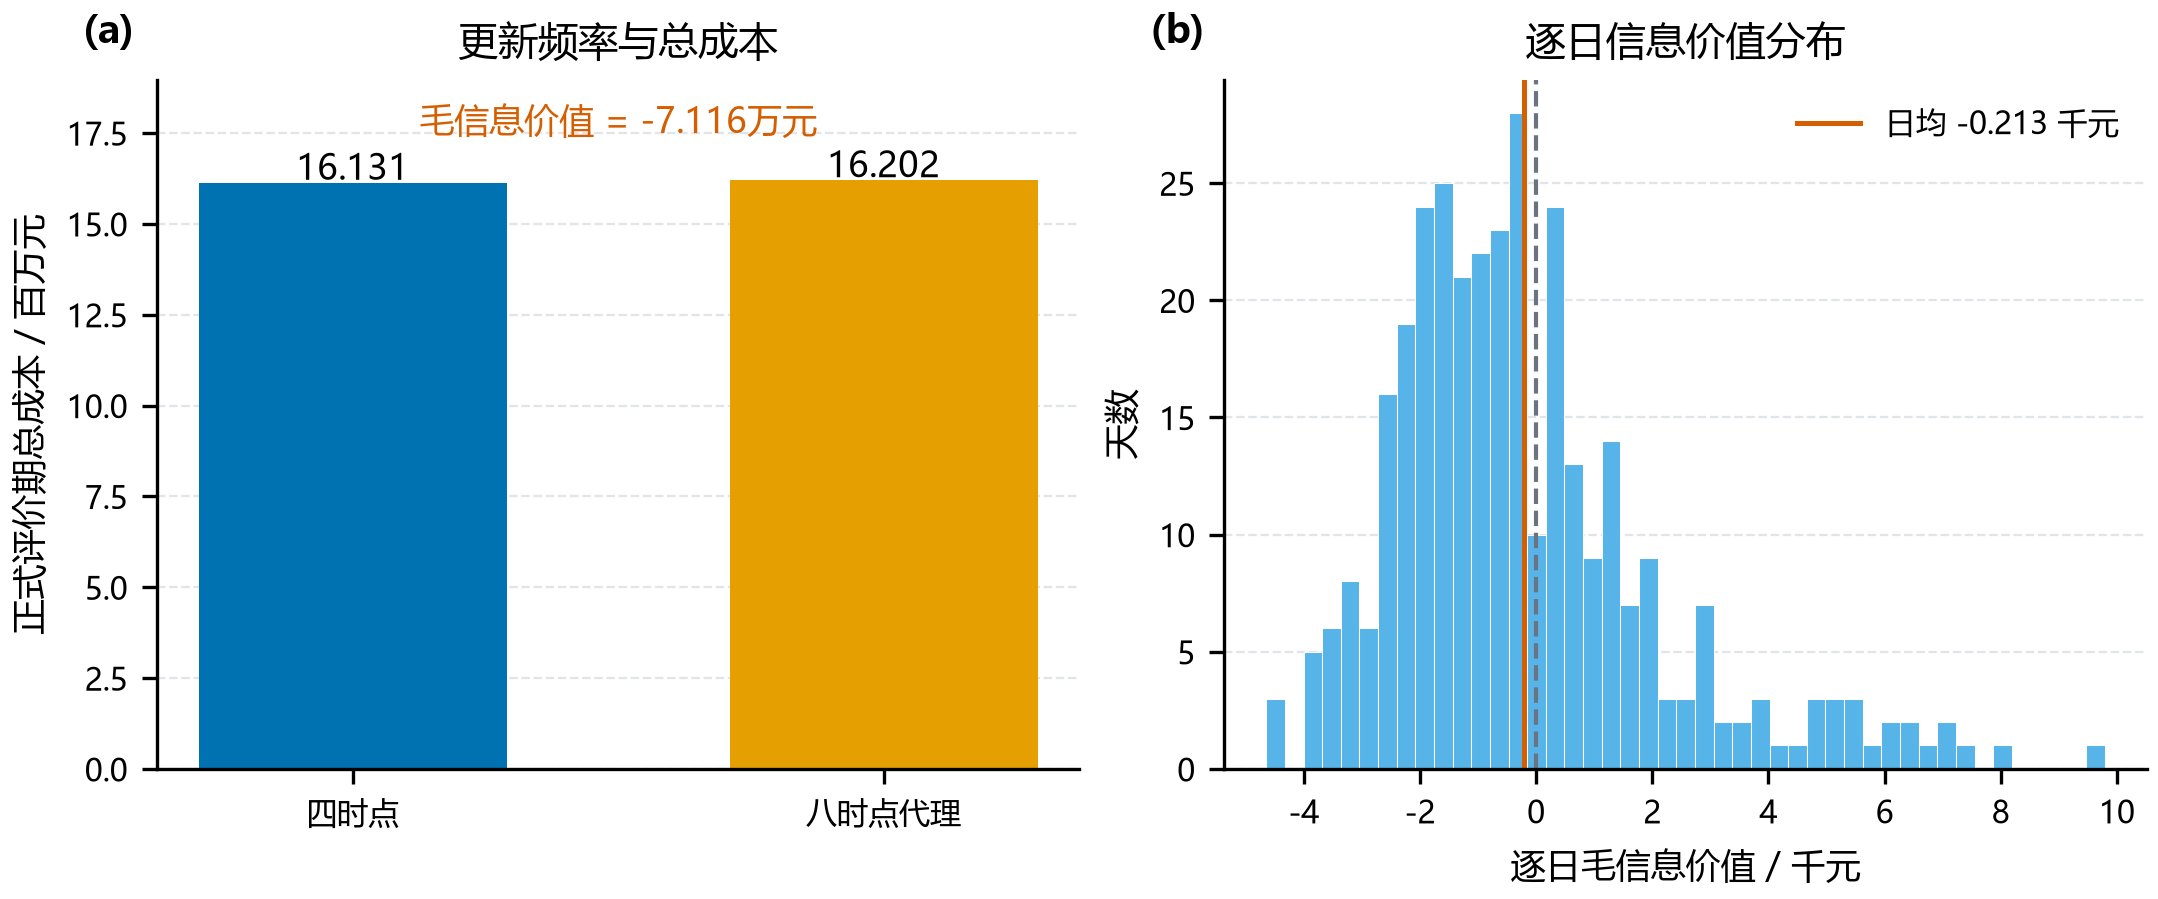
\includegraphics[width=0.91\textwidth]{图16_不同预报更新频率下的信息价值比较.png}
    \caption{不同预报更新频率下的信息价值比较}
    \label{fig:q3-information-value}
\end{figure}

\subsection{本问小结}

四时点滚动策略通过压缩高成本的过量计划电量，在紧急购电增加的情况下仍降低总成本1.72\%。节点可行性检查表明已执行动作未被回改、SOC逐段继承、跨日衔接残差为0。八时点方案则没有产生正经济价值，因此现阶段更合理的建议是改进新增时点预测质量和调整规则，再决定是否提高发布频率。

\section{问题四：波动电价下的日前与滚动策略}

\subsection{波动电价特征与可见性假设}

问题四把附件4的逐十分钟价格引入同一物理模型。正式评价期波动电价均值0.7575元/kWh，略低于固定价均值0.7662元/kWh，但标准差由0.3133增至0.3361，范围扩展到0.0076--1.7936元/kWh。图\ref{fig:q4-price-comparison}显示，均值接近并不意味着成本接近：更宽的尾部和每天不同的价格路径会改变储能何时充放电。

图\ref{fig:q4-solution-flow}概括问题四接入波动电价后，分别求解日前计划与滚动调整策略，并在统一约束和结算口径下进行成本、应急购电及稳定性比较的过程。

\begin{figure}[H]
    \centering
    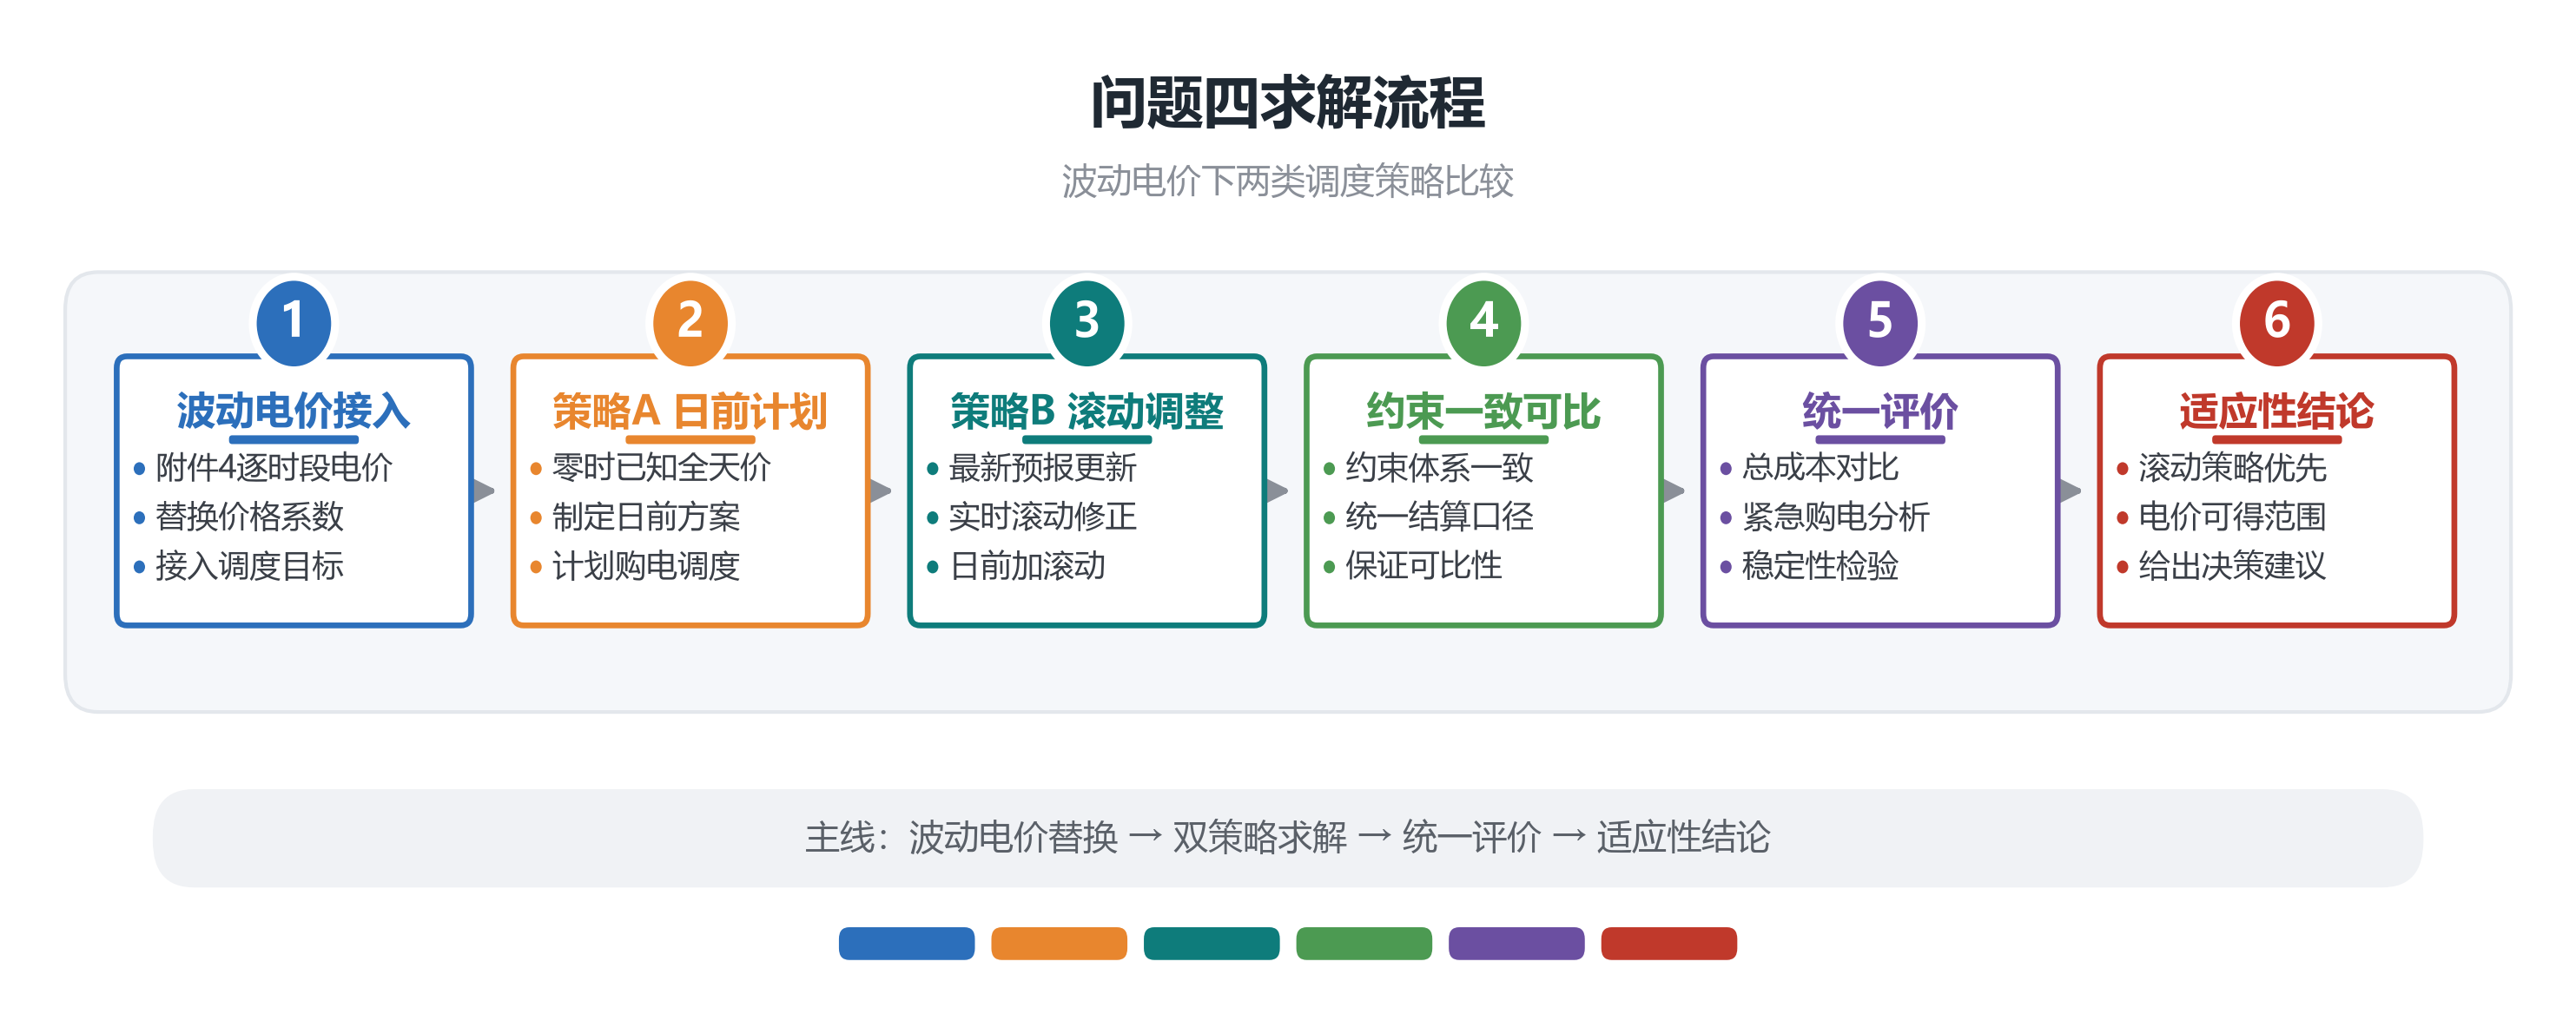
\includegraphics[width=0.98\textwidth]{图17_问题四求解流程图.png}
    \caption{问题四求解流程图}
    \label{fig:q4-solution-flow}
\end{figure}

\begin{figure}[htbp]
    \centering
    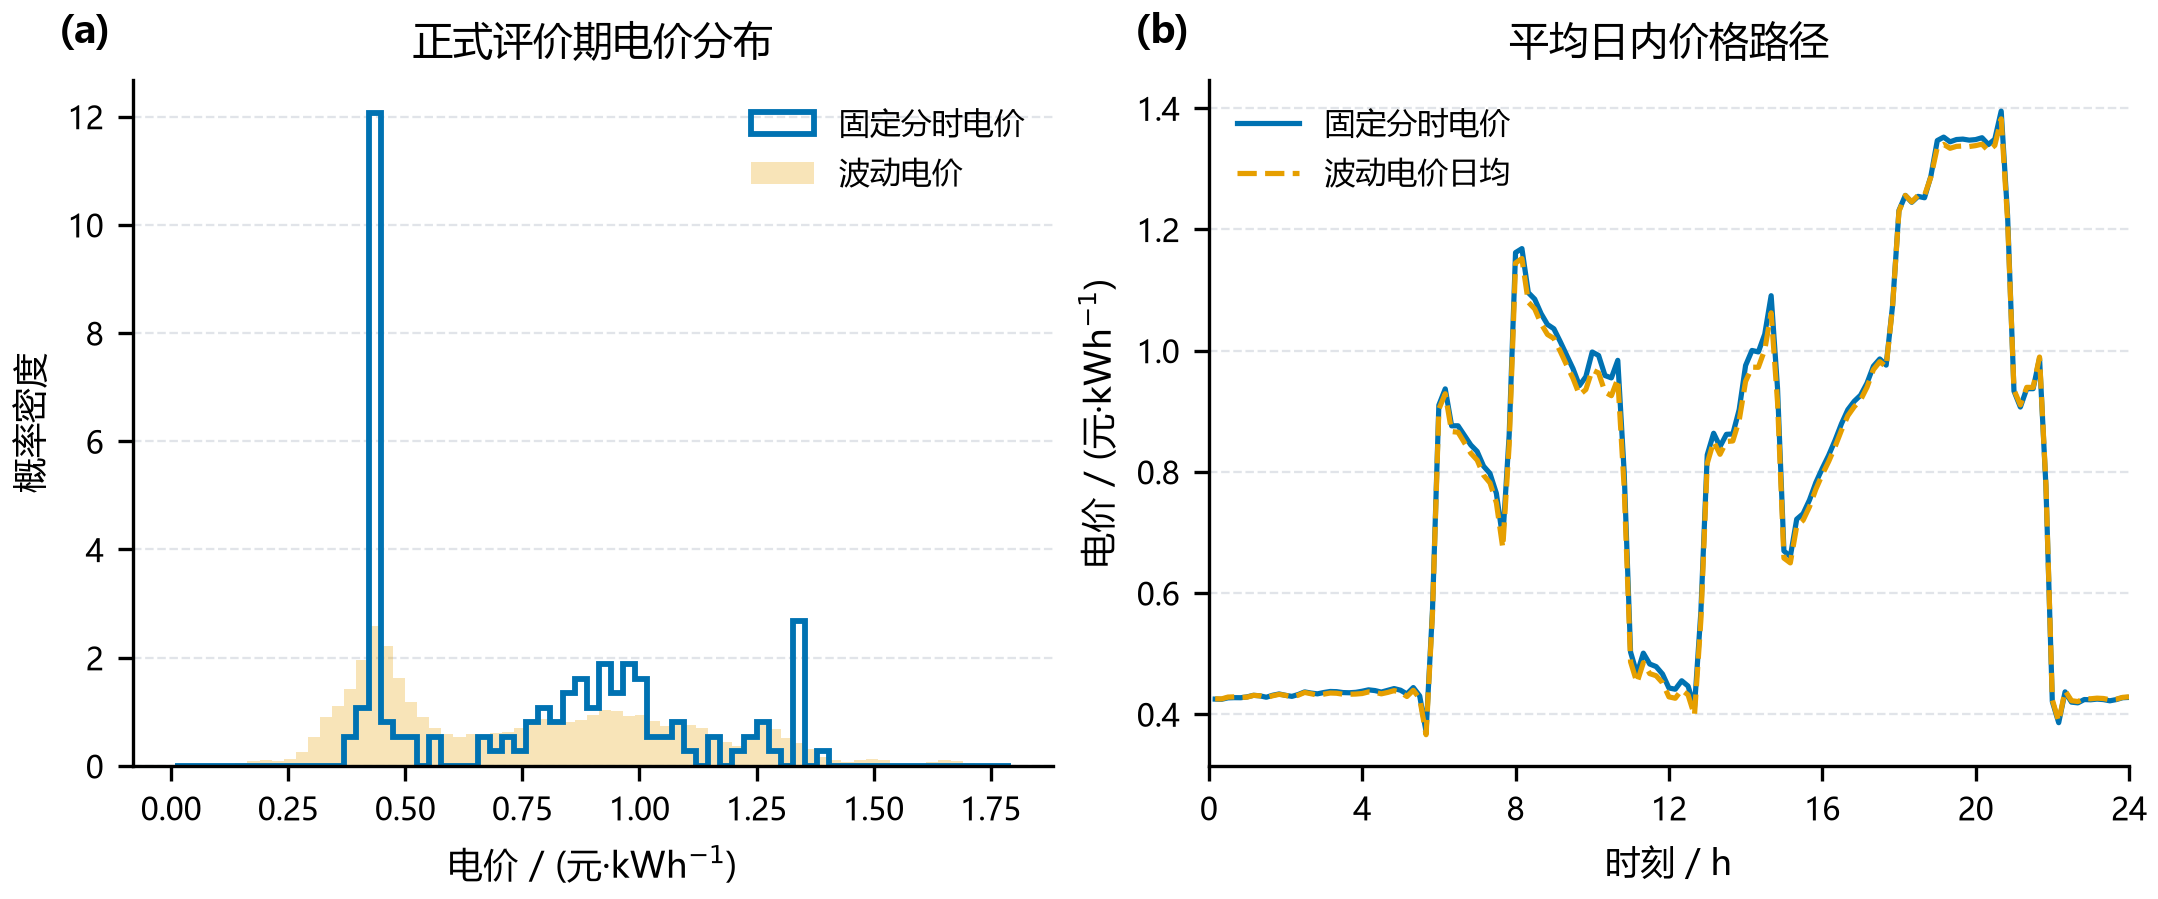
\includegraphics[width=0.93\textwidth]{图18_固定电价与波动电价分布对比.png}
    \caption{固定电价与波动电价分布对比}
    \label{fig:q4-price-comparison}
\end{figure}

当前正式实现假定当日电价路径在0:00已经可用，因此日前策略可使用当天完整附件4价格，滚动策略也在各更新点使用同一已知价格路径。该假设决定了问题四是“已知波动价格下的调度响应”而非“价格预测问题”；若实际市场只逐时发布价格，则必须增加严格因果的电价预测器并重新回测，不能直接沿用本文数值结论。

\subsection{统一物理层下的两类策略}

问题四日前分支完全继承问题二：采用动态配对净负荷分位数，求解含二元互斥的两阶段MILP，实际偏差按5倍当时电价紧急购电。滚动分支完全继承问题三：0、6、12、18时冻结历史、继承实际SOC、重新优化剩余时域，并按式\ref{eq:q3-total-cost}结算上下调与紧急购电。两类策略只改变价格序列，不改变容量、功率、效率、互斥和跨日SOC口径，因而成本差异可归因于价格与信息更新的共同作用。

\subsection{总体成本与购电构成}

表\ref{tab:q4-results}给出波动电价结果。日前策略总成本17148794.62元，滚动策略16864403.38元，节约284391.24元、降幅1.6584\%。滚动策略把计划购电量减少231.46万kWh，并把剩余电量从405.94万kWh降至193.20万kWh；与此同时紧急购电增加25.54万kWh。与固定价情形相同，成本改善来自减少过量计划和重排储能，而非单纯追求最低紧急购电量。

\begin{table}[htbp]
\centering
\small
\caption{波动电价下日前与滚动策略结果}\label{tab:q4-results}
\begin{tabular}{lrr}
\toprule
指标 & 问题四日前策略 & 问题四滚动策略\\
\midrule
计划购电量/kWh & 22753519.79 & 20438906.42\\
调整后购电量/kWh & 22753519.79 & 20302690.07\\
上调量/kWh & 0.00 & 659811.63\\
下调量/kWh & 0.00 & 796027.98\\
紧急购电量/kWh & 624612.25 & 879985.14\\
剩余电量/kWh & 4059386.28 & 1931978.89\\
计划购电费/元 & 14461314.89 & 12883389.48\\
调整费用/元 & 0.00 & 486968.64\\
紧急购电费/元 & 2687479.73 & 3494045.26\\
总成本/元 & 17148794.62 & 16864403.38\\
\bottomrule
\end{tabular}
\end{table}

相较固定价，波动价使日前总成本增加735276.55元（4.48\%），使滚动总成本增加733511.98元（4.55\%）。尽管波动价格的算术均值略低，但高净负荷与高价在部分时段重合，且储能受功率、容量和效率限制，无法完全把所有购电移到极低价区间。因此“平均价格下降”并不能推出“运行总成本下降”。

\subsection{月度与典型日调度行为}

图\ref{fig:q4-monthly-cost}显示四种策略在6、7和12月成本共同上升，与第5节月度净负荷高位一致；滚动策略在多数月份低于对应日前策略，但不是每一天都占优。固定价滚动方案逐日成本较日前方案降低198天、升高136天；波动价下分别为195天和139天，说明全年节约由大量大小不一的日差额累积，而不是逐日支配。

\begin{figure}[htbp]
    \centering
    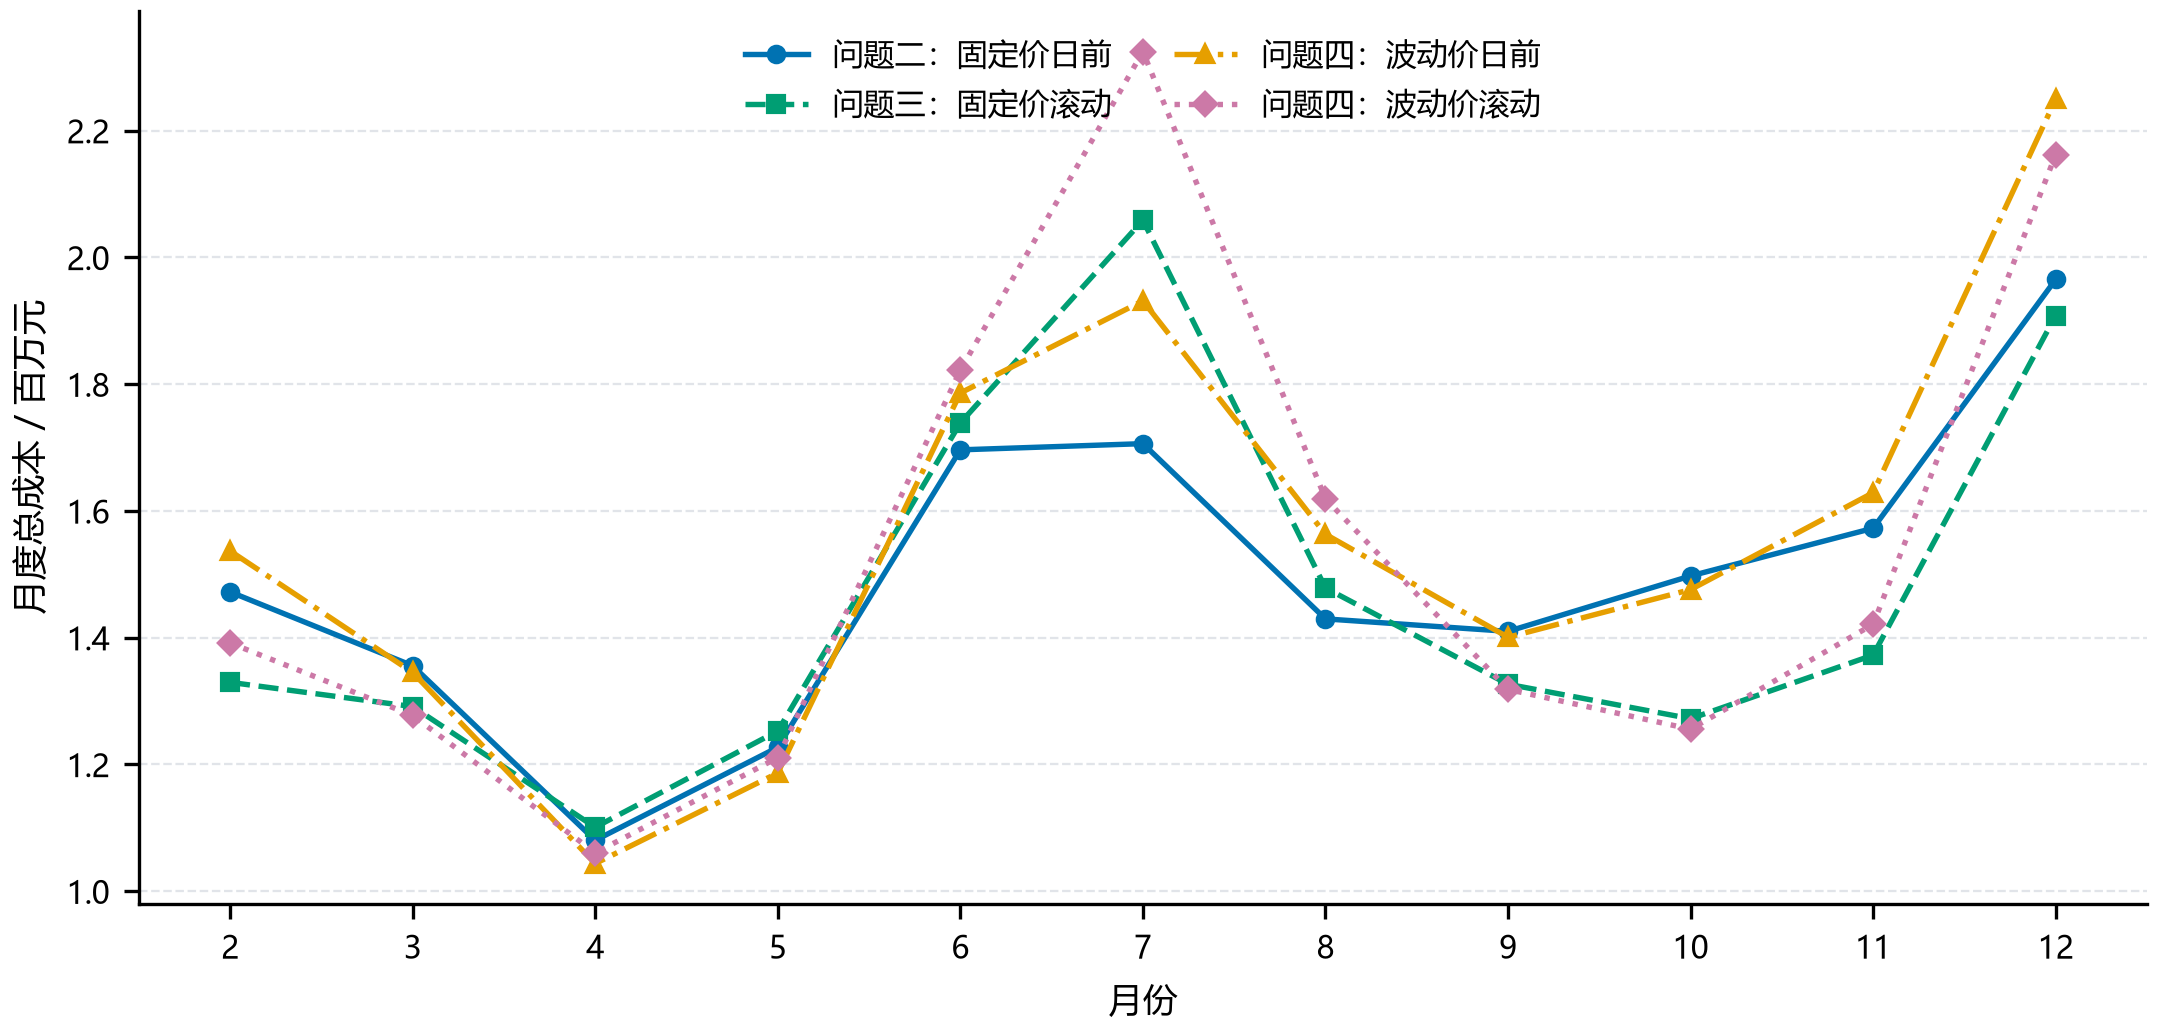
\includegraphics[width=0.92\textwidth]{图19_四种调度策略的月度成本比较.png}
    \caption{四种调度策略的月度成本比较}
    \label{fig:q4-monthly-cost}
\end{figure}

图\ref{fig:q4-typical-day}给出9月23日波动价格下的滚动调度。低价区间出现集中充电，高价且净负荷较高时段出现放电；计划与调整后购电曲线在预测更新后分离，说明收益不仅来自误差修正，也来自把有限SOC重新配置到更有价值的价格时段。

\begin{figure}[htbp]
    \centering
    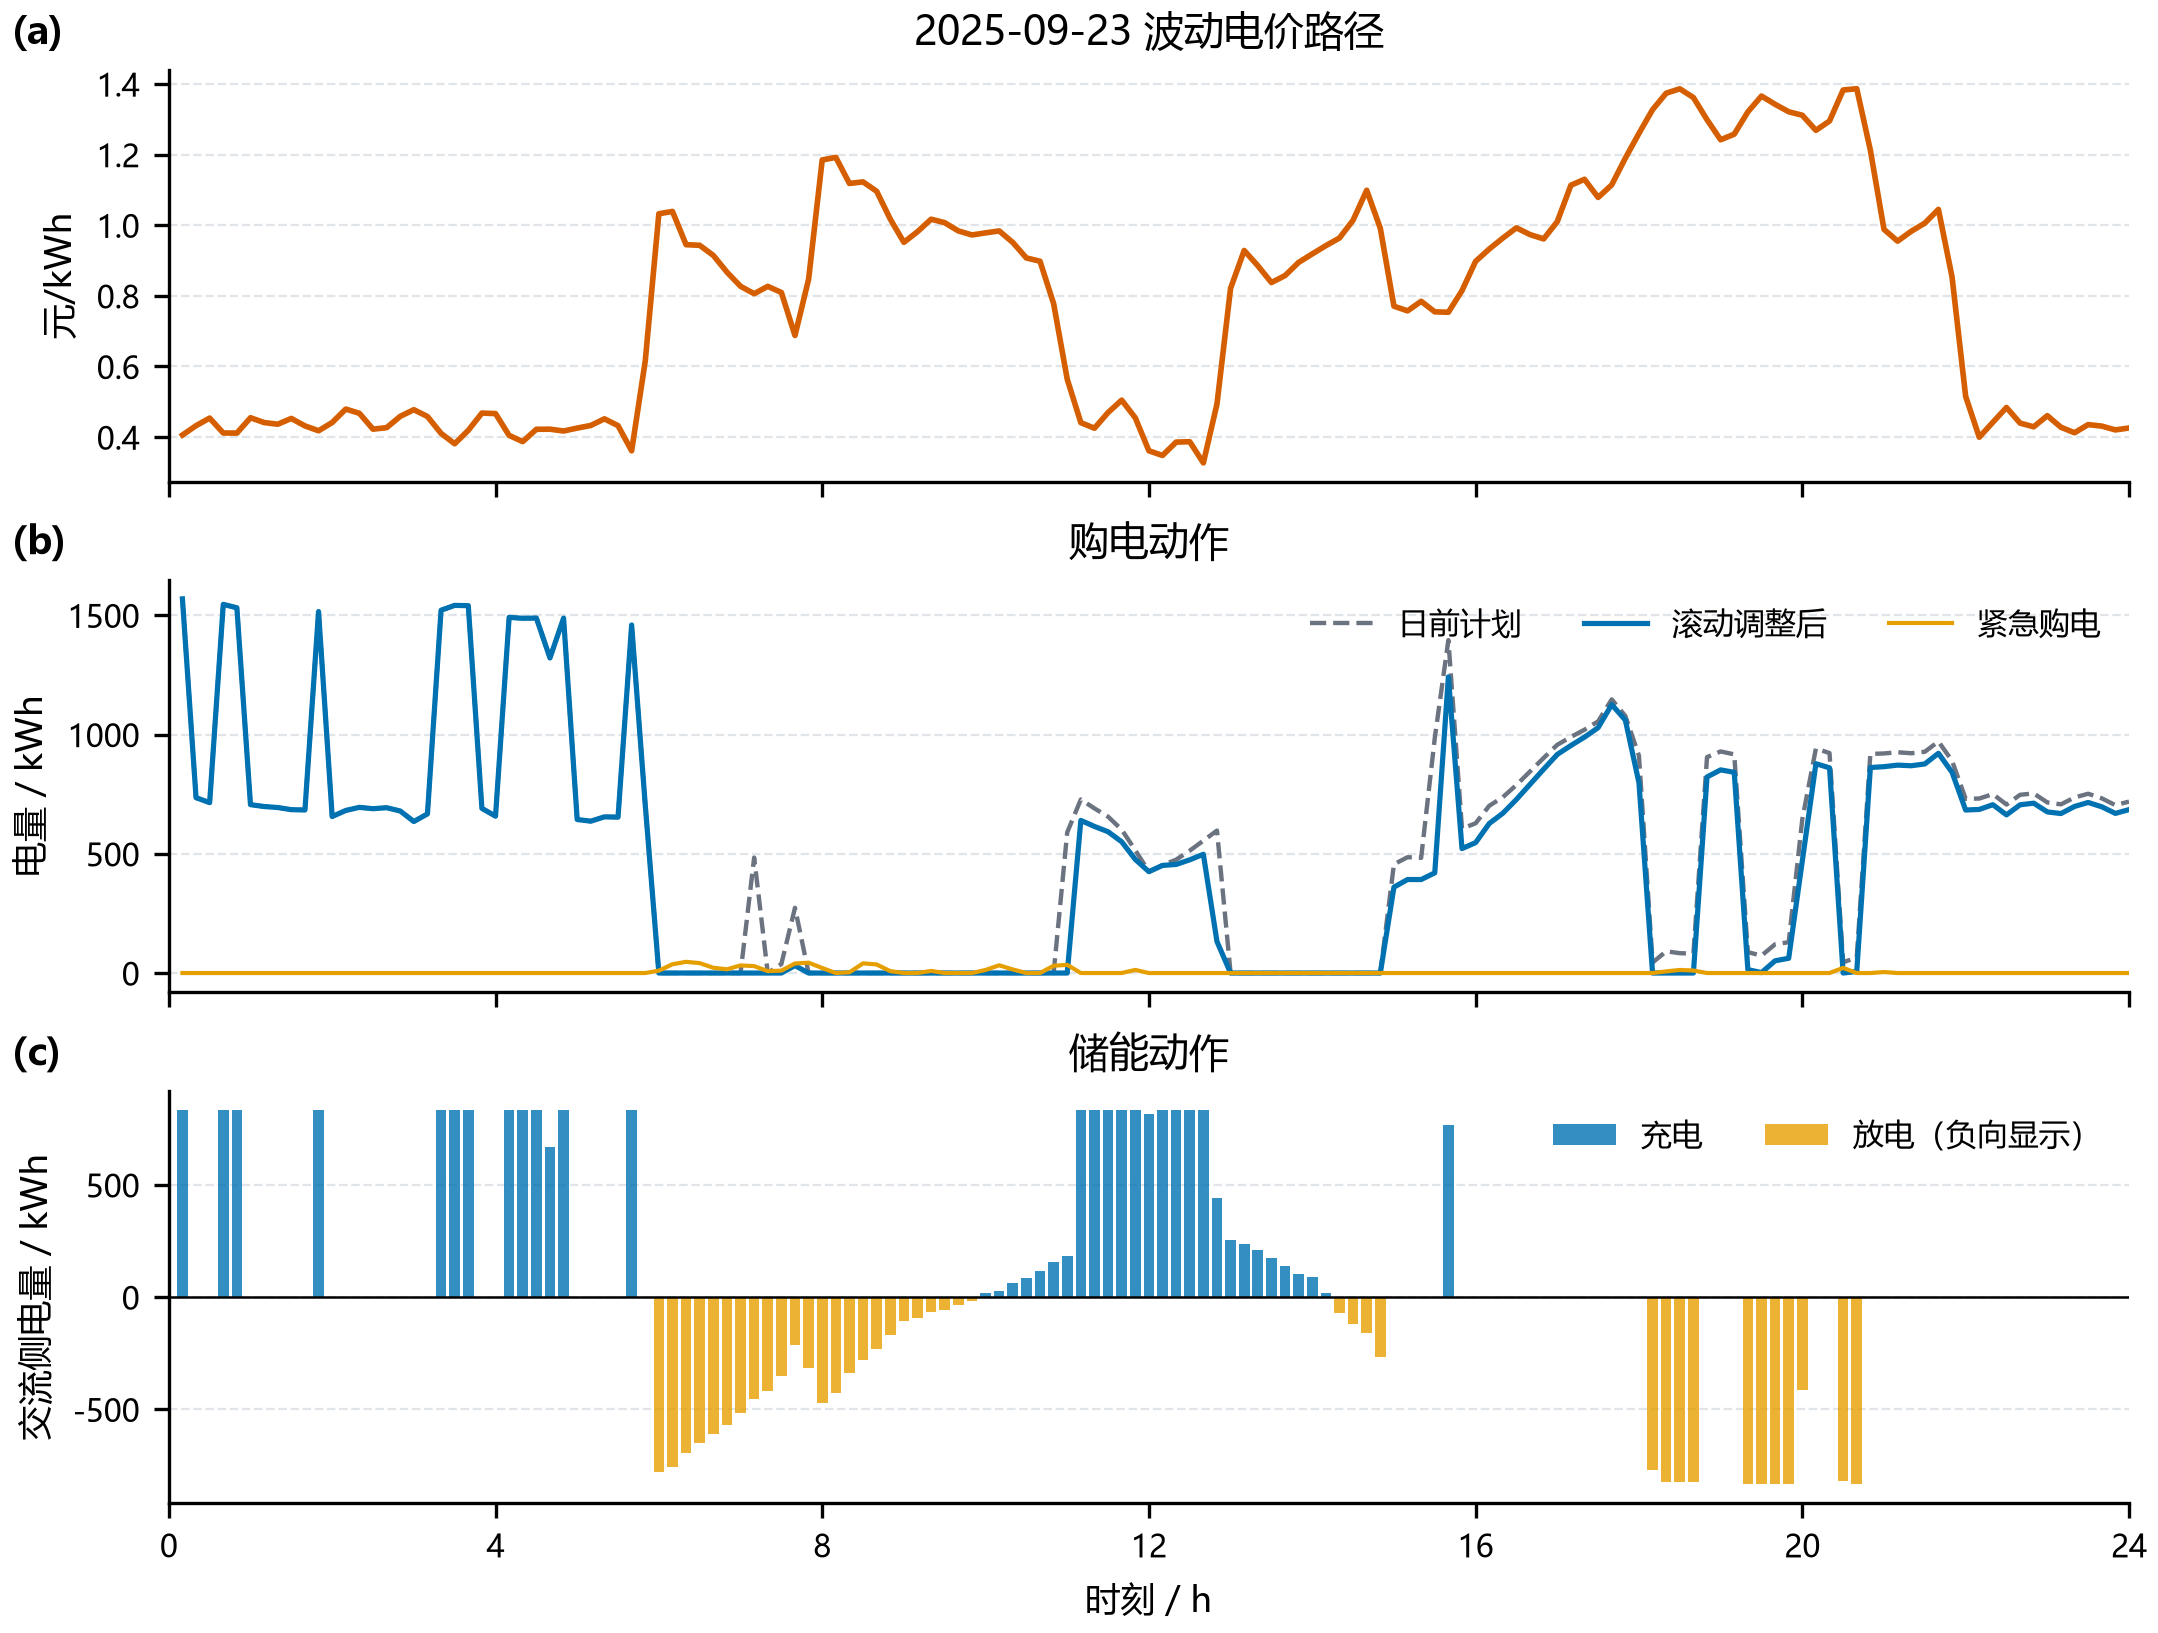
\includegraphics[width=0.91\textwidth]{图20_波动电价下滚动策略的典型日调度.png}
    \caption{波动电价下滚动策略的典型日调度}
    \label{fig:q4-typical-day}
\end{figure}

总体成本图\ref{fig:q234-total-cost}把四个正式策略放在统一坐标中。固定价四时点滚动方案成本最低，波动价日前方案最高；但该排序同时受价格序列和可用预测信息影响，不能解释为某一种算法在任意市场机制下必然占优。

\begin{figure}[htbp]
    \centering
    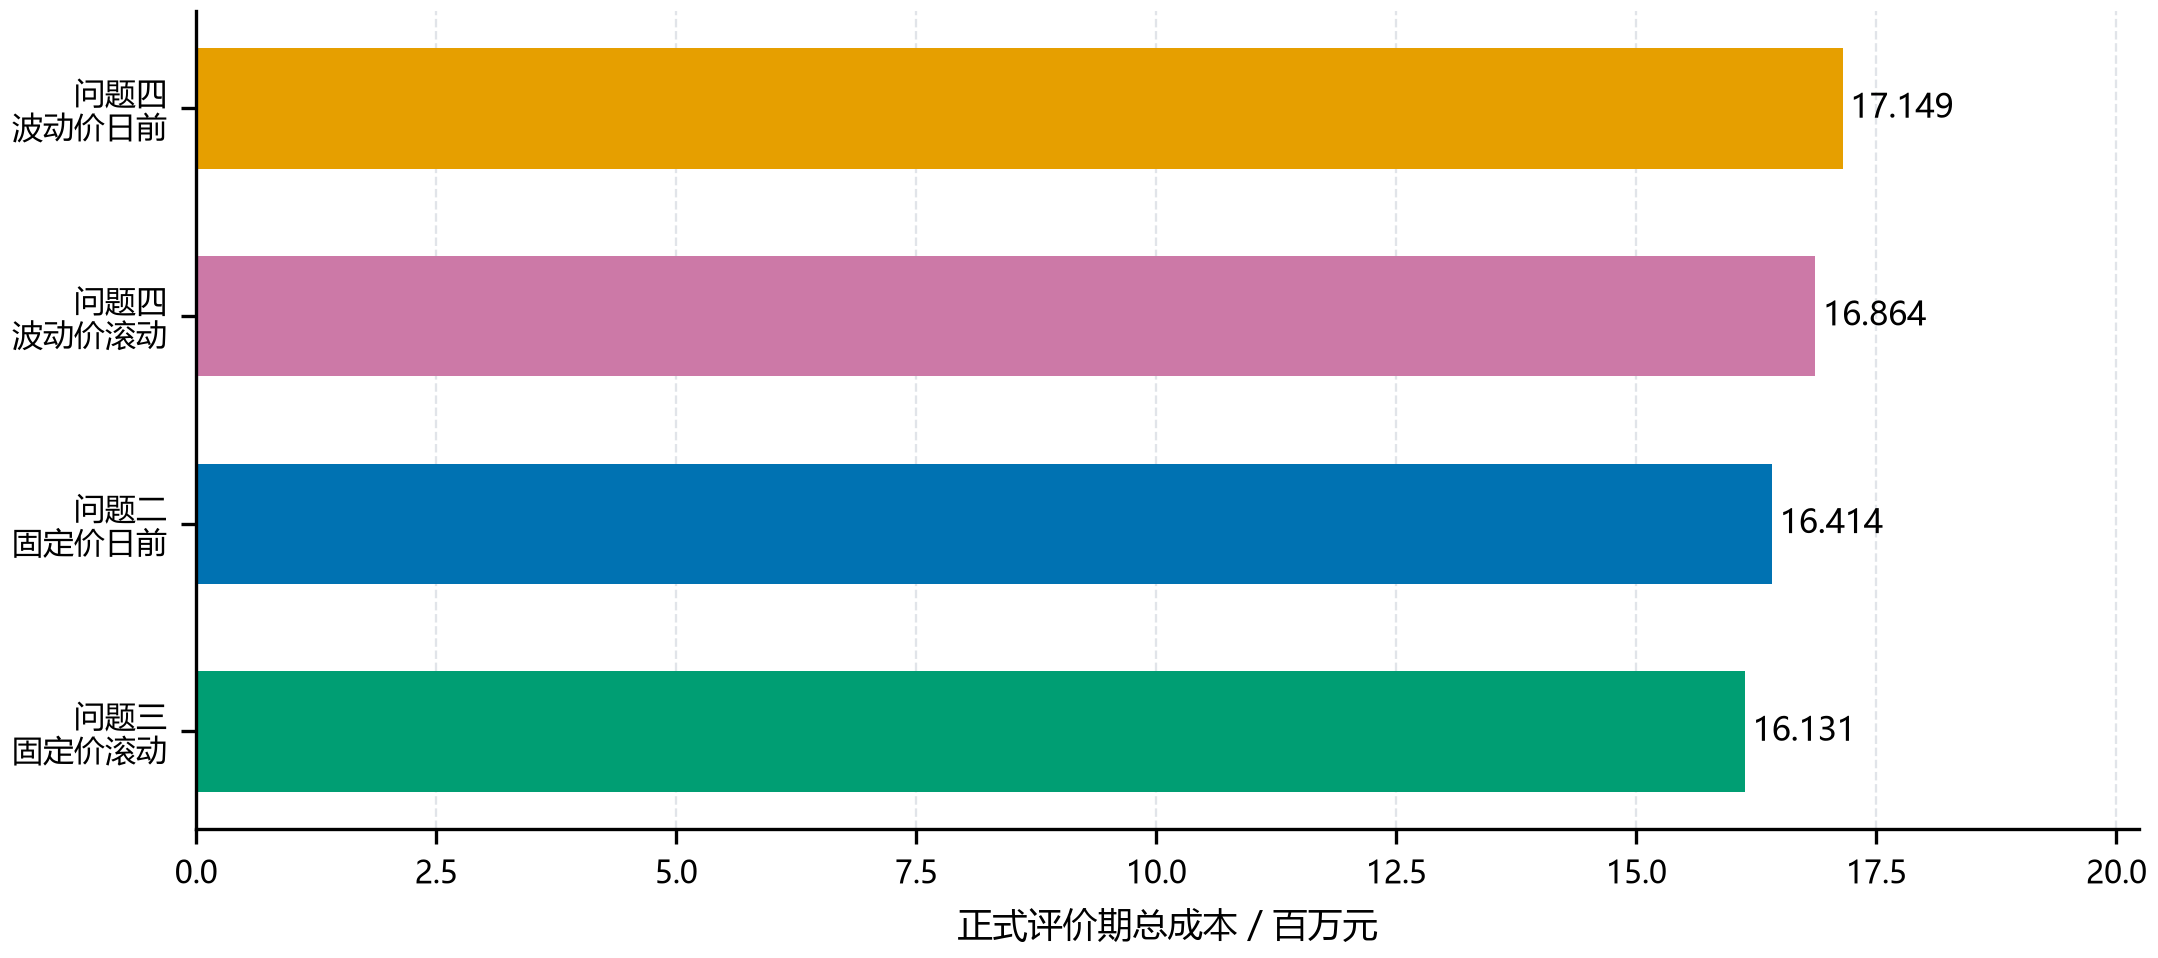
\includegraphics[width=0.88\textwidth]{图21_不同问题与调度策略的全年总成本比较.png}
    \caption{不同问题与调度策略的全年总成本比较}
    \label{fig:q234-total-cost}
\end{figure}

\subsection{本问小结与结论边界}

在“当日完整价格路径0:00可见”的假设下，波动价滚动策略较波动价日前策略降低1.66\%，但其绝对成本仍高于固定价滚动方案。波动电价收益或损失既取决于预测误差，也取决于价格与净负荷的相关位置以及储能约束。若价格发布机制改变、出现实时结算或允许售电，目标函数和可用信息集都需重新定义。

\section{模型检验与结果边界}

\subsection{数值可行性检验}

不以求解器返回成功作为唯一依据，而是对输出逐时独立回代。表\ref{tab:numerical-checks}集中列出供需平衡、SOC递推、边界、互斥、跨日衔接和成本对账，避免在四个问题中重复堆砌同一组残差。所有残差远低于$10^{-5}$ kWh容差，问题二至四的计算区间初末SOC均为6000 kWh，且相邻日期SOC衔接残差为0。

\begingroup
\scriptsize
\setlength{\tabcolsep}{3.2pt}
\begin{table}[htbp]
\centering
\caption{各策略的独立数值可行性检验}\label{tab:numerical-checks}
\begin{tabular}{lcccccc}
\toprule
策略 & \shortstack{平衡残差\\/kWh} & \shortstack{SOC残差\\/kWh} & \shortstack{SOC范围\\/kWh} & \shortstack{同充放\\/次} & \shortstack{跨日残差\\/kWh} & \shortstack{成本误差\\/元}\\
\midrule
问题一 & 2.27E-13 & 8.31E-13 & 1200--10800 & 0 & -- & 0\\
问题二 & 9.09E-13 & 4.55E-12 & 1200--10800 & 0 & 0 & 4.55E-13\\
问题三 & 6.82E-13 & 4.55E-12 & 1200--10800 & 0 & 0 & 4.55E-13\\
问题四日前 & 9.09E-13 & 4.55E-12 & 1200--10800 & 0 & 0 & 9.09E-13\\
问题四滚动 & 6.82E-13 & 4.55E-12 & 1200--10800 & 0 & 0 & 6.82E-13\\
\bottomrule
\end{tabular}
\end{table}
\endgroup

问题一还以独立线性松弛获得35126.948589元下界，与MILP第一层费用仅差$1.0\times10^{-5}$元；原结果复现差为0。问题三和问题四滚动分支逐节点检查历史动作，未发现更新后回改已执行时段。上述结果说明表内成本差异并非由平衡缺口、SOC越界或成本漏项造成。

\subsection{经济合理性检验}

问题一图\ref{fig:q1-soc-actions}和图\ref{fig:q1-storage-compare}表明储能主要在低价或光伏富余阶段充电，在高价且净负荷上升阶段放电；有储能成本低于无储能，同时满足终端SOC闭合。问题三、四的典型日图则显示更新点后才出现计划差异，SOC轨迹连续。四类策略均没有同时充放电，且“总充电量大于总放电量”与$\eta_c=\eta_b=0.9$的损耗方向一致，符合能量守恒和价格套利逻辑。

\subsection{预测有效性检验}

表\ref{tab:forecast-validation}已经给出严格时间顺序五折检验：滚动光伏预测显著优于周滞后基线，日前净负荷和滚动负荷预测在RMSE上未超过基线。本文据此把统计精度与调度经济性分开陈述，不把较高分位数解释成点预测更准确，也不把增加发布时间解释成必然降本。八时点负VOI进一步证明，只有能降低最终结算费用的增量信息才具有经济价值。

\subsection{稳健性与压力检验}

问题一在100次随机扰动下重新优化：$\pm10\%$逐时独立扰动的成本变化均值为0.11\%、最大绝对变化3.17\%；一小时相关块扰动的均值为0.35\%、最大绝对变化11.41\%。系统性负荷增加10\%、光伏减少10\%及二者叠加时，重优化成本分别增加21.69\%、9.38\%和32.58\%；负荷减少且光伏增加10\%时成本下降24.53\%。这些方向与供需关系一致。

问题二至四采用更严格的冻结动作压力情景：在正式结果上施加$\pm10\%$负荷和光伏随机扰动，不允许事后改动原购电和储能动作，只由紧急购电和剩余电量吸收误差。表\ref{tab:stress-checks}给出100个场景的结果。滚动策略原本采购更紧，冻结后对扰动更敏感，成本与紧急购电增幅高于日前策略；这反映安全裕度差异，不代表实际继续滚动优化时必然产生同等损失。

\begin{table}[htbp]
\centering
\scriptsize
\caption{问题二至四在$\pm10\%$冻结动作压力情景下的结果}\label{tab:stress-checks}
\begin{tabular}{llrrr}
\toprule
策略 & 扰动结构 & 成本均值变化 & 最大绝对变化 & 紧急购电均值变化\\
\midrule
问题二 & 逐时独立 & 6.589\% & 6.977\% & 43.497\%\\
问题二 & 一小时相关块 & 6.582\% & 7.333\% & 43.545\%\\
问题三 & 逐时独立 & 12.305\% & 13.028\% & 55.223\%\\
问题三 & 一小时相关块 & 12.315\% & 13.364\% & 55.299\%\\
问题四日前 & 逐时独立 & 6.569\% & 6.918\% & 43.187\%\\
问题四日前 & 一小时相关块 & 6.626\% & 7.704\% & 43.430\%\\
问题四滚动 & 逐时独立 & 12.094\% & 12.468\% & 55.278\%\\
问题四滚动 & 一小时相关块 & 12.022\% & 13.336\% & 55.040\%\\
\bottomrule
\end{tabular}
\end{table}

\subsection{结果边界}

以上压力检验的“冻结后续动作”是一种保守反事实，并不等于真实系统继续在6、12、18时滚动重优化。单日问题一和任何有限滚动视野均可能存在终端效应；本文通过问题一日末闭合和问题二至四全区间末端闭合控制能量透支，但无法消除视野外价格与负荷的不确定性。结论还依赖无外售、电池效率固定、外网可用以及当日电价可见等假设；极端天气样本有限时，分位数和相似日的历史代表性会下降。

\section{模型综合评价}

\subsection{模型优点}

第一，模型把kW功率转换为十分钟kWh电量，交流侧平衡与电池内部SOC口径分离，避免效率重复计算。第二，四问共用含充放电二元互斥和有限功率的MILP物理层，并以两阶段词典序优化保证题目费用优先、吞吐规范性次之。第三，问题二直接预测配对净负荷并用历史运行成本动态选分位数，信息集严格因果。第四，问题三冻结历史、继承实际SOC、只重算剩余时域，能够真实回放四时点滚动过程。第五，模型同时完成无储能对照、日前与滚动对照、固定价与波动价对照、四时点与八时点信息价值、独立残差回代和扰动压力检验，形成从数值可行到经济解释的闭环。

\subsection{模型不足与改进方向}

当前负荷预测只利用历史曲线和日内偏差，缺少温度、天气、节假日和居民行为等外生特征，且日前净负荷与滚动负荷预测在RMSE上没有超过周滞后基线。相似日窗口对极端天气和制度突变的覆盖有限；电池寿命衰减、自放电、启停费用和配电网潮流约束尚未纳入。问题三八时点代理没有表现出正信息价值，不能据此推广更高发布频率。问题四的价格可见性假设只适用于0:00可获得完整当日价格路径的机制。后续可在获得更多外部数据后比较情景随机优化、分布鲁棒优化或显式寿命成本模型，但这些仅是改进方向，并非本文已经实现的方法。

2015年发表于《高电压技术》的研究在微电网经济运行中量化评估电池寿命损耗，表明储能优化还需关注深度充放电对全寿命周期收益的影响\cite{xiao2015battery}。

\section{结论}

本文在统一十分钟电量口径和储能物理约束下，分别回答四个问题。

（1）问题一建立确定性单日两阶段MILP。最优购电量59482.6990 kWh、购电费用35126.9486元，相较无储能节约12925.0980元，降幅26.8981\%；总充电20740.6660 kWh、总放电16799.9395 kWh、弃光为0，SOC在1200--10800 kWh内并于24:00回到6000 kWh。收益来自低价及光伏富余时充电、高价高净负荷时放电，而非忽略效率或透支终端SOC。

（2）问题二采用严格因果的动态配对净负荷分位数。正式评价期计划购电2270.2254万kWh、紧急购电62.2766万kWh，计划费用1392.4598万元、紧急购电费248.8920万元，总成本1641.3518万元。动态分位数均值0.8076、中位数0.85，但点预测RMSE未优于周滞后基线，因此该方法的优势应限定为经济损失对齐，而非统计精度全面领先。

（3）问题三在0、6、12、18时冻结历史并滚动优化未来。总成本16130891.40元，较问题二减少282626.68元、降低1.7219\%；尽管紧急购电增至879414.55 kWh，较低的计划购电费仍使总成本下降。八时点代理总成本16202052.41元，毛信息价值为$-71161.01$元，说明增加预测时点不保证产生正收益。

（4）问题四在当日波动价格路径0:00可见的条件下，日前策略总成本17148794.62元，四时点滚动策略16864403.38元，节约284391.24元、降低1.6584\%。价格波动通过改变充放电时点和计划裕度影响成本；若价格改为逐时发布，必须增加因果价格预测后重新求解。

综合而言，现有数据条件下可优先采用“动态净负荷日前计划+四时点滚动调整+跨日连续SOC”的策略，并把总成本而非单一预测误差或紧急购电量作为决策标准。同时应保留对预测精度、终端效应、价格可见性和极端天气的限定，避免把本次回测结果外推为无条件收益保证。

本参赛队在竞赛过程中使用了 AI 工具，主要用于代码编写与调试、论文语言润色与翻译，详细使用情况见支撑材料

\begin{thebibliography}{99}
\bibitem{economic2022}
J. M. Manzano, J. R. Salvador, J. B. Romaine, L. Alvarado-Barrios.
Economic predictive control for isolated microgrids based on real world demand/renewable energy data and forecast errors.
\textit{Renewable Energy}, 2022, 194: 647--658.

\bibitem{riskaware2023}
T. Ábelová, R. Kohút, K. Fedorová, M. Kvasnica.
Risk-Aware Stochastic Energy Management of Microgrid with Battery Storage and Renewables.
\textit{IFAC-PapersOnLine}, 2023, 56(2): 8445--8450.

\bibitem{xiao2016mpc}
肖浩,裴玮,孔力.基于模型预测控制的微电网多时间尺度协调优化调度方法[J].电力系统自动化,2016,40(18):7--14,55.

\bibitem{chen2021cvar}
陈寒,唐忠,鲁家阳,等.基于CVaR量化不确定性的微电网优化调度研究[J].电力系统保护与控制,2021,49(5):105--115.

\bibitem{gui2025quantile}
桂前进,徐文法,李晓阳,等.基于时序分解与共形分位数回归的超短期光伏功率区间预测[J].中国电力,2025,58(5):21--32.

\bibitem{xiao2015battery}
肖浩,裴玮,杨艳红,等.计及电池寿命和经济运行的微电网储能容量优化[J].高电压技术,2015,41(10):3256--3265.

\bibitem{chen2020milp}
陈风,林镜涛.考虑用户需求差异的源--车--储微电网优化调度方法[J].浙江电力,2020,39(11):51--60.
\end{thebibliography}

\end{document}
